\documentclass[a4paper]{book}

% Load the VUB theme from https://gitlab.com/rubdos/texlive-vub
\usepackage{vub}

% hyperref package makes links clickable (e.g. references)
% The color is set to black for each link type
\usepackage{hyperref}
\hypersetup{
    colorlinks,
    citecolor=black,
    filecolor=black,
    linkcolor=black,
    urlcolor=black
}

% Used for abbrivations etc
\usepackage{glossaries}

% Used for sideways image
\usepackage{rotating}

% Correct footnote
\renewcommand{\thempfootnote}{\arabic{mpfootnote}}

% Quotes
\usepackage{epigraph} 

% Needed for table control
\usepackage{graphicx}

% We use cleveref for better referencing control
\usepackage{cleveref}
% NOTE: used if warning causes issues
\usepackage[natbib,backend=biber,style=apa]{biblatex}
\addbibresource{../bibliography.bib}

% Figures libraries
\usepackage{float}
\usepackage{wrapfig}

% Subfigures
\usepackage{subcaption}

% Lorem ipsum text
\usepackage{lipsum}  

% Init glossary
\makenoidxglossaries

% Add glossary entries
% Add glossary entries
% ref glossary with \Gls{latex}
% ref acronym with \acrshort{bci} or \acrlong{bci}
\newglossaryentry{latex}
{
    name=latex,
    description={Is a markup language specially suited 
    for scientific documents}
}

%% ------- BCI related
\newacronym[plural=BCIs,firstplural=brain-computer interfaces (BCIs)]{bci}{BCI}{brain-computer interface}
\newacronym[plural=BMIs,firstplural=brain-machine interfaces (BMIs)]{bmi}{BMI}{brain-machine interface}
\newacronym[plural=BMIs,firstplural=human-machine interfaces (HMIs)]{hmi}{HMI}{human-machine interface}
\newacronym{bc}{biosignal control}{biological signal control}

\newacronym[plural=topomaps,firstplural=topographic maps (topomaps)]{topomap}{topomap}{topographic map}

\newacronym{cad}{CADx}{computer-aided diagnosis}
\newacronym{cade}{CADe}{computer-aided detection}
\newacronym{bt}{BT}{Bluetooth}
\newacronym{ac}{AC}{alternating current}

\newacronym{pca}{PCA}{principal component analysis}
\newacronym{ica}{ICA}{independent component analysis}

\newacronym[plural=CSPs, firstplural=common spatial patterns]{csp}{CSP}{common spatial pattern}
\newacronym{fbcsp}{FBCSP}{filter bank common spatial pattern}
\newacronym{pfbcsp}{PFBCSP}{penalized frequency band common spatial pattern}
\newacronym{ptfbcsp}{PTFBCSP}{penalized time-frequency band common spatial pattern}

%% ------- Medical
\newacronym{als}{ALS}{amyotrophic lateral sclerosis}
\newacronym{dmd}{DMD}{duchenne muscular dystrophy}
\newacronym{tl}{TL}{transfer learning}

\newacronym{af}{AF}{atrial fibrillation}

\newacronym{poc}{POC}{proof of concept}
\newacronym{fda}{FDA}{Food and Drug Administration}

\newacronym{ux}{UX}{user experience}
\newacronym{ui}{UI}{user interface}
\newacronym{cns}{CNS}{central nervous system}


\newacronym{lis}{LIS}{locked-in syndrome}

%% ------- Signal related

\newacronym[plural=EPs,firstplural=evoked potentials (EPs)]{ep}{EP}{evoked potential}
\newacronym[plural=ERPs,firstplural=event-related potentials (ERPs)]{erp}{ERP}{event-related potential}
\newacronym[plural=SSEPs,firstplural=steady state evoked potentials (SSEPs)]{ssep}{SSEP}{steady state evoked potential}
\newacronym{ssaep}{SSAEP}{steady-state auditory evoked potential}

\newacronym{ern}{ERN}{error-related negativity}
\newacronym{mrcp}{MRCP}{movement-related cortical potential}

\newacronym{ssvep}{SSVEP}{steady-state visual evoked potential}
\newacronym{sssep}{SSSEP}{steady-state somatosensory evoked potential}
\newacronym{aep}{AEP}{auditory evoked potential}
\newacronym{vep}{VEP}{visual evoked potential}
\newacronym{somsep}{SSEP}{somatosensory evoked potential}
\newacronym{mi}{MI}{motor imagery}
\newacronym{snr}{SNR}{signal-to-noise ratio}
\newacronym{erd}{ERD}{event-related desynchronization}
\newacronym{ers}{ERS}{event-related synchronization}


\newacronym[plural=biosignals,firstplural=biomedical signals (biosignals)]{biosignal}{biosignal}{biomedical signal}
\newacronym[plural=bioelectrical signals,firstplural=electrical biomedical signals (bioelectrical signals)]{elecbiosignal}{bioelectrical signals}{electrical biomedical signals}

\newacronym{hz}{Hz}{hertz}
\newacronym{fir}{FIR}{finite impulse response}
\newacronym{iir}{IIR}{infinite impulse response}

\newacronym{csf}{CSF}{cerebrospinal fluid}

\newacronym{eeg}{EEG}{electroencephalography}
\newacronym{ecog}{ECoG}{electrocorticography}
\newacronym{ecg}{ECG}{electrocardiography}
\newacronym{eog}{EOG}{electrooculography}
\newacronym{erg}{ERG}{electroretinography}
\newacronym{egg}{EGG}{electrogastrogram}
\newacronym{eda}{EDA}{electrodermal activity}
\newacronym{gsr}{GSR}{galvanic skin response}
\newacronym{fnirs}{fNIRS}{functional near-infrared spectroscopy}
\newacronym{ftcd}{fTCD}{functional transcranial doppler}

\newacronym{pet}{PET}{positron emission tomography}
\newacronym{spect}{SPECT}{single-photon emission computerized tomography}
\newacronym{ct}{CT}{computerised tomography}


\newacronym{deeg}{DEEG}{digital electroencephalography}
\newacronym{emg}{EMG}{electromyography}
\newacronym{meg}{MEG}{magnetoencephalography }
\newacronym{mv}{$\mu V$}{microvolts}
\newacronym{milv}{mv}{millivolts}

\newacronym{mri}{MRI}{magnetic resonance imaging}

\newacronym{fn}{FN}{false negative}
\newacronym{fp}{FP}{false positive}

\newacronym{hu}{HU}{Hounsfield unit}

%% ------- AI related
\newacronym{ai}{AI}{artificial intelligence}
\newacronym{ml}{ML}{machine learning}
\newacronym{rl}{RL}{reinforcement learning}
\newacronym{nlp}{NLP}{natural language processing}

\newacronym{sklearn}{sklearn}{scikit-learn}

\newacronym{lr}{LR}{logistic regression}
\newacronym{lda}{LDA}{linear discriminant analysis}
\newacronym{svm}{SVM}{support vector machines}
\newacronym{svc}{SVC}{C-support vector classification}
\newacronym{rbf}{RBF}{radial basis function}
\newacronym{rf}{RF}{random forest}
\newacronym[plural=ANNs,firstplural=artificial neural networks (ANNs)]{ann}{ANN}{artificial neural network}
\newacronym{nn}{NN}{neural network}
\newacronym{bpnn}{BPNN}{back propagation neural network}
\newacronym[plural=RNNs,firstplural=recurrent neural networks (RNNs)]{rnn}{RNN}{recurrent neural network}
\newacronym[plural=LSTMs,firstplural=long short-term memory networks (LSTMs)]{lstm}{LSTM}{long short-term memory network}

\newacronym{dl}{DL}{deep learning}

\newacronym{esi}{ESI}{scout EEG source imaging}

\newacronym{gan}{GAN}{generative adversarial network}
\newacronym{automl}{AutoML}{automated machine learning}

\newacronym[plural=CNNs,firstplural=convolutional neural networks (CNNs)]{cnn}{CNN}{convolutional neural network}

%% ------- AR/VR

\newacronym{vr}{VR}{virtual reality}
\newacronym{ar}{AR}{augmented reality}

% ------- Hardware
\newacronym[plural=CPUs,firstplural=central processing units]{cpu}{CPU}{central processing unit}
\newacronym[plural=GPUs,firstplural=graphics processing units (GPUs)]{gpu}{GPU}{graphics processing unit}

\newacronym{dsp}{DSP}{digitial signal processor}
\newacronym{fpga}{FPGA}{field programmable gate arrays}

\newacronym{baiid}{BAIID}{breath alcohol ignition interlock device}


% ------- Organisations
\newacronym{bbci}{BBCI}{Berlin Brain-Computer Interface research program}
\newacronym{eu}{EU}{European Union}
\newacronym{tos}{ToS}{terms of service}

% ------- Laws
\newacronym{gdpr}{GDPR}{general data protection regulation}


% ------- Metrics
\newacronym{roc}{ROC curve}{receiver operating characteristic curve}
\newacronym{auc}{AUC}{area under the (ROC) curve}


% ------- Feature extraction
\newacronym{mav}{MAV}{mean absolute value}
\newacronym{zc}{ZC}{zero crossing}
\newacronym{ssc}{SSC}{slope sign changes}
\newacronym{wl}{WL}{waveform length}
\newacronym{pe}{PE}{permutation entropy}
\newacronym{apen}{ApEn}{approximate entropy}
\newacronym{fuzzen}{FuzzEn}{fuzzy entropy}
\newacronym{ft}{FT}{Fourier transform}
\newacronym{ift}{IFT}{inverse Fourier transform}
\newacronym{dft}{DFT}{discrete Fourier transform}
\newacronym{idft}{IDFT}{inverse discrete Fourier transform}
\newacronym{fft}{FFT}{fast Fourier transform}

\newacronym{psd}{PSD}{power spectral density}
\newacronym{iwmf}{IWMF}{intensity weighted mean frequency}
\newacronym{iwbw}{IWBW}{intensity weighted bandwidth}

\newacronym{stft}{STFT}{short-time Fourier transform}
\newacronym{wt}{WT}{wavelet transformation}




% English title
% TODO:
%   - Correct Title and Subtitle
% ----------  
% Questions:
%   - Is date correct as just year
%   - Is it indeed so that the title of my education should stay in dutch?
%   - Layout ok?

\title{Brain controlled what?}
\pretitle{\flushleft{Master thesis submitted in partial fulfilment of the requirements for the degree of Master of Science in de Ingenieurswetenschappen: Computerwetenschappen}}
\subtitle{A computer scientist's guide to brain-computer interfaces and a comparison study of multiple state-of-the-art motor imagery EEG classification approaches}
\author{Lennert Bontinck}
\date{2021 - 2022}
\promotors{Promotors: Prof. Dr. Geraint Wiggins \& Prof. Dr. Kevin De Pauw}
\advisors{Advisor: Arnau Dillen}
\faculty{Faculty of Sciences and Bioeengineering Sciences}
\begin{document}
\frontmatter
\maketitle

% Dutch title 
\pretitle{\flushleft{Proefschrift ingediend met het oog op het behalen van de graad van Master of Science in de Ingenieurswetenschappen: Computerwetenschappen}}
\title{Evaluatie en uitbreiding van decoderings- methoden voor ingebeelde motorische handelingen}
\subtitle{Inleiding tot hersen-computerkoppelingen en de effecten van toegevoegde LSTM lagen in CNN-classificatiemethoden}
\date{2021 - 2022}
\promotors{Promotors: Prof. Dr. Geraint Wiggins \& Prof. Dr. Kevin De Pauw}
\advisors{Copromotor : Arnau Dillen}
\faculty{Faculteit Wetenschappen en Bio-ingenieurswetenschappen}
\maketitle

% Abstract
\glsresetall

\chapter*{Abstract}
\label{ch:abstract}

\Glspl{bci} are systems that aim to translate brain signals into actions.
A recent rise in both scientific and commercial interest in these systems has helped popularize them outside highly specialized labs.
However, the highly interdisciplinary nature of \gls{bci} research among many other complex factors results in a steep learning curve which deters many individuals who wish to work with these kinds of systems.

This master thesis aims to facilitate this entry into the \gls{bci} field for computer scientists.
Through an extensive but intuitive introduction of \glspl{bci}, a scoping review is performed to address recent advancements, current opportunities and open issues in the field together with some ethical concerns.
This intuitive understanding is then grounded by providing the required technical background on the \glspl{biosignal}, brain signal acquisition systems and the general \gls{mi} \gls{eeg} classification pipeline that enables these systems.

This theory is put to practice by discussing, implementing and evaluating seven unique offline \gls{mi} \gls{eeg} classification pipelines.
In particular, two traditional two-step \gls{ml} approaches based on \gls{csp} feature extraction, three literature proposed state-of-the-art \gls{cnn} based approaches and two proposed extensions providing \gls{lstm} functionalities to such \gls{cnn} models are considered.
The latter extensions were proposed to explore the question if added \gls{lstm} functionalities helps the state-of-the-art EEGNet model in optimally decoding \gls{mi} \gls{eeg} data.
It was found that for 1.5-second windowed samples centred around a known event, one of the \gls{lstm} extension outperforms the \gls{cnn} based state-of-the-art EEGNet model it is based on in an intersubject evaluation strategy for testing three-class \gls{mi} \gls{eeg} classification performance.
This model obtained a mean test accuracy of  $65.52$ ± $0.89$, over the $60.68$ ± $1.64$ obtained by the EEGNet model it is based on.
Other \gls{cm} derived metrics were also found favourable for the extension.
It is discussed how this difference could increase further when using a different windowing technique.

Due to the considerable amount of information this master thesis wishes to provide, a multitude of new questions and potential future work arises.
Some of these discussed future possibilities, such as moving from the offline \gls{mi} \gls{eeg} classification pipelines to a complete \gls{bci} system, benefit from pilot studies also presented in this master thesis.
In this regard, a pilot study found that an intersubject test accuracy of over 90\% can be reached for certain subjects of the open-source dataset used.
% TODO:
%   - 
% ----------  
% Questions:
%   - Should this be included in ToC?
%   - Is inspiration for text an issue?

\chapter{Acknowledgements}
\label{ch:acknowledgements}

% NOTE: textual inspiration from: https://esl.gatech.edu/sites/default/files/LI/li-how_to_write_acknowledgements_in_a_dissertation.pdf
I'm extremely grateful to both my supervisor Prof. Dr. Geraint Wiggins and advisor Mr. Arnau Dillen for allowing me to write this thesis with a subject tailored to my interests.
This thesis would not have been possible without their helpful advise, constructive criticism and insightful suggestions.
Their patients cannot be underestimated and the organised biweekly meetings were simply invaluable.
I must also thank Prof. Dr. Jef Vandemeulebroucke for teaching both the biomedical signals and imaging course as well as the clinical decision support systems course.
The contents of these courses has contributed to a better understanding on some of the physical phenomena and used technologies addressed in this thesis.
I’d also like to recognize the statistical and writing expertise gained through the methods of scientific research course by Prof. Dr. Bart de Boer.
Lastly, I gratefully acknowledge the unparalleled support of my girlfriend, parents and friends throughout the sometimes stressful process of this master thesis.

% TODO
Todo: complete with additional people if need be.

% ToC
\tableofcontents
\listoffigures 
\listoftables 
\mainmatter

% Main content
% TODO:
%   - Cleanup of text
% ----------  
% Questions:
%   - Should I do a summary for the 1.4 and 1.5?

% NOTE: Uncomment this if the use of parts is desired
\part{Understanding brain-computer interfaces}


% NOTE: In a new chapter, reset the GLS to once again use the full version in the first occurrence
\glsresetall

\chapter{Brain-computer interfaces}
\label{ch:bci}

% ---------------------------------------------- 
% INTRODUCTION
% ---------------------------------------------- 
\section{Introduction to this chapter}
\label{sec:bci_introduction}
% NOTE: "Introduction" exists in each chapter and gives short intro to chapter + what can be expected in chapter

\Glspl{bci} are systems, consisting of hardware and software, that aim to read or even stimulate a user's brain signals for a wide variety of applications.
Whilst many of these applications for \glspl{bci} revolve around providing novel interaction methods for computer applications, they are capable of fulfilling more general tasks as well.
Because of this, \glspl{bci} are also referred to as \glspl{bmi} and can be seen as a special type of the more general \glspl{hmi} and \gls{bc} systems.
A well-known Professor in this field is Jonathan R. Wolpaw who was also the guest editor for the first international meeting devoted to \gls{bci} research and development as part of the IEEE conference on Rehabilitation Engineering.
During that meeting, a first formal definition for \glspl{bci} was given:

\setlength{\epigraphwidth}{0.9\textwidth}
\epigraph{A brain-computer interface is a communication system that does not depend on the brain’s normal output pathways of peripheral nerves and muscles.}{\textit{\citet{first_bci_meeting}}}

Since then, Jonathan R. Wolpaw has (co-)authored a lot of influential papers in the field of \glspl{bci} \citep{bci_rehabilitation, bci_in_medicine, first_bci_meeting} and created a great introductory textbook to the field \citep{bci_book}.
As a board-certified neurologist, Wolpaw's work is often centred around applications in a more medical setting rather than a commercial one. In this medical setting, his opinion on what defines a \textit{perfect} \gls{bci} is often strived for and can be summarized as follows:

\setlength{\epigraphwidth}{0.9\textwidth}
\epigraph{The perfect [medical] \gls{bci} is a safe and affordable system which works all the time, does not require the permanent assistance of a technician or a scientist, restores communication at “normal” speed, is aesthetically acceptable, is reliable and, for the same function, does not require more concentration for a patient user than what it does for an able-bodied person.}{\textit{\citet{bci_book, cheap_bci_feasibility}}}


One of the things this thesis aims to study is how far \glspl{bci} have come concerning this definition of a perfect \gls{bci}.
It is noted that the term communication in these definitions simply depicts the exchange of information rather than specific human communication such as speech. For example, a computer mouse could be seen as a communication device that exchanges information about the user's intent to the computer.
Many of these properties for a perfect medical \gls{bci} system would also be beneficial for commercial \gls{bci} systems.

Especially the commercial interest in \glspl{bci} has seen a recent spike, through multiple big-tech companies such as Meta (formerly known as Facebook), Valve (a major gaming company) and Neuralink (an Elon Musk company) showing interest in the field \citep{facebook_bci_blog, bci_valve, neuralink_whitepaper}.
This has given rise to the public interest for potential life-improving \gls{bci} applications as well as some public outrage on more ethical aspects that challenges these systems. 

This first part of the thesis aims to provide all required background information needed for understanding \glspl{bci}.
The remainder of this chapter further introduces the main rationale behind \glspl{bci} research by discussing the rise in popularity of both medical and commercial \glspl{bci}, some practical examples of \gls{bci} systems that have been developed and some of the opportunities and obstacles in the field. The chapter ends with a note on some of the ethical challenges for \gls{bci} systems and a discussion of the proposed system for this thesis.
Chapter \ref{ch:biomedical_signals} gives more depth on the origins and measurability of brain signals while Chapter \ref{ch:processing_signals} addresses the techniques and technologies needed to process brain-signals and take actions based on their interpretation. 
As research on \glspl{bci} is highly multidisciplinary, entering the field as a computer scientist can be rather intimidating due to the steep learning curve of the ideas, technologies, challenges and terminology used in such research.
To lower this initial learning curve, these first three chapters aim to introduce the most important concepts in an easy-to-understand manner for a typical computer scientist student with some \gls{ai} background.
These first chapters follow no standardized procedure for systematic review.
However, special attention was payed to favor papers from reputable sources, such as famous authors in the field (i.e. Jonathan R. Wolpaw).
A focus was also put on articles which have been influential based on both the amount of times the work itself is cited in other articles and the performance of these other articles citing the original article.
The latter was determined by using the connected papers tool\footnote{\url{https://www.connectedpapers.com/}}.

The interested reader is also referred to the great introductory book on \glspl{bci} by \citet{bci_book} and the review article by \citet{bci_review} when more introductory insight is desired.
Whilst these resources have dated a little and state-of-the-art has changed since then, the main ideas discussed in them remain unchanged.
A more recent, systematic review article by \citet{bci_review_arnau} focuses on current \gls{dl} techniques for use with \glspl{bci} among other \gls{bc} systems.


% ---------------------------------------------- 
% GAINING POPULARITY
% ---------------------------------------------- 

\section{Growing scientific and commercial interest in BCIs}
\label{sec:bci_gaining_popularity}

With brain signal measuring modalities such as \gls{eeg} being over 100 years old, the idea of using those brain signals for a wide variety of use cases has been explored for many decades \citep{human_eeg_discovery, first_eeg, bci_history}.
With feasibility studies of using \glspl{bci} already existing in the 1970s \citep[for example by][]{early_bci} showing that most of the ideas explored today are not new, a clear spike in both scientific and commercial interest can be seen after the 2000s.
It is no coincidence that the first international meeting devoted to \gls{bci} research and development as part of the IEEE conference on Rehabilitation Engineering discussed in Section \ref{sec:bci_introduction} was also from this period.

This rise in popularity can be explained by several events.
Perhaps most importantly is the improvement of both brain signal measuring equipment and computational processing equipment in both efficiency, accuracy and portability.
Recent improvements in \gls{ml} and \gls{dl} after some \gls{ai} winters between the 1970s and the 1990s are bound to also have played an important role.
The interest of big tech companies such as Neuralink, Meta and Valve have also introduced unseen amounts of funds further accelerating \gls{bci} research.

This section focuses on discussing these most important contributing factors to the new rise of interest in \gls{bci} research.
These factors are discussed in an arbitrary order, as most of them have influenced each other and it is hard to name a singular reason that explains this recent rise in interest.
For a more in-depth overview of the rich history that \gls{bci} research has, the reader is referred to the work by \citet{bci_history}.

% - - - - - - - - - -
% big tech
% - - - - - - - - - -

\subsection{BCIs have gained big-tech interest and funds}
\label{subsec:bci_gaining_popularity_big_tech}

Big tech has been catching on with the possibilities \glspl{bci} bring, and the amount of money they can earn from it.
Although profitability is an important factor in most medical applications as well, the focus of medical applications lies on improving the life of a patient, whilst the focus of commercial applications can differ greatly.
Since commercial \glspl{bci} are still in their early stages and the idea of constantly wearing a brain-signal recording headset has not been accepted by the wide public yet, many commercially oriented companies start with products that are a cross between medical and commercial applications.

Most noteworthy of these more commercially oriented companies is Neuralink, an Elon Musk company.
Neuralink's initial white paper discusses its aim to create a scalable high-bandwidth \gls{bci} system, focusing on its mechanical achievements \citep{neuralink_whitepaper}.
These mechanical achievements are rather impressive, with state-of-the-art robot surgery inserting ultra-thin sensors directly into the skull allowing for a sleek and visually pleasing package that is mostly hidden from the human eye.
Comparing this to non-invasive methods of recording brain signals, which are methods that don't require inserting machinery into the human body, the signal quality is also expected to be far greater.
However, an invasive approach currently introduces added health risks and more ethical challenges making non-invasive methods often more suited for general use \citep{neuralink_ethics, neuralink_ethics2, bci_review_arnau}.
Since the publication of the Neuralink white paper, the company has held live demos of their \gls{bci} implanted directly into the skulls of animals such as pigs and monkeys.
A video by Neuralink of a monkey playing pong using brain signals as input\footnote{\url{https://youtu.be/rsCul1sp4hQ}} has gathered over 6 million views on YouTube already.
Combined with many news articles, the kind of exposure that Neuralink has gotten is unseen compared to the regular exposure of literature in the field.
This can be questioned, as earlier work by \citet{bci_monkey_arms} demonstrated monkeys taking control over two avatar arms simultaneously, a task that is arguably even harder to accomplish than simply playing pong.
Adding to this, the experiment by \citet{bci_monkey_arms} has an appropriate peer-reviewed paper backing it whilst Neuralink among other commercially oriented companies in the field often lack scientific backing for the claims they make.
Thus, the scientific value of these more commercial demos and applications can be argued for, but the funds for research introduced by these companies and the exposure to the field have accelerated research in the field and helped popularize the field.
Adding to this, the proposed system by Neuralink is one of the most aesthetically pleasing compared to alternative invasive or non-invasive systems on the market, which is one of the properties of Wolpaw's perfect \gls{bci} system given in Section \ref{sec:bci_introduction}.

Besides Neuralink, companies like Meta, Valve, Neurable, InteraXon and many more are exploring the commercial possibilities of \glspl{bci} as well.
Some of the companies do this through direct internal research whilst others might provide funds for external projects \citep{facebook_bci_keyboard, valve_bci_interest, neurable_white_paper, interaxon_tests}.
There seem to be two main focuses of the technology in the commercial space.
Either using the new interaction method to perform work more efficiently or using it for recreational purposes.

% | | | | | | | | | | | | |

\subsubsection{Using BCIs to boost work efficiency}
\label{subsubsec:bci_gaining_popularity_big_tech_efficiency}

Meta, formerly known as Facebook, has been playing with the idea of \glspl{bci} for quite a while but has been relatively quiet about it publicly.
In 2021, Meta publicly announced it had provided funds for research on the use of a \gls{bci}-system to restore speech functionalities for people suffering from anarthria \citep{facebook_bci_keyboard, facebook_bci_blog}.
The system by \citet{facebook_bci_keyboard} achieved an average of 15 words per minute, decoded with a median error of 25\%.
Whilst this might not sound impressive, anarthria is a disease which causes patients to not be able to articulate speech at all due to lost control of the muscles required for making sounds.
Adding to this, people suffering from anarthria often suffer from other lost muscle control as well, making alternatives such as keyboard typing or writing impossible.
Taking this into account, these results should be seen as very impressive and such a system can be life-changing for certain patients.
Whilst the system by \citet{facebook_bci_keyboard} was invasive just like Neuralink's system, it was far from visually pleasing.
The patient was fixed in a chair and physically connected to a bulky processing unit in the form of a small server rack, which makes the system non-mobile and makes the user stand out if it were to be used in the real world where discreteness is often desired.

The system by \citet{facebook_bci_keyboard} is an example of one that is backed by the funds that big-tech companies have and which is mainly focused on medical applications whilst the final intention of the funding company is most likely of commercial nature.
Indeed, it is not hard to imagine the commercial interest of Meta in developing a more general \textit{virtual keyboard} to enable fast \textit{thought to speech} or \textit{thought to text} applications usable by the masses.
In fact, during the F8 conference \citep{fb_building8} a couple of years before the paper by \citet{facebook_bci_keyboard}, Meta stated the following:


\setlength{\epigraphwidth}{0.9\textwidth}
\epigraph{Specifically, we have a goal of creating a silent speech system capable of typing 100 words per minute straight from your brain - that's five times faster than you can type on a smartphone today.}{\textit{\citet{fb_building8}}}


Such a virtual keyboard could replace certain speech-to-text applications already broadly used for commercial purposes.
In the same blog post by \citet{facebook_bci_blog} discussing the funding for the project by \citet{facebook_bci_keyboard}, it is also mentioned that Meta has interest in using \glspl{bci} for high-bandwidth interactions in AR/VR.
However, Meta has been subject to multiple privacy concerns lately \citep{facebook_drama1, facebook_drama2}.
The company's reputation has been damaged from this which doesn't help in selling the concept of them having a \gls{bci} which allows them to read the brain activity of the users.
This could explain why they have recently started to shift their focus from \glspl{bci} towards muscle-based interfaces using \gls{emg} \citep{facebook_bci_blog}.

A recent example of a \gls{bci} being used to boost work efficiency is covered by \citet{bci_nude_detection}.
He discusses how Chinese researchers have been working on a non-invasive and portable system that aims to detect if a user is watching pornographic content through brain signals.
When presenting fifteen male participants aged between 20 and 25 with erotic content and regular content, an accuracy of over 80\% was obtained for determining whether the user was watching erotic content or not.
Such a system should aid in China's content regularisation which often bans such erotic content on their domestic social-media platforms.
Current systems rely on manual evaluation by a reviewer for removing or keeping content that is flagged as inappropriate by either the community or an algorithm. 
Further automating this task through a brain-controlled system could boost the efficiency of this process significantly.


% | | | | | | | | | | | | |

\subsubsection{Using BCIs for recreational use}
\label{subsubsec:bci_gaining_popularity_big_tech_recreational}

Whilst some promising results have been obtained when using \glspl{bci} in commercial settings to boost work efficiency, many of the systems still lack the desired performance to become truly viable. 
And thus, the most prominent type of commercial \glspl{bci} are those focusing on recreational use.
In this regard, the headsets by InteraXon, produced under the Muse brand, are one of the earliest examples, with their first version being released in 2014.
The first iteration of this product was advertised as a meditation aid.
This headset relies on measuring Theta waves in the brain, which are lower frequency waves that suggest a user is meditating.
Section \ref{subsec:biomedical_signals_brain_signals_brain_waves} talks about these brain wave frequencies in more detail.
The actual accuracy and usefulness of these types of systems are debated, as discussed by \citet{interaxon_tests}.
More recently, a newer version of the InteraXon headset came to market, named Muse 2, which also aids in sleep monitoring.
This relies on detecting Delta waves among other patterns to determine the sleep quality of a user.
Like before, this accuracy and usefulness can be argued for.
A similar commercial product for sleep tracking is available from the company Dreem, under the name Dreem 2.
Dreem has received more funding, as can be seen in Figure \ref{fig:bci_money}, but InteraXon, the company behind the Muse headset, has arguably contributed more to the field.
Not only was it one of the first commercial \glspl{bci} that gained media attention, but the company also plays an important role in the commercialisation of \glspl{bci} as their headsets are cheap, non-invasive and visually pleasing whilst also being widely available. 
Adding to this, these headsets have pretty good supporting libraries in Python among other programming languages that allow developers to use these headsets for other purposes as well.
Besides InteraXon, some other companies that specialize in providing commercially usable brain-signal recording headsets exist, as will be further discussed in Section \ref{subsec:biomedical_signals_measuring_equipment}.

Perhaps the most promising short-term commercial use of \glspl{bci} is in combination with \gls{vr} and \gls{ar}.
Besides Meta's interest in this region, as discussed earlier in this section, Valve has also said it is actively researching how to use \glspl{bci} as a novel interaction system in \gls{vr} games \citep{valve_bci_interest}.
Valve is the company behind Steam, one of the world's largest game marketplaces and they are specialized in creating games and gaming hardware as well.
To achieve the goals of this project code-named \textit{Galea}, Valve is working together with OpenBCI, a well-respected company in the \gls{bci} research field that has provided open-source hardware and software for use in \gls{bci} systems.
Tobii, a company that specializes in eye-tracking software, is also working on project Galea.
With a final goal of creating an open-source \gls{bci} that can be used in gaming, the anticipation for the headset has been high.
However, just as with deadlines from other companies such as Meta and Neuralink, the project has been postponed multiple times.
This is not surprising as the promises of what a \gls{bci} can do are near endless and initial trials often offer promising results but going to a final product has been proven to be incredibly hard due to several open issues \citep{bci_review_arnau}.

A final stream of money that is important to mention, is coming from militaries around the globe.
The U.S. military among others is known to invest a lot of money in any form of innovation, especially related to devices and technologies that can give them a strategic edge when fighting in a war \citep[with examples of funds for AI research in][]{military_ai_money, military_ai_money_eu}.
Whilst most of this information is classified, it is known that the U.S. Department of Defense and others have shown interest in a wide variety of applications using \glspl{bci} \citep{bci_military}.
Whilst one can only guess what these government organisations are developing, it is likely that over time these applications might become public knowledge and aid the research field of \glspl{bci} in creating even better systems.
\Citet{us_military_bci} discusses the U.S. militaries interest in \glspl{bci} further.

% | | | | | | | | | | | | |

\subsubsection{Summary of big-tech using BCIs for commercial applications}
\label{subsubsec:bci_gaining_popularity_big_tech_summary}

To summarize, there have been a lot of big companies showing interest in commercial \gls{bci} applications in the past few years.
Some might contribute directly to the field by funding scientific research, which is often still focused on medical applications but whose results can show potential for certain commercial applications \citep{facebook_bci_blog, facebook_bci_keyboard, neuralink_whitepaper}.
On the other hand, some companies are working on commercial products internally, mostly for improving work efficiency \citep{fb_building8, bci_nude_detection} or for recreational use \citep[Muse and InteraXon headband,][]{valve_bci_interest}.
These commercial products have yet to see truly successful examples, as they are either questionable in delivering what they promise \citep{interaxon_tests}, experience delayed deadlines or are even cancelled in their entirety.
Nonetheless, these companies focusing on commercial applications often have high amounts of funding and a focus on the \gls{ux} of \glspl{bci} which could help accelerate research in the field and make \gls{bci} systems more visually pleasing and accepted by the broader public.
In this way, they also contribute to Wolpaw's vision of a perfect \gls{bci} system as discussed in Section \ref{sec:bci_introduction}.

Figure \ref{fig:bci_money} shows the funding of \gls{bci}-related companies founded after 2010 as a rough indication of how much money is spent on start-up companies in the field.
Interestingly, from the companies Neurable, Muse and Neuralink mentioned in this thesis, the funding amount is in proportion to the overall popularity of that company to the wider public, although this is by no means a proven relation.
It also shows that whilst academic research on \glspl{bci} doesn't require huge funding, with open-source datasets and relatively cheap hardware available as is further discussed in Section \ref{subsec:bci_gaining_popularity_improved_data_processing}, \ref{subsec:biomedical_signals_measuring_equipment}, and \ref{subsec:processing_signals_alternative_pipelines_using_existing_data}, creating an effective commercial product can become an expensive affaire rather quickly.

\begin{figure}[ht]
    \centering
    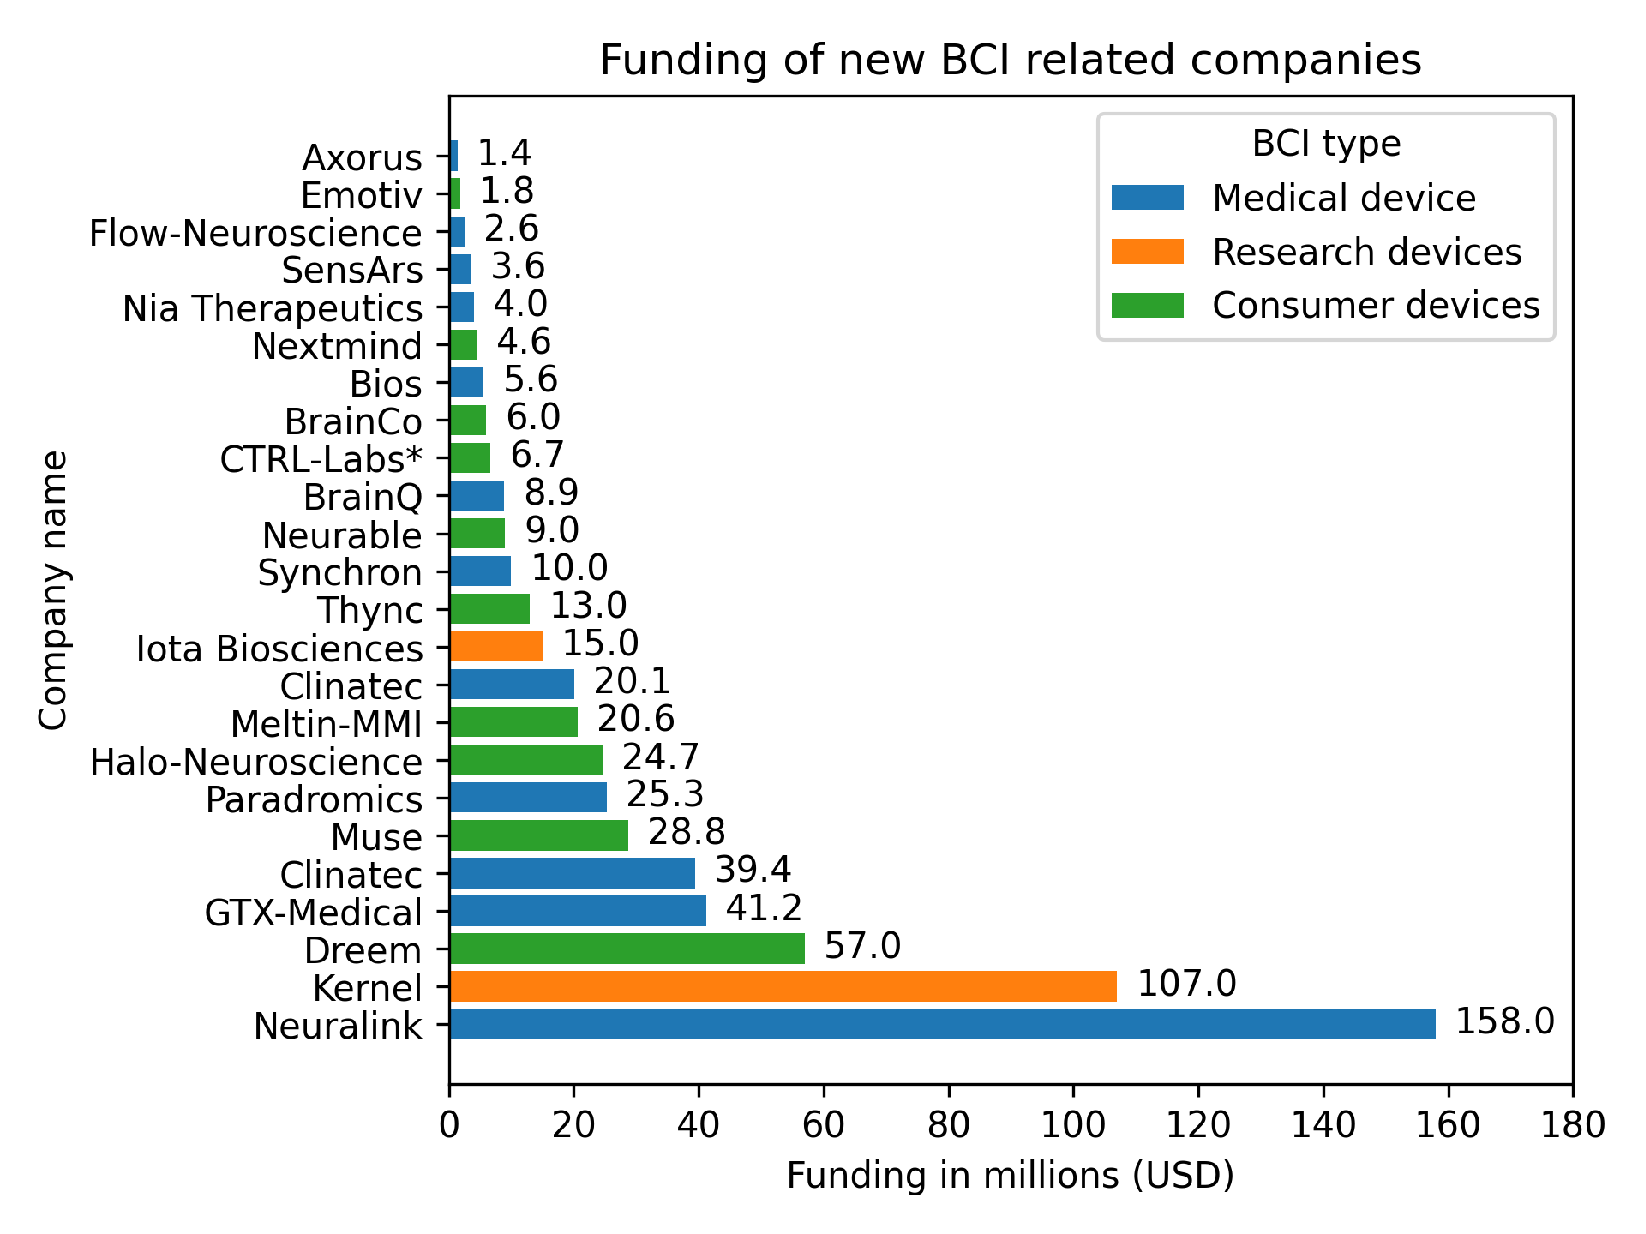
\includegraphics[width=\linewidth]{../images/introduction/funding.pdf}
    \captionsetup{width=0.9\linewidth}
    \captionsetup{justification=centering}
    \caption{Funding of newer \gls{bci} related companies depicted in millions (USD).\\Figure based on data by \citet{bci_money} from 2019. It is noted this data is limited to companies that were created after 2010 where funding information is made available.}
    \label{fig:bci_money}
\end{figure}

% - - - - - - - - - -
% improved hardware
% - - - - - - - - - -


\subsection{Improved brain-signal measuring facilities}
\label{subsec:bci_gaining_popularity_better_measuring}

\glsreset{bci}
\glsreset{hmi}
\glsreset{ux}

As \glspl{bci} are a type of \gls{hmi} relying solely on brain signals to operate, the measuring facilities for acquiring data of those brain signals have a direct impact on the capability of those systems.

Most \glspl{bci} rely on non-invasive measuring equipment that uses \gls{eeg} as a source of data and this paper will focus mainly on such measuring equipment as well.
Chapter \ref{ch:biomedical_signals} explains in greater detail what \gls{eeg} and some of its alternatives are, the equipment used for acquiring brain-signal data and more.
For this introduction, it suffices to know that non-invasive \gls{eeg} measuring equipment measures the electrical potential difference, often in \gls{mv}, between electrodes placed on the scalp.

Following Wolpaw's definition for a perfect \gls{bci} given in Section \ref{sec:bci_introduction}, the recording hardware should ideally be aesthetically acceptable and shouldn't require the assistance of a professional to install.
In recent years, new developments in this hardware have made meeting these criteria more plausible, which are adressed in this section.

% | | | | | | | | | | | | |

\subsubsection{Hardware improvements in non-invasive EEG measuring equipment}
\label{subsubsec:bci_gaining_popularity_better_measuring_hardware}

Three major hardware distinction made between the electrodes used in non-invasive \gls{eeg} measuring equipment is whether they are wet or dry electrodes, whether they are active or passive electrodes and whether communication to the processing unit happens wirelessly or not.
When considering Wolpaw's definition of a perfect \gls{bci} described in Section \ref{sec:bci_introduction}, dry-electrodes with passive amplification that connect wirelessly to the processing unit would be ideal.
However, when looking at data quality, a wired wet-electrode with active amplification is best.
Luckily, recent advancements have made these differences in data quality more acceptable, as will shortly be discussed in what follows.

Wet \gls{eeg} electrodes are electrodes which require an electrolytic gel to be applied between the electrode and the scalp.
This gel functions as a conductor and, as discussed further in Section \ref{subsec:biomedical_signals_measuring_equipment}, currently allows wet electrodes to have better data quality compared to dry electrodes \citep{wet_vs_dry, dry_electrode_status, wet_dry_comparison_experiment}.
However, wet electrodes require the assistance of a professional to correctly apply the gel which leaves behind traces after use.
Adding to this, the electrolytic gel could also cause allergic effects for the user. Due to the viscosity of the electrolytic gel changing over time, artefacts in measurements may also appear \citep{dry_electrode_status}.
These are unwanted properties and conflict with Wolpaw's vision of a perfect \gls{bci}.
The medical-grade \gls{eeg} equipment shown in Figure \ref{fig:example_eeg_measuring_devices_medical_bulky} uses wet electrodes with an electrode cap.

Advancements in dry electrodes are making the gap with wet electrodes smaller and smaller \citep{wet_vs_dry, dry_electrode_status, wet_dry_comparison_experiment}.
These dry electrodes don't require the use of an electrolytic gel and given the use of an appropriate headset can be installed on the scalp without the assistance of a professional. 
Both of these properties are in favour of Wolpaw's properties for a perfect \gls{bci}.
The main reason dry-electrodes are becoming more viable to be used in real-life environments is due to improvements in active electrode technology \citep{wet_vs_dry}.
A relatively bulky setup of these dry electrodes with active amplification is shown in Figure \ref{fig:example_eeg_measuring_devices_commercial_clean}.

Active electrodes are electrodes which do more than just forwarding their measured voltage fluctuation to the main controller board whilst passive electrodes do just that.
This is often necessary since the measured signal is of such low strength that even a short distance cable from the electrode to the main board can cause a lot of noise due to electromagnetic interference \citep{active_electrode_explained}.
To reduce this noise, a preamplifier is used which additionally amplifies the signal before transmission over the wire as opposed to only being amplified in the main controller board.
This makes the final system less compact and more expensive but is often required in anything but lab environments, especially for wireless dry electrodes, as further discussed by \citet{wet_vs_dry}.

When talking about wireless electrodes, it is not the effective electrode itself that is wireless but rather the communication between the main controller board, a board to which all electrodes are connected by wire, and the processing unit such as a computer.
Such a wireless setup is shown in Figure \ref{fig:example_eeg_measuring_devices_commercial_clean}.
Whilst a wireless approach allows for the creation of an aesthetically more pleasing system where the measuring hardware and processing hardware are physically separated, a wired connection will always remain more efficient and reliable. 
However, as discussed by \citet{bluetooth_evaluation}, Bluetooth, an open standard for wireless communication, has seen extensions that are more reliable, power efficient and capable of higher transmission speeds.
This has made wireless solutions more appealing in \gls{bci} systems but overall issues with wireless solutions, in general, will prevail.
Most important is the risk of connection loss and a higher latency resulting in a longer time between the point a signal is measured and it is received by the computational unit.

All of these advancements have enabled companies such as Muse, Dreem and OpenBCI to develop non-invasive, dry-electrode based \gls{eeg} measuring equipment with active amplification in an affordable and often aesthetically acceptable manner.
As \glspl{bci} become even more popular, a heavier focus on affordability and visuals with \gls{eeg} measuring equipment is to be expected.
These two properties were less important in previous medical settings where a patient would wear such equipment only when undergoing a test in the hospital.
Figure \ref{fig:example_eeg_measuring_devices} shows the contrast between a medical-grade \gls{eeg} recording system and one that is consumer-grade.

\begin{figure}[ht]
  \begin{minipage}{\textwidth}
    \centering
    \begin{subfigure}{.48\textwidth}
        \centering
        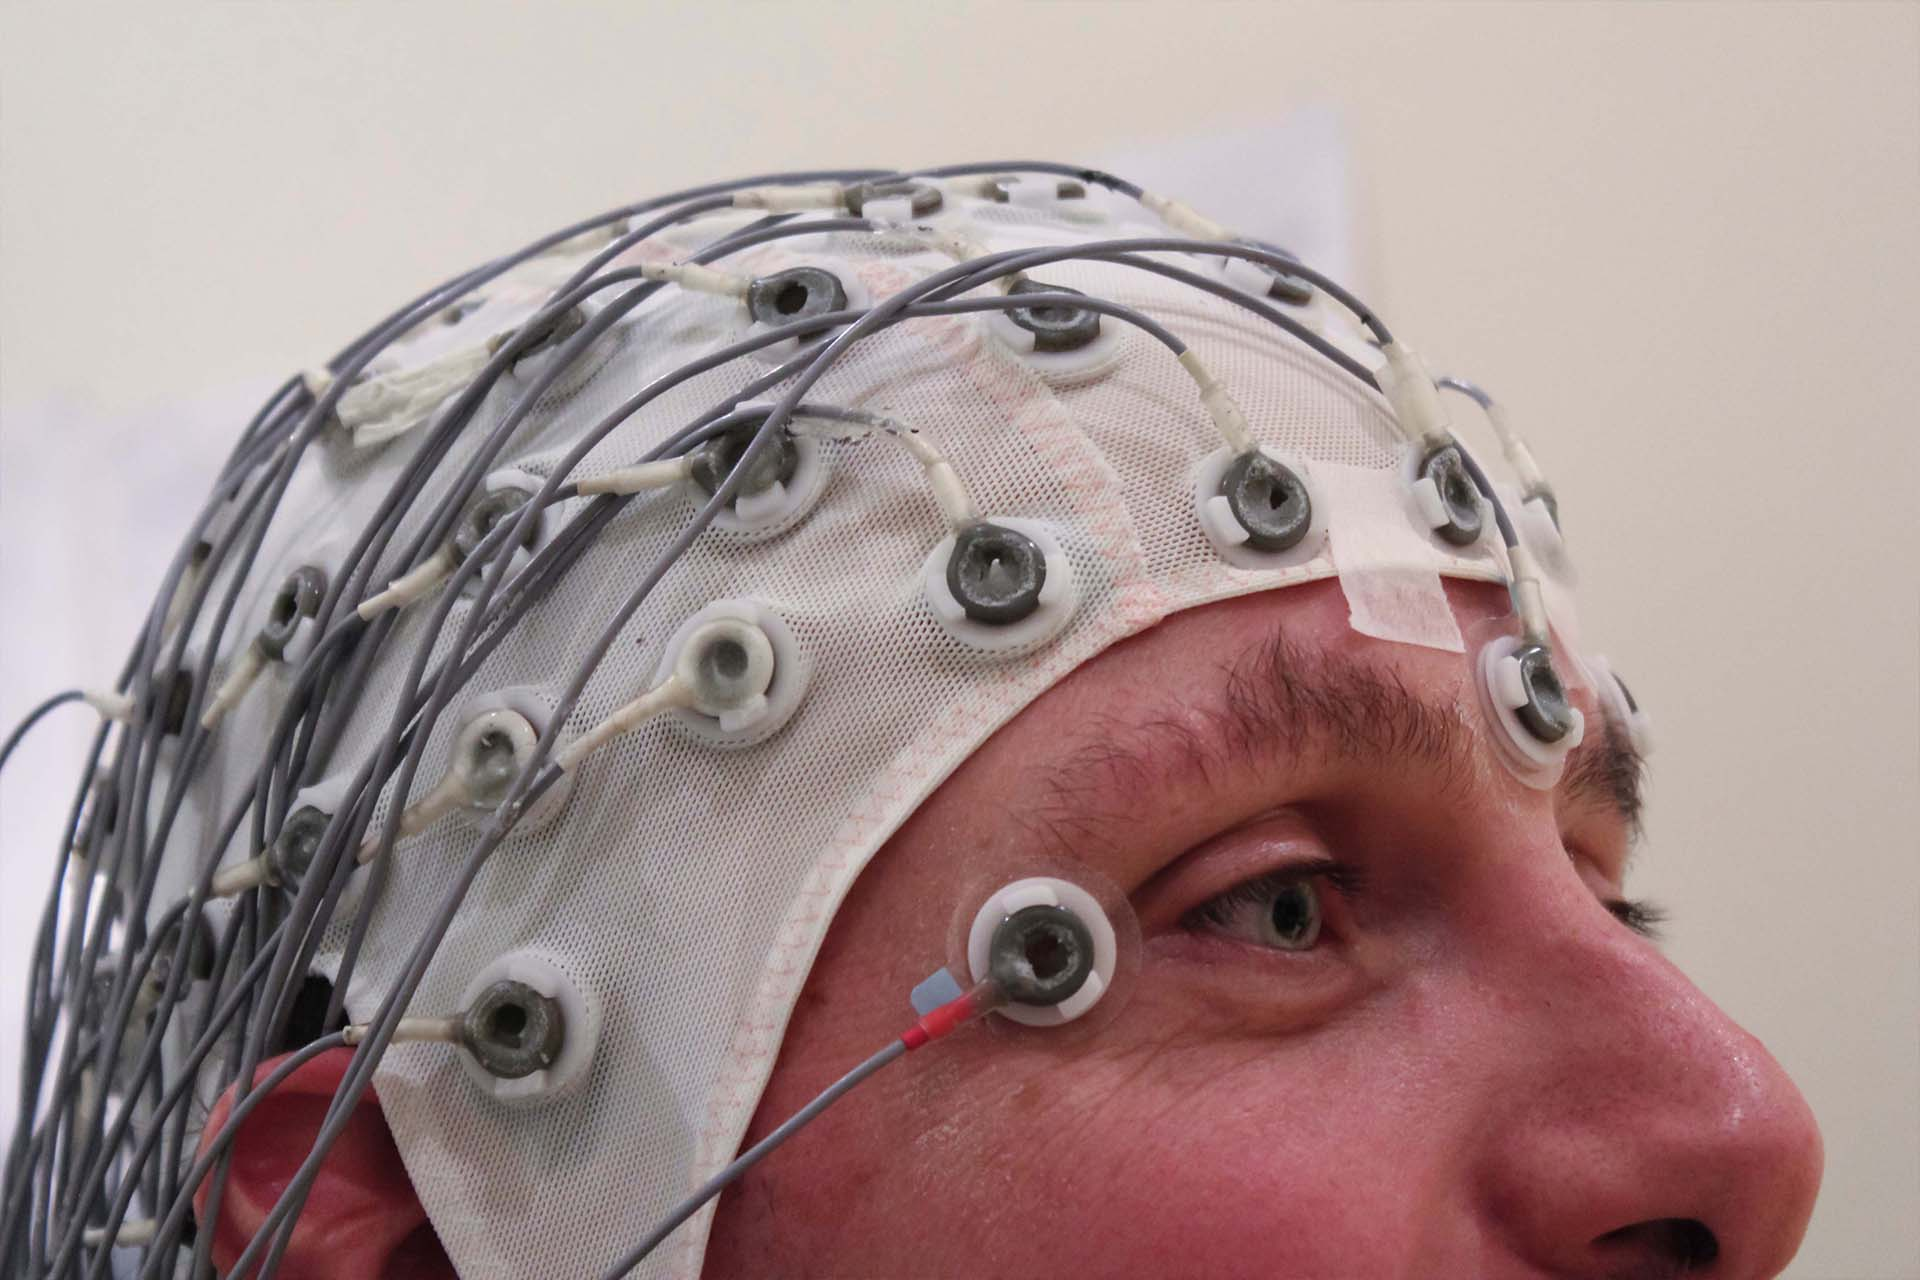
\includegraphics[width=\textwidth]{../images/introduction/wet_eeg.jpg}
        \captionsetup{width=0.9\linewidth}
        \captionsetup{justification=centering}
        \caption{Medical-grade \gls{eeg} measuring equipment that uses wet electrodes which are each connected to a separate main board via a long cable. Image from Chris Hope, CC BY 2.0, via Wikimedia Commons.\\ \hfill}
        \label{fig:example_eeg_measuring_devices_medical_bulky}
    \end{subfigure}
    \hfill
    \begin{subfigure}{.48\textwidth}
        \centering
        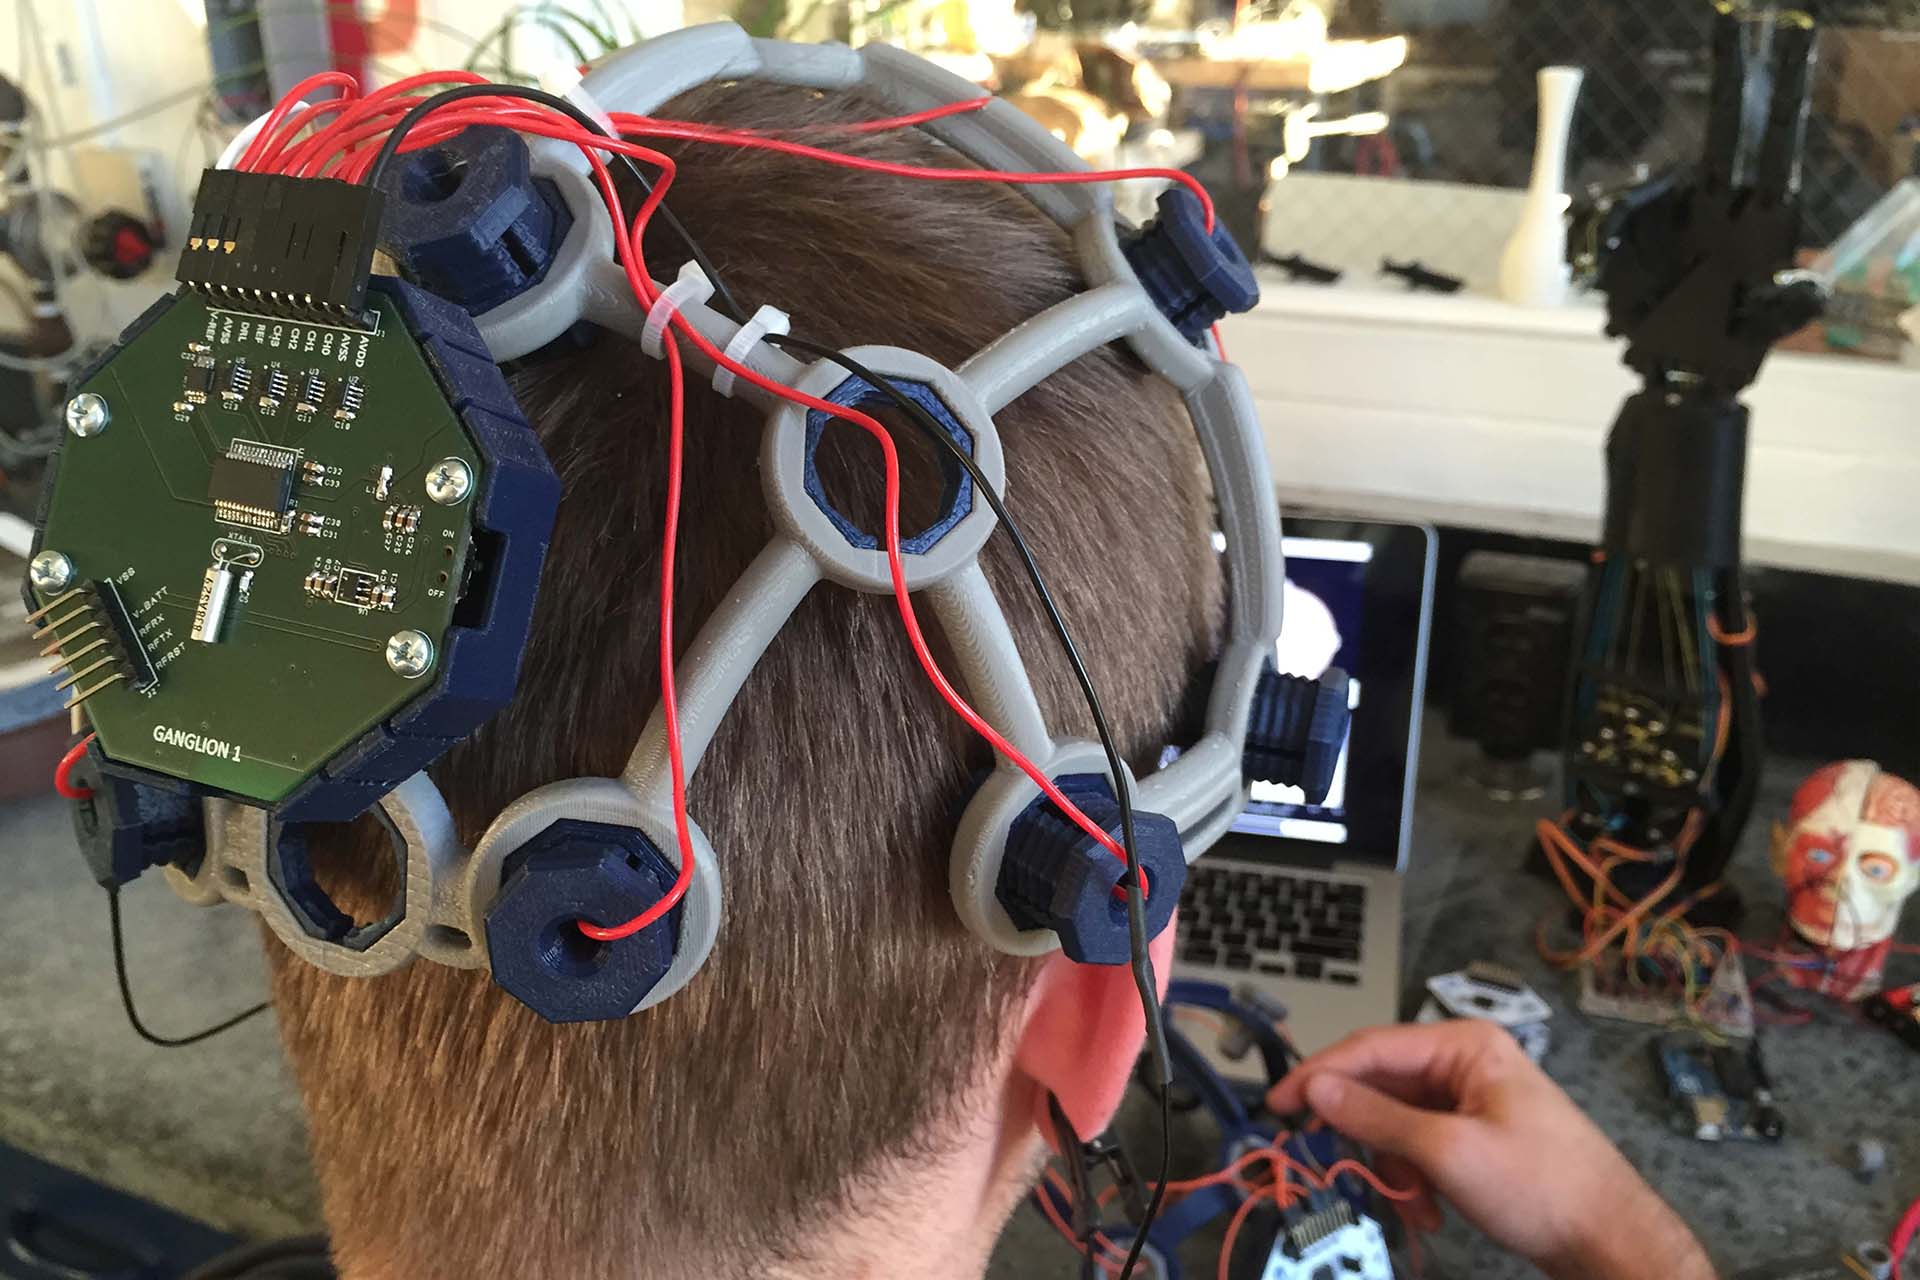
\includegraphics[width=\textwidth]{../images/introduction/openbci.jpg}
        \captionsetup{width=0.9\linewidth}
        \captionsetup{justification=centering}
        \caption{Commercial-grade \gls{eeg} measuring device that uses dry electrodes with active amplification connected to an attached wireless controller board. Image from Conorrussomanno, CC BY-SA 4.0, via Wikimedia Commons.}
        \label{fig:example_eeg_measuring_devices_commercial_clean}
    \end{subfigure}
    \captionsetup{width=0.9\linewidth}
    \captionsetup{justification=centering}
    \caption{The contrast between medical-grade \gls{eeg} measuring equipment and a consumer-grade alternative.}
    \label{fig:example_eeg_measuring_devices}
  \end{minipage}  
\end{figure}

% | | | | | | | | | | | | |

\subsubsection{Algorithmic improvements for non-invasive EEG measuring equipment}
\label{subsubsec:bci_gaining_popularity_better_measuring_software}

Whilst hardware improvements has made the collection \gls{eeg} data more affordable, reliable and accurate, one important issue still remains.
Even with the best active wet electrodes, The contrast between spatial and temporal resolution is enormous.
\Gls{eeg} is known to have a good temporal resolution but rather poor spatial resolution.
A good spatial resolution would mean that the measurement from electrodes corresponds only to a small, known region of the brain, typically underneath that electrode.
Such a correlation is helpful as it reduces noise and increases interpretability of the signal.
It also allows for fewer electrodes to be used if only the activity of certain areas of the brain is of interest.

\begin{figure}[ht]
    \centering
    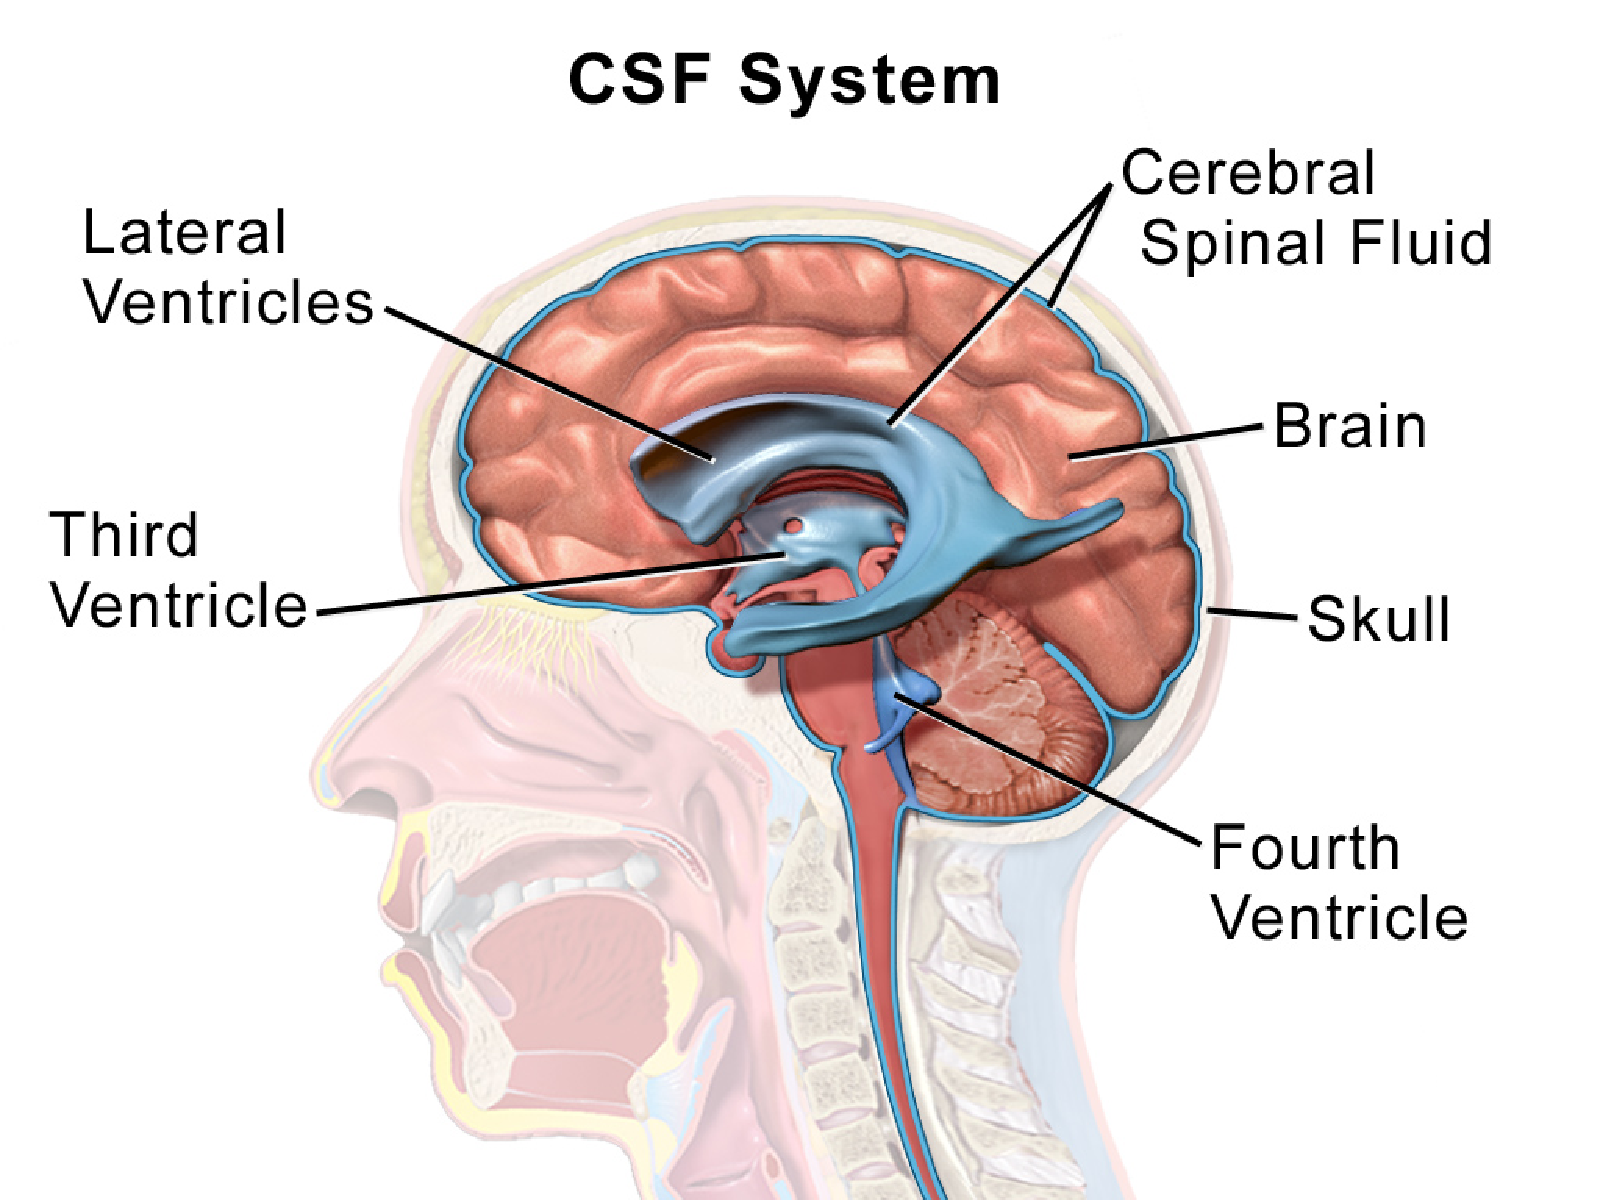
\includegraphics[width=0.7\linewidth]{../images/introduction/brain_anatomy.pdf}
    \captionsetup{width=0.7\linewidth}
    \captionsetup{justification=centering}
    \caption{The anatomy of the human head, specifically of the cerebrospinal system. Non-invasive \gls{eeg} measuring equipment is placed on the scalp, causing signals from the brain to be blocked by the skull and \glsfirst{csf} among other structures. Free to use Figure by Blausen.com staff \citep{figure_blausen}.}
    \label{fig:brain_anatomy}
\end{figure}

Thus, many attempts have been made at improving spatial resolution of \gls{eeg} but it has been proven to be a challenging task \citep{spatial_resolution}.
Besides potential noise of the measurements, this is also caused by the anatomy of the human head.
Remember that the electrodes used for non-invasive \gls{eeg} measuring are placed on the scalp, the skin of the human head.
As shown in Figure \ref{fig:brain_anatomy}, besides the scalp, different structures such as the skull and \glsfirst{csf} are in between the electrodes and the actual brain.
These components \textit{blur} and \textit{disperse} the perceived brain-signal, making it hard to track where the measured signal came from when looking at the electrical activity on the scalp.

Whilst increasing the number of electrodes placed on the skull physically limits the region under one single electrode, it doesn't guarantee an improve in spatial resolution.
Indeed, clever processing algorithms are required to correct for overlapping signals between electrodes so that the overlapped signal is correct for and the effective spatial resolution is improved.
Besides this, there is also the issue that decreasing the distance between electrodes introduces the need for placing more electrodes to cover the entire region of the brain.
This increases cost, lowers user comfort and decreases the visual acceptance of the system.
Another issue with increasing the number of electrodes and decreasing the spatial resolution means that the alignment of the electrodes on the skull is now even more prone to errors and change over time, e.g. due to movement of the user.
This makes the need for a professional higher, which is also detrimental with respect to Wolpaw's criteria for a perfect \gls{bci}.

\Citet{spatial_resolution} has found 19-electrode EEG systems to have a highly varying spatial resolution in the 20 to 40 $cm^3$ range.
Systems with 129 electrodes were found to have a spatial resolution of around 6 to 8 $cm^3$ \citep{spatial_resolution} when also using algorithmic tricks to further improve spatial resolution.
However, according to \citet{neurons_book}, around $10^7$ parallel pyramidal neurons reside in each $cm^3$ of the brain cortex.
This means the acquired data is still obtained from a incredibly large number of neurons even in the best spatial resolutions.

Whilst hardware improvements in both electrodes and headsets for better placement might improve the spatial resolution further, the spatial resolution improvements possible through hardware have been plateauing.
As was the case for the comparison between few and many electrode systems by \citet{spatial_resolution}, appropriate algorithms have to be used to effectively increase the spatial resolution.
Recently, these techniques often rely on using Laplacians \citep{improve_eeg_spatial_laplacian1, improve_eeg_spatial_laplacian2, improve_eeg_spatial_laplacian3}, although other approaches using for example \glspl{cnn} have been proposed \citep{improve_eeg_spatial_cnn}.
These techniques also have the added benefit of cleaning the time-varying signal as described by \citet{improve_eeg_spatial_comparison}.

% | | | | | | | | | | | | |

\subsubsection{Invasive BCIs try to combat the issues of EEG}
\label{subsubsec:bci_gaining_popularity_better_measuring_invasive}

The previous parts discussed how non-invasive \gls{eeg} measurements have been improved.
However, alternatives to \gls{eeg} exist for measuring brain signals, some of which are further discussed in Section \ref{subsec:biomedical_signals_measuring_modalities}.
Most notable in recent years is measuring modalities that rely on capturing brain signals by equipment directly inserted into the human body, making it an invasive approach.
One such example of an invasive measuring modality is \gls{ecog} and the most popular invasive \gls{bci} at the moment is the one proposed by \citet{neuralink_whitepaper}.
The white paper by \citet{neuralink_whitepaper} has shown that invasive \glspl{bci} could greatly exceed the data quality and visual aesthetics of even the best non-invasive alternatives.
As further discussed in \ref{subsec:biomedical_signals_measuring_why_eeg}, this invasive method places flexible electrodes directly inside the skull.
These electrodes are invisible to the human eye with the only visual component being a rechargeable wireless transmitter that is magnetically attached to the skull.
Neuralink's final aim is to make the brain-signal measuring equipment completely invisible to the human eye.

\citet{neuralink_whitepaper} has built robots to insert the electrodes inside the skull in a very precise location without the need for an open-skull operation or even anaesthesia.
This allows for a magnitude more electrodes to be installed and is expected to suffer far less from noise resulting in a far greater temporal and spatial resolution compared to \gls{eeg}.
This suggests that invasive systems are superior to non-invasive alternatives, but the fact that they are more permanent, far more expensive and invasive gives rise to technical and ethical questions.
These ethical questions are further discussed in Section \ref{sec:bci_ethical}.
From a technical standpoint, maintaining and upgrading a non-invasive \glspl{bci} is far simpler and cheaper.
The fact that you are inserting foreign objects into the brain also introduces far more health risks than non-invasive systems do.
Convincing the user to put on a headset that can be removed will also be far easier than convincing the user to get a \gls{bci} permanently implemented in their skull.

It has also been shown that the theoretical more precise temporal and spatial resolution doesn't linearly correlate with improved \gls{bci} accuracy/control, rather it seems to plateau relatively quickly with current state-of-the-art signal processing and classification techniques \citep{dropping_curve_eeg_lectrodes, more_electrodes_not_better}.
Some critics point to the dropping curve found by \citet{dropping_curve_eeg_lectrodes} to conclude that the increased electrode amount and reachable neurons achieved by \citet{neuralink_whitepaper} don't have a direct impact on the usability of \glspl{bci} in real-world applications.
Because of these aspects, the ease-of-use appeal and far cheaper price for non-invasive alternatives still outweigh the benefits offered by invasive methods for almost all but highly medical applications, at least in the opinion of the writer of this thesis.
Nevertheless, future improvements in signal processing and classification techniques could prove invasive methods to be far superior for \gls{bci} applications and the mechanical achievements so far are not to be underestimated.
An invasive system is also promising concerning Wolpaw's definition of a perfect \gls{bci} discussed in Section \ref{sec:bci_introduction}.
Once installed, it would ideally require no more assistance from a professional, is aesthetically acceptable as it can be invisible to the human eye, has signs of being far more reliable than \gls{eeg} and more.

% | | | | | | | | | | | | |

\subsubsection{Summarizing the improvement of measuring facilities}
\label{subsubsec:bci_gaining_popularity_better_measuring_summary}

Since \glspl{bci} rely solely on brain signals to operate, the measuring facilities for acquiring data of those brain signals have a direct impact on the capability of those systems.
As was discussed in this section, the most commonly used modality for non-invasive data acquisition, \gls{eeg}, has benefited from both hardware and software improvements.
From a hardware point of view, the switch to dry electrodes using active amplification and wireless connection to a computational unit has made \glspl{bci} more favourable concerning Wolpaw's criteria for a perfect \gls{bci} \citep{bluetooth_evaluation, wet_vs_dry, active_electrode_explained}.
From a software perspective, clever algorithms have enabled preprocessing of the signal to improve spatial resolution \citep{improve_eeg_spatial_laplacian1, improve_eeg_spatial_laplacian2, improve_eeg_spatial_laplacian3, improve_eeg_spatial_cnn}.
Improving the spatial resolution can also positively affect the temporal resolution due to inherent noise reduction as discussed by \citet{improve_eeg_spatial_comparison}. 
As is further discussed in Section \ref{subsec:processing_signals_general_pipeline_preprocessing}, other prepossessing techniques have also been introduced and refined further aiding in improving the data quality. 

% - - - - - - - - - -
% better hardware
% - - - - - - - - - -

\subsection{More powerful, affordable and portable equipment}
\label{subsec:bci_gaining_popularity_better_processing}

The improvements in brain signal measuring equipment have likely been influential in the gaining popularity of \glspl{bci} as it provides more precise data more affordably.
However, having the possibility of obtaining clean data is only part of the way to a perfect \gls{bci} system.
Other improvements concerning computational power, affordability and portability have also played an important role in \gls{bci} research, contributing to the rise of popularity in the process.

% | | | | | | | | | | | | |

\subsubsection{The emergence of faster and cheaper hardware}
\label{subsubsec:bci_gaining_popularity_better_processing_cheaper}

As chapter \ref{ch:processing_signals} will discuss in greater detail, working with \gls{eeg} data, or other forms of brain signal data can require computationally very heavy operations to achieve desired processing results of that data.
Luckily, together with the improvements in state-of-the-art measuring equipment, there is also an emerging supply of less accurate but far more affordable and portable \gls{eeg} measuring equipment.
Due to Moore's law \citep{moores_law} and other advancements, \glspl{cpu} and other computational hardware have also seen massive improvements in computational power.
This has made algorithms previously requiring expensive specialized computational hardware possible on the average personal computer.
All of these factors have made \gls{bci} applications, which were previously limited to lab environments with a high financial cost, accessible to a far broader public.
The availability of open-source datasets for common tasks related to brain signals has also allowed computer scientists to experiment in the field without additional hardware cost \citep{eeg_data}.

% | | | | | | | | | | | | |

\subsubsection{Splitting BCIs into multiple major components for portability and reusability}
\label{subsubsec:bci_gaining_popularity_better_processing_split_into_components}

Early attempts at making \glspl{bci} more portable and affordable include those by \citet{early_bci_drowsiness} and \citet{early_bci_multimedia}.
In essence, these applications rely on separating the data acquisition process and data processing into two standalone systems connected over Bluetooth.
Remember from Section \ref{subsec:bci_gaining_popularity_better_measuring} that Bluetooth is an open standard for wireless communication that has seen improvement in the last couple of years.
Dividing a \gls{bci} system in a data acquisition and data processing system allows for creating a lightweight measuring device to be placed on the user's head, with a heavier and bulkier computational unit to process the signals which ideally is still pocket-able.
The latter was not a trivial task and introduced the need for custom hardware at the time.
\citet{early_bci_drowsiness} used a custom-made \gls{dsp} for the task whilst \citet{early_bci_multimedia} opted for a more general \gls{fpga} based \gls{dsp}.
Whilst these were great demonstrations of how the technology could be used outside the lab, the actual usage for a bci detecting driver's drowsiness \citep[as proposed in the paper by][]{early_bci_drowsiness} and allowing multimedia control \citep[as proposed in the paper by][]{early_bci_multimedia} was rather limited.
The idea of custom-made and possibly proprietary processing hardware which focuses on a single task is also very limiting, although it does have commercial benefits.

What did stick, was the idea of splitting the hardware into two standalone parts, a wireless \gls{eeg} measuring device and a processing unit.
As discussed in Section \ref{subsec:bci_gaining_popularity_better_measuring}, a wireless connection between these two components is also favoured when taking into account Wolpaw's criteria on a perfect \gls{bci}.
It also makes it possible for smaller research teams or even individuals with a certain specialisation to take part in the highly interdisciplinary field by not requiring knowledge of all components but just the one that is of interest.
As an example, it enables computer scientists to purchase off-the-shelve affordable \gls{eeg} measuring hardware and communicate with it through provided libraries for their favourite programming language.
In most cases, the personal computer they already own is powerful enough for the experiments, especially for offline systems.
This allows for reusing existing hardware which is great from a financial perspective.
Section \ref{subsec:biomedical_signals_measuring_equipment} discusses some of the \gls{eeg} measuring equipment available on the market.
It is noted that \gls{eeg} measuring hardware is not strictly needed for a computer scientist as researchers such as \citet{eeg_data} have made excellent free-to-use \gls{eeg} datasets available.

With the introduction of the iPhone in 2007, it didn't take long for researchers to explore the idea of using a mobile phone as a processing unit for a \glspl{bci}.
\citet{early_bci_phone} were one of the first to explore this idea, with a \gls{ssvep}-based \gls{bci}.
Section \ref{subsec:biomedical_signals_brain_signals_measurable_brain_activity} will go into further detail on the types of measurable brain-signals.
In essence, such a system relies on a category of brain signals that are often easy to detect but require a specific stimulation.
This type of system can be used for a wide variety of applications.
Imagine an audio-guided tour in a museum where visitors only need to stare at a screen next to an item of interest to start hearing the explanation of that item.
This could be achieved with only a couple of dry electrodes placed on the skull in a headset that also provides the audio to the visitor.
This headset could then be connected over Bluetooth to the visitor's phone running an app for the museum tour.
The technology needed for such a system would lean close to that of so-called \textit{P300 spellers}, which have already been heavily studied \citep{p300_spellers_review, p300_keyboard_flashing, p300_spellers}.
Such a system would also fit perfectly with Wolpaw's definition of a perfect \gls{bci}, albeit oriented to a commercial setting rather than a medical one.

% | | | | | | | | | | | | |

\subsubsection{Making BCIs a one-in-all device again for profitability}
\label{subsubsec:bci_gaining_popularity_better_processing_profitibility}

Whilst the advantages of using the computational power of devices a customer already owns are clear, it also imposes some disadvantages.
For one, the varying type of computational devices is bound to give varying performance results, compatibility issues and overall limits the guarantee of a pleasing \gls{ux}.
Adding to this, the measuring equipment and processing equipment can't be connected from the factory resulting in an experience that is not plug-and-play.
From a commercial perspective, it would be easier if the system was all-inclusive and possibly patentable. 

Recent trends in computing hardware where manufacturers are shifting away from general all-purpose \glspl{cpu} and them developing their own custom \gls{cpu} architectures have shown that custom chips can outperform their general counterparts.
Patenting the architecture of those chips is possible making it commercially interesting.
Apple's mac M series processors announced in 2020 are one such recent example.
These M series processors have a neural engine that is stated to accelerate the time needed for \gls{ml} tasks\footnote{\url{https://nr.apple.com/dH8i4U3v2w}}.
\Glspl{gpu} used for autonomous driving systems also differ from general-purpose \glspl{gpu}.

Because of this, the author of this paper believes custom-made chips could create a future where the headset has a directly integrated processing unit once again.
Whilst this would make for a more attractive package for the customer and give commercial advantages to the manufacturer, it would be disadvantageous for research purposes.
The manufacturer could limit the possibilities of using the \gls{bci} for different purposes, patent promising hardware and more.
Another possible route the author of this paper sees is the use of cloud computing and fast 5G connections to also create a more simple user experience that doesn't require Bluetooth tethering to a close-by processing unit.
This approach would still leave a separation between measuring hardware and processing hardware making changes to any of the two independently easier.
Concerning Wolpaw's criteria of a perfect \gls{bci}, these approaches would also be acceptable.
This belief of switching back to all-in-one devices or using a cloud service for processing the data is further endorsed by the findings of \citet{bci_review_arnau}.
In their systematic review of \gls{bc} systems, eight of the 46 studied papers used embedded hardware and one used cloud solutions.

% | | | | | | | | | | | | |

\subsubsection{Summarizing the improvements on computational power, affordability and portability}
\label{subsubsec:bci_gaining_popularity_better_processing_summary}

To summarize, due to Moore's law \citep{moores_law} and other advancements, \glspl{cpu} among other computational hardware have seen massive improvements in computational power.
This increase in computational power has enabled more advanced processing of the data on more affordable and portable hardware.
Early attempts at making \glspl{bci} more portable and affordable focused on splitting the brain signal measuring equipment from the data processing equipment \citep{early_bci_drowsiness, early_bci_multimedia}.
The system by \citet{early_bci_phone} was one of the earliest examples of a true portable \gls{bci}-system that was affordable and relied on a smartphone as a processing unit.
It showed how working with \glspl{bci} can be done using cheap and general-purpose hardware.
The research was published at a turning point for \glspl{bci} where publication numbers on \gls{bci}-related papers started rising.
This hints that the increased affordability and portability combined with more computational power played an important factor in the rise of interest in \gls{bci}. 
The rise of \gls{bci}-related papers is illustrated in Figure \ref{fig:bci_publications} based on data by \citet{bci_progress_overview}.
\Citet{bci_review_arnau} found that papers on \gls{bc} systems using \gls{dl} have seen a steady increase over the last five years as well. 

In the future, as \glspl{bci} see more commercial applications, this separation of a \gls{bci} in a measuring component and processing component might reverse to an all-inclusive device.
This has potential downsides for scientific research but makes commercial sense.
The replacement of physical computational units in close proximity to cloud solutions is another possible evolution.

\begin{figure}[ht]
    \centering
    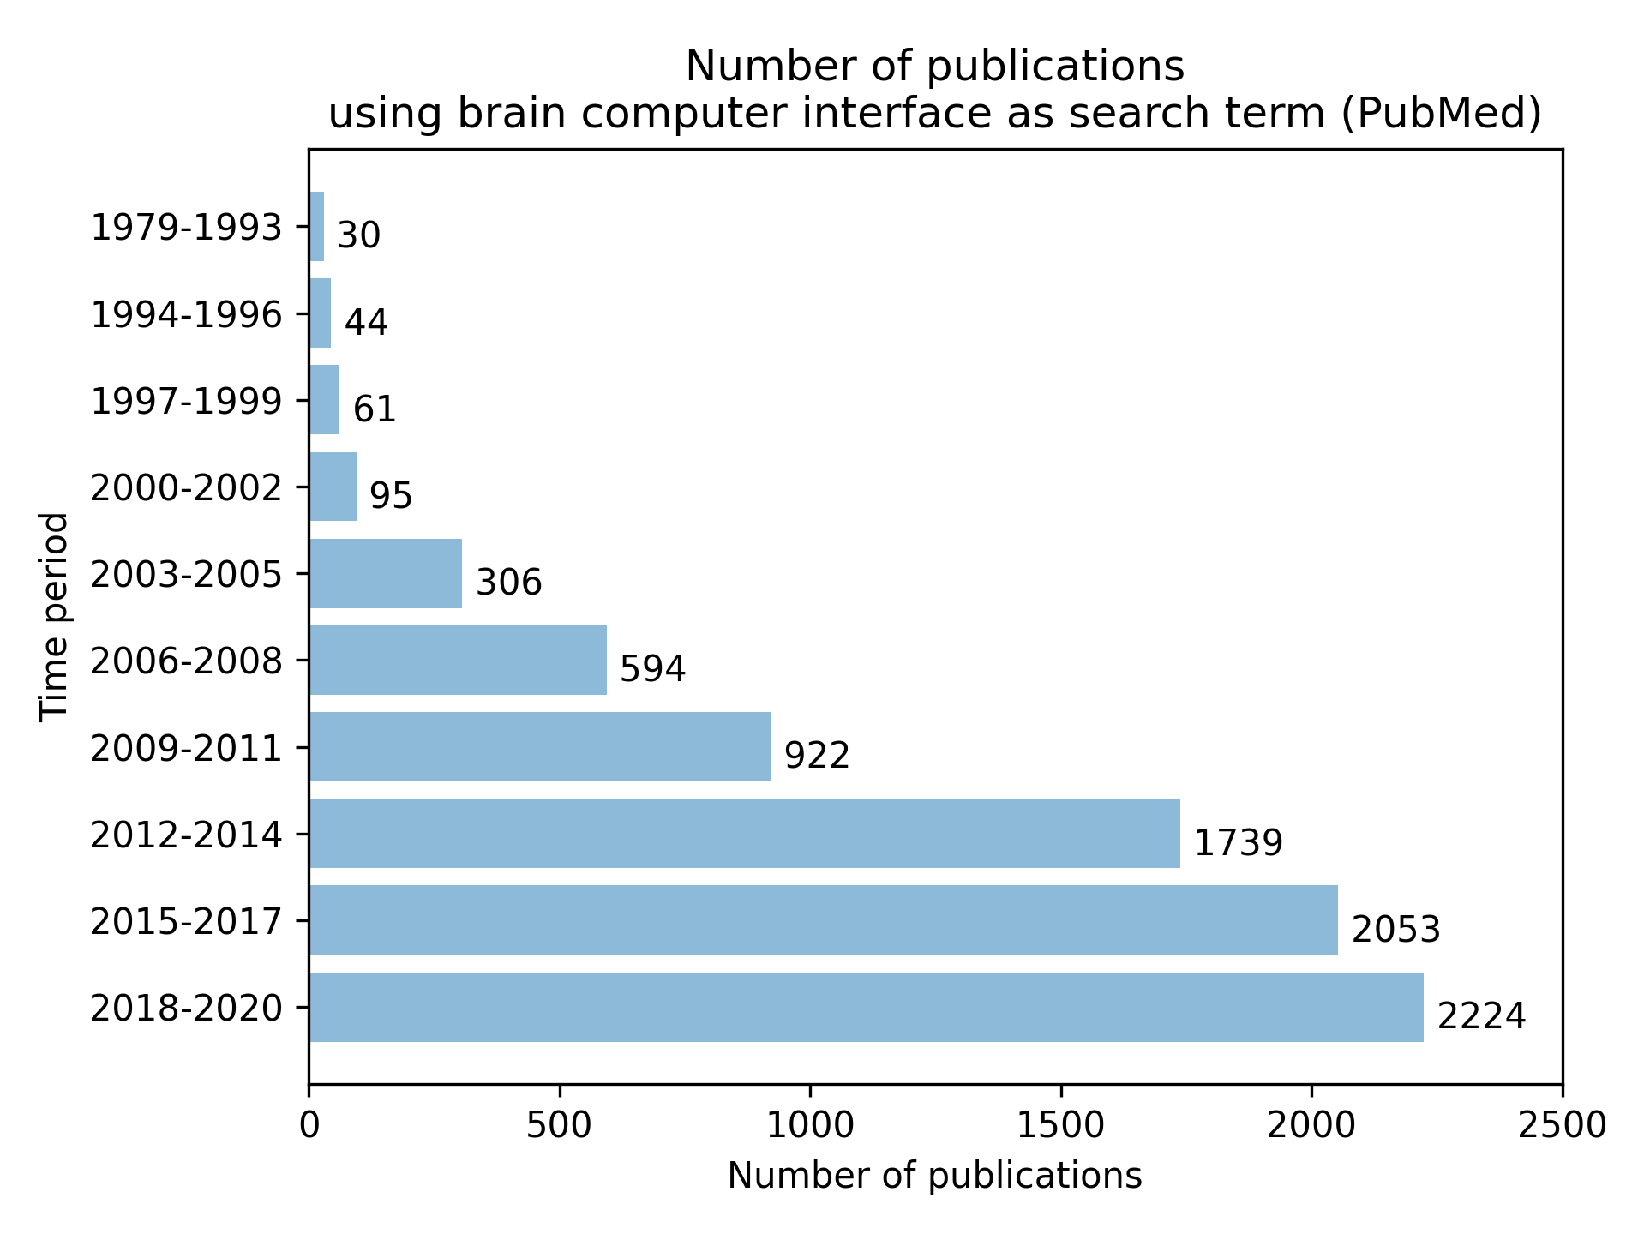
\includegraphics[width=0.8\linewidth]{../images/introduction/papers_on_bci.pdf}
    \captionsetup{width=0.7\linewidth}
    \captionsetup{justification=centering}
    \caption{Number of \gls{bci}-related papers over time. Based on data by \citet{bci_progress_overview} obtained by searching PubMed using the keyword: "brain-computer interface".}
    \label{fig:bci_publications}
\end{figure}


% - - - - - - - - - -
% better software
% - - - - - - - - - -

\subsection{Specialized data processing techniques}
\label{subsec:bci_gaining_popularity_improved_data_processing}

\glsreset{dl}

The previous sections \ref{subsec:bci_gaining_popularity_better_measuring} and \ref{subsec:bci_gaining_popularity_better_processing} discussed how both measuring and computational hardware have seen recent improvements.
Another important part of the puzzle is the algorithms that convert data from the now more user friendly measuring devices to useful actions using the now more powerful, affordable and more portable computational hardware.
Most of these algorithms are data-driven classifiers that use \gls{ml} techniques.
In more recent years, \gls{dl} techniques and alternative approaches have been incorporated in the \gls{bci} pipeline as well, which has been proven to be very successful. 
Chapter \ref{ch:processing_signals} discusses commonly used techniques in more detail and multiple \gls{ml} and \gls{dl} based \gls{bci} pipelines are discussed in later chapters of this thesis.
This section gives a more high-level summary of recent developments in the \gls{ai} field that have likely contributed to the rise in popularity of \glspl{bci}.

% | | | | | | | | | | | | |

\subsubsection{Postponing another AI winter}
\label{subsubsec:bci_gaining_popularity_improved_data_processing_no_ai_winter}

\Glsfirst{ml} and \glsfirst{dl} are techniques that fall under the \gls{ai} umbrella.
These techniques are being used as buzzwords in a whole suite of applications and it seems as if every week there is yet another big promise or threat related to \gls{ai} discussed in major news outlets.
Recent examples that have shown the world what new techniques in this field are capable of include the Go champion beating computer algorithm by \citet{alphago}, the impressive text generation model GPT-3 by \citet{GPT3} and the image generation model DALL-E by \citet{dall_e}.
This abundance of new achievements and an overall high public interest in anything that mentions buzzwords from the \gls{ai} umbrella has caused a long lasting \gls{ai} summer since the last \gls{ai} winter of the late 1980s and early 1990s.
Such an \gls{ai} summer means that there is incredible amount of funding available for improving \gls{ml} and \gls{dl} techniques among others.
This in term causes further advancements in the field of \gls{ml} and \gls{dl} which results in more impressive achievements.

However, an \gls{ai} summer also implies that an \gls{ai} winter will inherently return.
An \gls{ai} winter is a period of time where the interest in the field is reduced and thus funding and research is limited.
As discussed by \citet{new_ai_winter}, such an \gls{ai} winter may be relatively close.
This is in part due to new regulations and public backlash on the more questionable but highly profitable applications \gls{dl} is involved in.
A recent example of this is the controversy surround Clearview AI.
Here, state-of-the-art \gls{dl} image recognition algorithms are used on billions of images collected from all over the internet, including social-media platforms, to recognize almost anyone with a public profile linked to them.
As further discussed by \citet{clearview_ai}, this technology conflicts with many EU laws yet was used by multiple police departments.
Adding to this, new regulatory changes are being proposed to limit the use of algorithms which lack explainability and interpretability \citep{eu_ai_blackbox_report, explainable_ai_policy}.
This challenges many \gls{ml} and \gls{dl} approaches currently used as explained further in Section \ref{subsec:processing_signals_common_issues_exaplainable}.

Nevertheless, there is still a high amount of resources being put into \gls{ml} and \gls{dl} research.
Throughout history, these technologies have been linked with the biomedical setting a lot.
As explained by \citet{dl_and_biomedical}, \gls{dl} and biomedical data have directly influenced each other's evolution's since the 1980s.
Because of this, applications that process biomedical data have been an important factor at prolonging the current \gls{ai} summer.
Since \glspl{bci} use biomedical data as well, they have been one of the applications keeping interest in \gls{ml} and \gls{dl} research high.
This is in part due to the science-fiction properties \gls{bci} systems have creating a lot of public interest as already discussed when talking about Elon Musk's Neuralink in Section \ref{subsec:bci_gaining_popularity_big_tech}.
Thus, \gls{bci} systems, which rely heavily on \gls{ml} and \gls{dl}, are one of the research areas in these technologies that are so promising they help prolonging the current summer of \gls{ai}.

% | | | | | | | | | | | | |

\subsubsection{Improved and new ML and DL concepts have enabled more capable BCI systems}
\label{subsubsec:bci_gaining_popularity_improved_data_processing_better_ml_dl}

Most of the main concepts from both \glsfirst{ml} and \glsfirst{dl} are already multiple decades old.
As \gls{dl} is a subset of the \gls{ml} techniques, pipelines for using these techniques are very similar.
To illustrate this, a general pipeline of a \gls{cad} system used for classification is given in Figure \ref{fig:cad_pipeline} and commonly used techniques are discussed below.
It is noted that besides classification tasks, some regression problems for \gls{cad} systems exist as well.
However, such regression problems are far less common in \gls{bci} systems relying on \gls{eeg} with the systematic review article of \citet{bci_review_arnau} only finding articles on classification problems for such systems.
Because of this, this thesis focuses on classification problems.
\gls{cad} systems are used extensively in hospitals for the interpretation of biomedical images and have been studied ever since computers were invented.
The most common example of a \gls{cad} system is the classification of lung images as being either from a lung cancer patient or not, often also highlighting the nodules used for this classification.
These pipelines are very similar to the ones used for \glspl{bci}, which is further discussed in Section \ref{sec:processing_signals_general_pipeline}.

\begin{sidewaysfigure}
    \centering
    \begin{subfigure}{\textwidth}
        \centering
        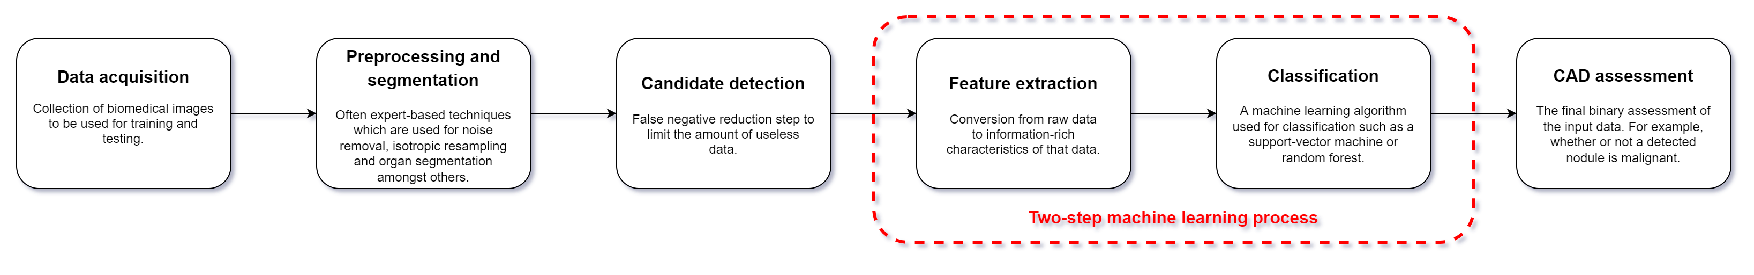
\includegraphics[width=\textwidth]{../images/introduction/cad_pipeline_ml.pdf}
        \captionsetup{width=0.9\linewidth}
        \captionsetup{justification=centering}
        \caption{General pipeline for \gls{ml} based \gls{cad} system.}
        \label{fig:cad_pipeline_ml}
    \end{subfigure}
    \hfill
    \begin{subfigure}{\textwidth}
        \centering
        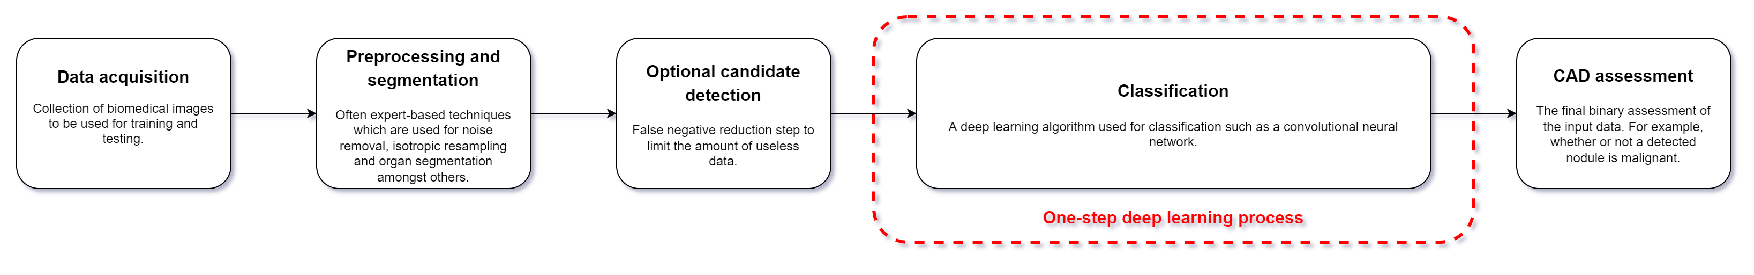
\includegraphics[width=\textwidth]{../images/introduction/cad_pipeline_dl.pdf}
        \captionsetup{width=0.9\linewidth}
        \captionsetup{justification=centering}
        \caption{General pipeline for \gls{dl} based \gls{cad} system.}
        \label{fig:cad_pipeline_dl}
    \end{subfigure}
    \captionsetup{width=0.9\linewidth}
    \captionsetup{justification=centering}
    \caption{General pipelines of a \gls{cad} system used for classification. A \gls{ml} approach is called a two-step approach as it exists from feature extraction and classification. A \gls{dl} approach is called a one-step approach as it combines both of these steps into a singular classification algorithm.}
    \label{fig:cad_pipeline}
\end{sidewaysfigure}

Traditional \gls{ml} is a commonly used name for the collection of \gls{ml} techniques that are not \gls{dl}.
Such traditional \gls{ml} rely on a \textit{two-step} process where there is both a feature extraction step and a regular classification step as is visualised in Figure \ref{fig:cad_pipeline_ml}.
Feature extraction is the process of representing the often highly dimensional and unstructured raw data using characteristic properties.
These representations are often derived from expert knowledge and are chosen by the designer of the system rather than learned from data.
With respect to a \gls{cad} system for classifying if a patient has lung cancer, these features might be the size of nodules in the lung, a metric of how round these nodules are, the \gls{hu} of certain parts of the lungs and more.
These features are then used for learning by a traditional \gls{ml} classifier.
The true challenge in these two-step traditional \gls{ml} systems lies in finding appropriate features, which can be a very time-consuming task that requires a lot of domain knowledge.
It isn't uncommon for features in \gls{cad} systems to be refined in the span of multiple years \citep{CAD_ml_dl_kbs}.
Section \ref{subsec:processing_signals_general_pipeline_features} discusses the feature engineering step in more detail and Section \ref{subsec:processing_signals_ml_and_dl_ml_classifiers} discusses traditional \gls{ml} in more detail.

Alternatively, a \textit{one-step} approach in \gls{cad} systems denotes the use of \gls{dl} in the pipeline, such as shown in Figure \ref{fig:cad_pipeline_dl}.
\gls{dl} generally differentiates itself from the previously discussed two-step traditional \gls{ml} approach by working directly on the preprocessed data rather than a feature representation of the data.
However, this isn't necessarily the case as feature extraction can still be beneficial for some \gls{dl} methods whilst others might even work better on the raw, non-preprocessed, data.
Section \ref{subsec:processing_signals_ml_and_dl_difference} discusses the difference between traditional \gls{ml} and \gls{dl} in more detail.
Intuitively, \gls{dl} models exist of multiple layers which can be seen as a graph-like structure which becomes deeper as the number of layers increases, hence the name \glsfirst{dl}.
Typically, multiple types of layers are present in a \gls{dl} approach, with the earlier layers focusing on what could be seen as gradual feature extraction steps whilst the later layers are often more tailored towards the classification of those data-driven feature outputs from the previous layers.
Section \ref{subsec:processing_signals_ml_and_dl_dl_classifiers} discusses \gls{dl} and the common variations in more detail.
A \gls{dl} approach is interesting as it can allow for skipping the feature extraction process where good features have to be found by the developer of the system.
Finding such good features can not only be time-consuming but limited expert knowledge can also make creating features that carry enough differentiating information impossible, meaning that even the best classifiers can't learn from them.
Adding to this, \gls{dl} approaches in \gls{cad} systems have also been proven to outperform state-of-the-art \gls{ml} approaches \citep{CAD_ml_dl_kbs}.
However, \gls{dl} models are more challanging in terms of explainability and interpretability as further discussed in Section \ref{subsec:processing_signals_common_issues_exaplainable}.
The challenge in \gls{dl} approaches is finding a suitable model and training it in a way such that it doesn't overfit, a phenomenon further discussed in section \ref{subsec:processing_signals_common_issues_overfitting}.
In a way, \gls{dl} allows a person with limited domain knowledge of the data to obtain a better result as it bypasses the need for manual feature extraction.
However, this is a double-edged sword as limited knowledge of the data increases the risk of bias, overfitting and other potential issues.

Relating this to \glspl{bci}, which have a very similar pipeline, and how the \gls{ml} and \gls{dl} techniques used often originate from older concepts, some of the most common \gls{bci} pipeline components are considered.
A typical traditional \gls{ml} \gls{bci} pipeline often relies on a form of the \gls{csp} technique for feature extraction.
This technique is quite old being introduced by \citet{first_csp} around 30 years ago.
Likewise, the traditional \gls{ml} classification used is often a type of \gls{svm}.
Once again, this technique was first introduced by \citet{first_svm} around 30 years ago.
Over the years, \gls{csp} has evolved and many extensions such as \gls{fbcsp} by \citet{eeg_model_fbcsp} have been introduced.
Likewise, \gls{svm} has seen many extensions and improvements \citep{svm_extension1, svm_history}.
This has resulted in the combination of these two relatively old techniques, but with recent extensions, still performing among the state-of-the-art in \gls{bci} applications using traditional \gls{ml} approaches \citep{bci_competition_review, ml_strats_used_in_papers}.
Likewise, when using a \gls{dl} approach in the \glspl{bci} pipeline, \glspl{cnn} are most commonly used \citep{ml_strats_used_in_papers, bci_review_arnau}.
This technique is again a rather old one, the foundations of which were first described by \citet{first_cnn} over 40 years ago.
Just as the \gls{csp} procedure, \glspl{cnn} have seen multiple extensions and improvements over the year, just as other \gls{dl} approaches.
Most recent and noteworthy developments are works such as that by \citet{eeg_model_hbm} which focuses on proposing \gls{cnn} architectures that can learn from very few samples and for which a described method exists to visualize the model's early layers.
Other improvements, more general to \gls{dl}, have also been made such as the development of new activation functions. \Citet{rl_activation_function_compare} discus how changing the activation function from CReLU to ReLU6 offered a 35\% performance increase while keeping other components fixed for certain experiments relying on a \gls{nn} in a \gls{rl} setting.
Thus, these improved versions of older concepts have enabled far better performance making it possible to create more capable \gls{bci} systems.

This doesn't mean that all approaches used for processing the data in \glspl{bci} rely on decades-old techniques that have improved over the years.
One interesting and relatively new approach is the use of \gls{tl} from drastically different domains.
Previously, \gls{tl} was mostly used in \glspl{bci} to train a model on data which may originate from different users performing similar but not necessarily identical tasks.
This general model is then further refined on a specific patient and task, transferring the knowledge acquired from the previous data to the new data.
When done correctly, this can provide far better performance compared to learning on the new data alone for problems where data is limited \citep{bci_review_arnau}.
As available data specific to \glspl{bci} applications remains limited, some recent research has gone into transferring knowledge from completely different domains to \gls{bci} specific data.
\Citet{tl_cnn_eeg} used a model pretrained on images and transferred it to \gls{eeg} data for a \gls{mi} task with promising results.
Other attempts at transferring knowledge from other domains, such as natural language, have also been made \citep{thesis_wolf}.


% | | | | | | | | | | | | |

\subsubsection{More open-source datasets and BCI related libraries}
\label{subsubsec:bci_gaining_popularity_improved_data_processing_open_source_data_code}

Whilst more affordable and portable measuring hardware has enabled a low-cost solution for researchers to acquire their own data, as discussed in Section \ref{subsec:bci_gaining_popularity_better_processing}, the process of acquiring \gls{bci} related data remains significantly time-consuming and can impose multiple challenges.
As addressed by \citet{bci_review_arnau} many publications don't properly report the data acquisition process, leaving a lot of ambiguity in both the meaning of data labels and how representative of the real-world the data is.
Whilst two papers might discuss a \gls{mi} task as being \textit{imagined left-hand movement}, one might have collected the data in a lab-like environment from a trained user envisioning a single squeezing shut movement of the hand whilst another might have it correspond with any envisioned movement of the fingers on an untrained and non-focused user.
On a legal aspect, as data on brain signals is biomedical data, heavy regulations are in place on how this data can be shared and used, next to the \gls{gdpr} \citep{gdpr_data_sharing, biomedical_data_privacy}.

Considering that many researchers in the field often focus on one specific component of the \gls{bci} pipeline, it is not feasible for them to go through the trouble of collecting data themselves.
Adding to this, when a researcher wants to reuse a certain component of the \gls{bci} pipeline from another author's work, the source code of their project is often not present, not well documented, or not compatible with their programming environment \citep{bci_review_arnau}.

Luckily, \gls{bci} specific data and coding libraries have been made available in recent years.
Some of the earliest \gls{bci} related datasets that are still commonly used to this day are from the \gls{bci} competitions organised by the \gls{bbci}\footnote{\url{https://www.bbci.de/competition/}}.
Of the four different competitions, two were in part organized by Jonathan R. Wolpaw, from who this thesis took the definition of a \gls{bci} and a perfect \gls{bci}, further demonstrating his importance in the field \citep{bci_competition2, bci_competition3}.
The fourth and final competition provides three \gls{eeg} datasets labelled with \gls{mi} tasks, making it a popular choice in literature.
More recent datasets include those by \citet{eeg_data}, who have put a tremendous focus on discussing all necessary details of the data acquisition process, including testing the \gls{mi} skills of each subject and providing the software and instructions given to the subjects.
Not only do these publicly available datasets allow researchers to skip the data acquisition step, but it also improves the reproducibility of their work and makes comparing it to other work using the same dataset easier.
However, there is still far from an abundance of data that can be used for training \gls{bci} pipelines compared to other fields of research.
Indeed, collecting datasets of books for \gls{nlp} learning applications or cat images for computer vision applications is a far easier task than collecting \gls{eeg} datasets for identical \gls{mi} tasks with equal data acquisitions methods.

From a code perspective, many authors still fail to deliver a copy of their source code along with their article \citep{bci_review_arnau}.
Some websites, such as Papers With Code\footnote{\url{https://paperswithcode.com/}} has been created to more easily find papers that do provide their code, but for \gls{bci} research this is still limited.
Luckily, advanced libraries have been emerging which provide a multitude of common operations from the \gls{bci} pipeline.
Perhaps the most famous of which is the Python MNE library by \citet{mne} which provides tools for organizing, visualizing and processing \gls{eeg} data such as windowing the \gls{eeg} data, performing baseline correction and determining the \gls{csp} features.
Other famous Python libraries include Braindecode by \citet{eeg_model_hbm} and EEG-DL by \citet{eeg_model_esi, eeg_dl_paper2, eeg_dl_paper3, eeg_dl_paper4} among others.
Whilst Python is the most commonly used programming language for implementing \gls{bci} pipelines and has by far the most supporting libraries, libraries for MatLab (e.g. EEGLab by \cite{eeglab_matlab}), C++ (e.g. Brainaccess by Neurotechnology\footnote{\url{https://www.neurotechnology.com/brainaccess-documentation/C++Api}}) and other popular programming languages are starting to emerge as well.
Besides these general libraries, some of the most famous articles whose source code isn't provided have also seen open-source implementation based on the original author's description.
Most noteworthy is the Army Research Laboratory (ARL) EEGModels Project which provides implementations of the EEGNet model proposed by \citet{eeg_model_eegnet} and the ShallowConvNet and DeepConvNet models proposed by \citet{eeg_model_hbm} written in Keras and Tensorflow \citep[Python DL libraries by][]{keras, tensorflow}.

% | | | | | | | | | | | | |

\subsubsection{Summarizing the emergence of specialized data processing techniques}
\label{subsubsec:bci_gaining_popularity_improved_data_processing_summary}

Besides improvements on a hardware level, both for the measuring equipment and the processing equipment, significant software improvements have also been made.
Most importantly are the improvements made to two-step traditional \gls{ml} approaches and single-step \gls{dl} approaches.
This includes improvements of the \gls{csp} feature extraction algorithm such as \gls{fbcsp} by \citet{eeg_model_fbcsp}, improvements to the \gls{svm} classifier \citep{svm_extension1, svm_history} and general \gls{dl} improvements \citep{tl_cnn_eeg, bci_review_arnau, rl_activation_function_compare}.
The introduction of more open-source datasets and libraries also aids in far faster development of new \gls{bci} pipelines and allows researchers to focus on a specific component of the \gls{bci} pipeline to improve.
The fact that \glspl{bci} still provide a science fiction feeling to the general public has also made it one of the technologies that aid in postponing another \gls{ai} winter.

Relating this to Wolpaw's definition of a perfect \gls{bci}, it becomes apparent that these software improvements play an important role in achieving the goal of a perfect \gls{bci}.
Better pipelines should allow a \gls{bci} system to function more reliably and in more challenging environments. 
Improved techniques could also improve the number of classifications a system can handle in a certain period.
This can enable the \gls{bci} system to match or even surpass the conventional interaction method it wishes to replace.
Whilst these are very important aspects of a perfect \gls{bci}, it should be remembered the user of a \gls{bci} will most likely not appreciate this evolution to the same degree a computer scientist will.
At the end of the day, an ideal processing pipeline should be one the user never notices is there, whilst a wrong classification that results in the wrong command being executed or other issues with the pipeline will result in unpleasant experiences the user will remember. 

% - - - - - - - - - -
% summary
% - - - - - - - - - -

\subsection{Summarizing the cycle of increasing popularity}
\label{subsec:bci_gaining_popularity_summary}

When looking at the number of papers published on PubMed with the keyword \textit{brain-computer interface} visualised in Figure \ref{fig:bci_publications}, a clear upwards trend is visible over the years.
This upward trend seems to have started in the 2000s and the jump was most significant around 2012.
Whilst proving which elements are responsible for this upward trend in both scientific and commercial interest isn't directly possible, this section has highlighted multiple potential reasons.
It is unlikely any one of these potential reasons is the sole reason for the increased popularity of \gls{bci} systems.
Rather, all of the discussed reasons likely influence each other as portrayed in Figure \ref{fig:cyclic_popularity_increase}.

\begin{figure}[ht]
    \centering
    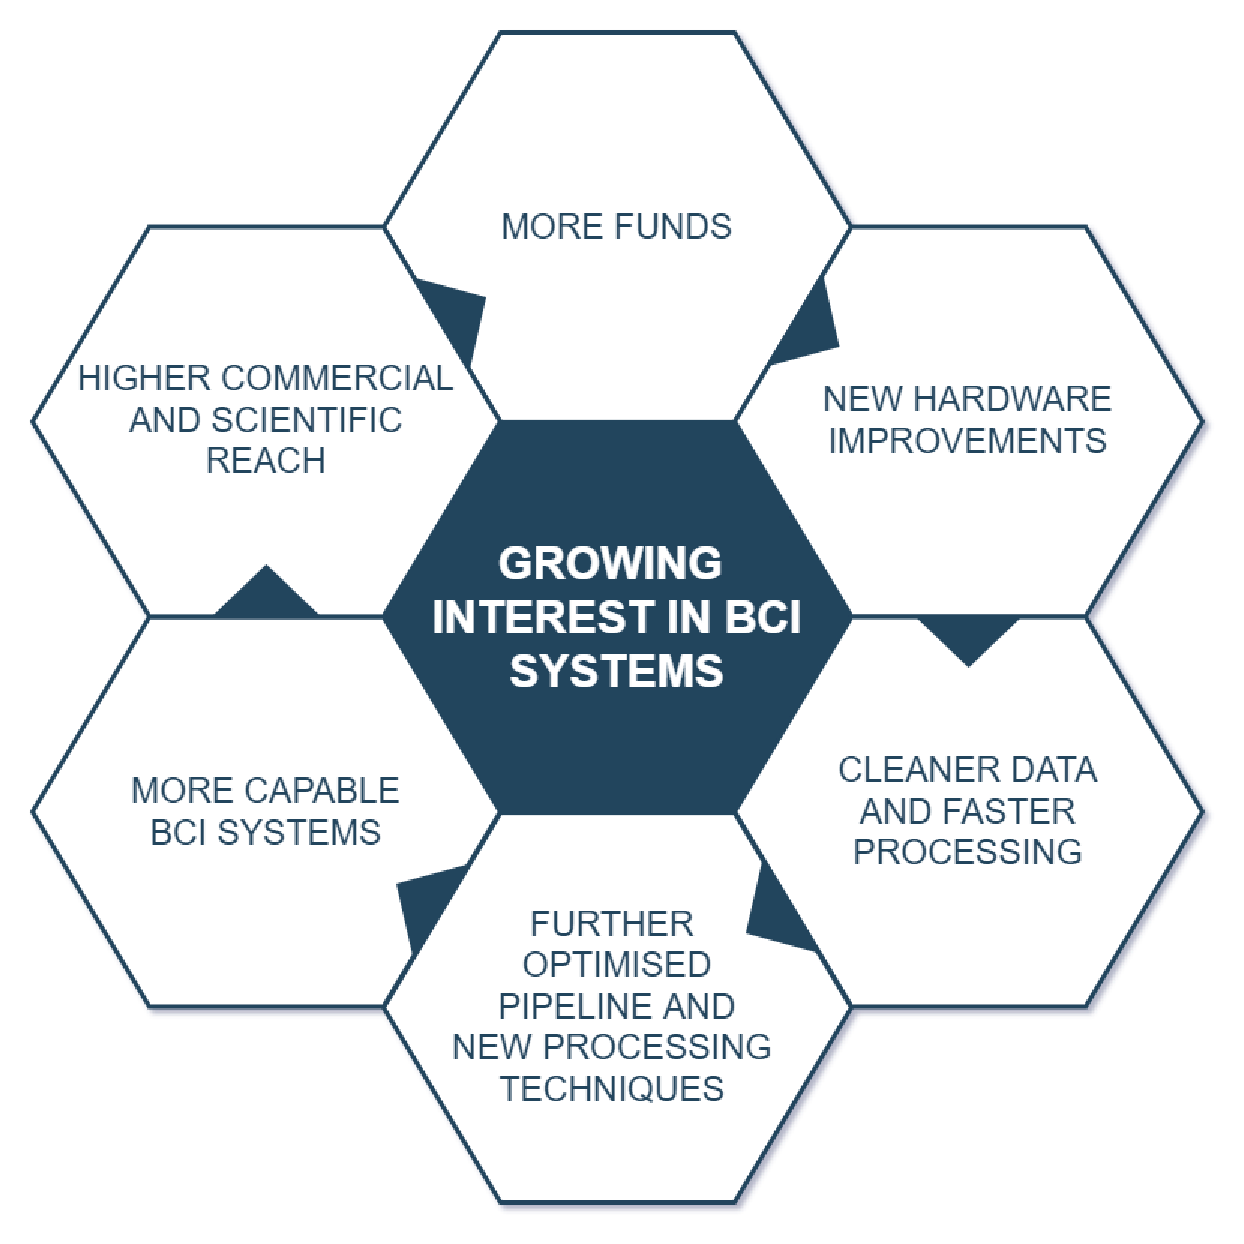
\includegraphics[width=0.7\linewidth]{../images/introduction/cyclic_interest_gain.pdf}
    \captionsetup{width=0.7\linewidth}
    \captionsetup{justification=centering}
    \caption{Summary of some of the potential reasons \gls{bci} research has seen its gain in popularity discussed in section \ref{sec:bci_gaining_popularity}. There is no clear chronological order for these events and they likely influence each other all at the same time.} 
    \label{fig:cyclic_popularity_increase}
\end{figure}

The potential reasons that were discussed can be separated into four major categories.
First, an increased interest by big-tech companies causes big funds to get into the field.
Secondly, improvements in measuring equipment allow for higher quality data and a more pleasant \glsfirst{ux}.
Third, processing equipment has seen increased affordability whilst also improving the computational power and portability allowing systems to be more affordable and capable.
Finally, more optimised software allows for better classification results and faster development of new systems.
It is highly unlikely all of these reasons have equal influence or that they are the only reasons for the improved popularity, but they should give the reader a better understanding of the context \glspl{bci} are currently in without becoming too technical.
The next section focuses on effective use cases for \glspl{bci} to let the reader understand the different capabilities of these systems even more.



% ---------------------------------------------- 
% USE CASES
% ---------------------------------------------- 

\section{Common use cases for BCIs}
\label{sec:bci_common_use_cases}

The previous section aimed to address potential reasons for the increase in popularity in \gls{bci} research.
This already discussed multiple \gls{bci} applications, showing some of the use-cases for \glspl{bci}.
When looking at Wolpaw's definition of a \gls{bci}, a \gls{bci} is nearly limitless in what it can be used for.
Whilst it should be a \textit{communication device}, this terminology can be seen rather broadly.
Most obvious is perhaps the use of a \gls{bci} as a control system, which then communicates with an external device so that it can be controlled.
Already discussed examples of this type include the multimedia control system proposed by \citet{early_bci_multimedia} from Section \ref{subsec:bci_gaining_popularity_better_processing}.
However, when using \glspl{bci} to detect common patterns of a disease, these patterns could also be communicated to a doctor and hence it could also be considered a communication device.
It should also be noted that the given definition of both a \gls{bci} and perfect \gls{bci} from section \ref{sec:bci_introduction} are around 20 and 10 years old respectively.
During the time that has passed since then, many new use cases for \glspl{bci} have emerged, especially in a commercial setting.
Thus, these definitions are by no mean the only definition for what a \gls{bci} system is and it is not uncommon to find varying opinions on what can be called a \gls{bci} system and what can't be called one.
This section aims to familiarize the reader with a broad idea of possible use cases of \glspl{bci} and to give some concrete examples whilst also addressing some of the shortcomings found in the articles describing them.
As this thesis focuses on non-invasive \gls{eeg} based \glspl{bci}, this section will also focus on non-invasive \gls{eeg} related articles.

For the interested reader, \citet{bci_review_arnau} provides more examples of \gls{bc} systems, of which \glspl{bci} are a subset, that use \gls{dl}.
The focus of \citet{bci_review_arnau} is on articles that provide at least a completely working \glsfirst{poc}, from live data acquisition to external device control.
\Citet{ml_strats_used_in_papers} reviews several \gls{bci} specific papers and focuses on the type of \gls{ml} task that is performed and which \gls{ml} and \gls{dl} techniques are used for this.
Only a few articles discussed by \citet{ml_strats_used_in_papers} have a working \gls{poc} on live data with many simply looking at the evaluation metrics of the \gls{ml} and \gls{dl} strategies.
Whilst the articles discussed by \citet{bci_review_arnau} are thus more representative of real-world performance and use-cases, finding such complete works is rather challenging.
Because this section is only meant to demonstrate potential use cases of \glspl{bci} and common shortcomings in the papers discussing them, there is no enforcement of requiring the discussed papers to have a fully working \gls{poc}.
This allows for offline systems and articles focusing on only certain components of the \gls{bci} pipeline to be discussed as well.
It also allows for discussing systems which may not strictly be \glspl{bci} but which do use almost identical pipelines, further demonstrating what is possible when working with brain signals as data.
In this regard, it is similar to the work of \citet{bci_applications} who give an overview of the most common use cases for \glspl{bci} and the challenges they are faced with.

% - - - - - - - - - -
% diseases
% - - - - - - - - - -

\subsection{Using BCIs as an automated tool in all stages of medical phenomena}
\label{subsec:bci_common_use_cases_medical_phenomena}

As \gls{eeg} is relatively affordable and portable, it is an often used modality in the hospital.
The visualisation of the measurements can be read by a specialist to diagnose a whole suite of diseases.
Especially seizure-related disorders such as epilepsy are often diagnosed through \gls{eeg} readouts \citep{eeg_epilepsy}.
Other neurological disorders such as the \gls{lis} can also be correctly identified by \gls{eeg} readouts \citep{eeg_lis_detection}.
Even the psychological field uses \gls{eeg} as a physiological measuring tool to aid in the diagnosis and psychological treatment of patients, although psychiatrists should be aware of the limitations \gls{eeg} has for them as further discussed by \citet{eeg_for_psychiatric}.
Since \gls{eeg} is used for a wide variety of diagnoses and by far the most common source of data for non-invasive \gls{bci} \citep[as discussed by][]{bci_review_arnau}, much research has gone into how \glspl{bci} can be used as an automated aid for medical diseases throughout all stages of a medical phenomena.
In general, three important distinctions are made for the stage of such phenomena and thus for the medical application of the \gls{bci}: prevention, diagnosis/monitoring and rehabilitation/restoration.

% | | | | | | | | | | | | |

\subsubsection{Using BCIs for the prevention of medical phenomena}
\label{subsubsec:bci_common_use_cases_medical_phenomena_prevention}

One popular example of prevention relates to the use of \gls{bci} systems for continuously monitoring signs of decreased attention \citep{bci_applications}.
Such a decrease in attention might show an exaggerated usage of alcohol and other drugs, which allows the user to be alerted before drinking \textit{just one more}.
Whilst it is unlikely that alcohol addicts will wear a \gls{bci} to the pub, such devices can significantly help in the reduction of traffic accidents by becoming mandatory during driving.
According to \citet{traffic_deaths}, traffic accidents were the number 1 cause of death for children and young adults.
Whilst many types of equipment are already in place to prevent traffic accidents from occurring, such as speed cameras and lane assist technology, it has been studied how \glspl{bci} can be used as a prevention measure as well.

Section \ref{subsec:bci_gaining_popularity_better_processing} discussed research by \citet{early_bci_drowsiness} as one of the first attempts to make a fully portable \gls{bci}.
As it measured drivers' drowsiness levels, the proposed system alerts or even enforces drivers to take a break from driving when drowsiness levels are too high.
Research such as that by \citet{eeg_dangerous_situation_car} has discovered that emergency situations in vehicles can be classified faster from \gls{eeg} data than the user's response, which could have a significant impact on reducing the number of traffic accidents.
\Citet{eeg_dangerous_situation_car} used a driving simulator to conduct a real-world experiment and they found that their proposed system has an accuracy of around 70\%.
One potential issue with this paper is the fact that their focus lies on this overall accuracy metric rather than providing the \textit{sensitivity} and \textit{specificity}.
Sensitivity could be seen as the accuracy of the model on positive cases (i.e. identifying a dangerous scenario as dangerous) whilst specificity denotes the accuracy on negative cases (i.e. identifying a non-dangerous scenario as non-dangerous).
However, \citet{eeg_dangerous_situation_car} do provide the \gls{roc} and provide reasoning for choosing an optimal classification threshold that resulted in this 70\% accuracy.
This threshold specifies how certain the classification prediction should be before acting on its classification.
This shows that it is important to look at more than just accuracy, as for this application being good at taking action in case a dangerous scenario is present is ideal, but taking action when there is no dangerous scenario could create a dangerous scenario itself.
Section \ref{subsec:processing_signals_general_pipeline_evaluating} discusses how to evaluate systems using different metrics and reasoning in more detail.
Many other examples of using \glspl{bci} for the detection of symptoms that can lead to traffic accidents exist. 
\Citet{eeg_motion_sickness} developed a system that could estimate motion sickness levels, which in turn could again be used to alert drivers to take a break.

The three discussed examples show how \glspl{bci} can be used in a variety of ways for the prevention of traffic accidents.
It also highlighted the importance of correct model evaluation and how a net benefit of a system is important.
For example, if the system proposed by \citet{eeg_dangerous_situation_car} would use the emergency brake each time it detects a dangerous scenario but has a poor specificity, it would heavily break in circumstances where it is not needed.
This in term creates risk if nearby drivers don't pay attention and cause a collision due to the abrupt emergency braking.
Thus, the question should be asked if a net benefit would be reached by those systems if the amount of prevented accidents outweighs the added risk of new accidents.
Likewise, it has to be considered if a \gls{bci} system is the most viable option, even if it has promising results.
Using a \gls{bci} to monitor if a driver is drunk and prohibiting him from driving if so might be more expensive and less efficient than \gls{baiid} which already exist.
Nonetheless, many applications exist for the prevention of traffic accidents and the prevention of other medical phenomena using \glspl{bci}, even if it is used as supplemental validation over existing devices and tests.
\citet{bci_applications} provides some extra examples of this type.

% | | | | | | | | | | | | |

\subsubsection{Using BCIs for the diagnosis and monitoring of medical phenomena}
\label{subsubsec:bci_common_use_cases_medical_phenomena_monitoring}

Section \ref{subsec:bci_gaining_popularity_improved_data_processing} already introduced the \glsfirst{cad} pipeline.
\gls{cad} systems, and the very similar \gls{cade} systems, using medical imagery are widely used for diagnosis and treatment monitoring in oncology and other fields.
Comparable systems exist using \gls{eeg} and other brain-signal measuring modalities for diagnosis medical phenomena and monitoring of the treatment.
The commercial Muse headset for sleep tracking that was discussed in Section \ref{subsec:bci_gaining_popularity_big_tech} is one example of a system that can be used for monitoring and diagnosing sleep patterns.

Whilst the Muse headset is a commercial product, medical \glspl{bci} exist which are made for detecting sleep patterns.
One very popular example is using \gls{eeg} for detecting sleep apnea, a medical sleep disorder.
\Citet{eeg_sleep_apnea} proposed an \gls{eeg} based \gls{bci} system for automating the detection of sleep apnea.
\Citet{eeg_sleep_apnea} named their used \gls{ml} approach \textit{Artificial Bee Colony Optimize Hermite Basis Functions}.
This paper is an example of a system that is highly specialized for a specific problem, namely detecting sleep apnea, requiring a lot of expert knowledge since it relies on a complex feature engineering step tailored towards detecting sleep apnea. 
Whilst this makes it unlikely the same pipeline can be used for the detection of other disorders, it does provide outstanding performance with a discussed sensitivity, specificity and accuracy of over 99\%.
The article by \citet{eeg_sleep_apnea} focuses on the \gls{ml} aspect of the proposed system, by re-using an existing dataset and describing only metrics related to the classification performance.
Since this system doesn't take specific control over an external device, it isn't a control system.
However, it could be argued it still communicates the detection of sleep apnea patterns and it can be deployed in a live system to alert a nurse when these patterns occur during a trial so that the nurse can pay additional attention during that period.
In this regard, naming the system proposed by \citet{eeg_sleep_apnea} a \gls{bci} is controversial, as is the case for most \gls{eeg} based systems that diagnose and monitor medical phenomena. 
Whilst \citet{eeg_sleep_apnea} don't mention the term \glsfirst{bci} in their article anywhere, in an article of a similar system, \citet{bci_sleep_apnea} do call their \gls{eeg} based detection of sleep apnea a \gls{bci}.

Many other types of diagnosis and monitoring can be done by non-invasive \gls{eeg} based \glspl{bci}.
The review article by \citet{bci_applications} addresses the detection of brain tumours \citep{eeg_brain_tumor1, eeg_brain_tumor2} and breast cancer \citep{eeg_breast_cancer}.
The review article by \citep{eeg_diagnosing_dyslexia} discusses the use of \glspl{bci} for the detection of dyslexia.
It should become apparent that many detection systems for medical phenomena can be made from non-invasive \gls{eeg} data. 
Even if these medical phenomena seem unrelated to the brain, such as for the detection of breast cancer \citep{eeg_breast_cancer}.
However, as these systems lack a true communication factor besides informing doctors or nurses, it can be argued if these systems are indeed \glspl{bci} w.r.t. Wolpaw's definition of a \gls{bci} given in Section \ref{sec:bci_introduction}.

% | | | | | | | | | | | | |

\subsubsection{Using BCIs for the rehabilitation and restoration after medical phenomena}
\label{subsubsec:bci_common_use_cases_medical_phenomena_restoration}

Restoration of lost mobility and rehabilitation is the third and final stage of most medical phenomena.
In this stage, a \gls{bci} can be of aid to both the medical staff and patient.
Out of the three discussed stages it is also the one that has seen the most \gls{bci} related research.
One reason for this is that many techniques for the restoration of lost mobility and rehabilitation rely on \gls{emg}, a modality used for measuring muscle-based \glspl{biosignal}.
Famous examples of such \gls{emg} based systems include prostheses which are connected to the remaining muscles of an amputated body part or an exoskeleton which is placed over body parts to strengthen their movement or re-enable them. 
Whilst in general \gls{emg} based systems far outperform \gls{eeg} based systems for prosthesis and exoskeletons, the \gls{emg} modality does not apply to patients suffering from an impaired neuromuscular system.
Thus, for these patients an \gls{eeg} based solution may offer them a possibility of regaining mobility again.
Since \gls{eeg} based \glspl{bci} for prosthesis and exoskeleton control are very common research in the \gls{bci} field, it will be discussed further in it's own section, Section \ref{subsec:bci_common_use_cases_prosthesis_exoskeleton}.

\Glspl{bci} have found their usage in other aspects of the rehabilitation and mobility restoration process as well.
In neurological rehabilitation, \glspl{bci} can function as a tool for guiding both patients and medical staff in what abnormalities are present in the brain and how they can be circumvented.
Intuitively, these \gls{bci} systems aim to improve the brain's ability to adapt itself based on experience.
This self-adapting property of the brain is known as brain plasticity or neuroplasticity.
A well-developed \gls{bci} system could show patients and medical staff which regions of the brain are currently being used and which types of brain signals and abnormalities are being detected.
This information could then be relayed to the patient through various means so that it induces neuroplasticity.
Such systems are still in development and require sophisticated neurological expertise that falls outside the scope of this master' thesis.
However, they are very promising and the interested reader is referred to the overview provided by \citet{bci_rehabilitation}.
It is noted once more this paper was co-authored by Professor Jonathan R. Wolpaw, which has been discussed in this paper multiple time for his definition of a \gls{bci} and a perfect \gls{bci}.

Another area that is often researched in the rehabilitation and restoration process, is using \glsfirst{mi} tasks to improve recovery of control over certain body parts.
The main idea behind such systems is to let the patient perform a \gls{mi} task, which doesn't require effective movement of the body part with reduced control.
This \gls{mi} task can then be classified by the \gls{bci} system based on the \gls{eeg} data and an exoskeleton is used to perform that motion as passive feedback.
Most commonly, a pedalling \gls{mi} task is used to control a motorized pedal, which evokes \gls{erd} patterns resulting in a greater potential for lower-limb recovery.
The works by \citet{pedal_mi_rehabilitation1} and \citet{pedal_mi_rehabilitation2} discuss such systems in greater detail.
Likewise, stroke rehabilitation and a reduction of the effects from the Parkinson's disease can be achieved with \gls{bci} guidance as well, as further discussed by \citet{parkinson_stroke_reduction}.

It is noted that many more \gls{bci} applications exist for preventing, monitoring and controlling diseases than those discussed here.
The work by \citet{bci_in_medicine} highlights some use-cases of \gls{bci} in medicine for example.

% - - - - - - - - - -
% prosthesis exoskeleton
% - - - - - - - - - -

\subsection{Using BCIs for prosthesis and exoskeleton control}
\label{subsec:bci_common_use_cases_prosthesis_exoskeleton}

Arguments were given why the medical applications of \gls{eeg} processing systems discussed in Section \ref{subsec:bci_common_use_cases_medical_phenomena} can or can't be considered \gls{bci} systems.
The main discussion revolves around the kind of communication that the system does.
To some authors, a system that alerts or visually informs medical staff based on processed data from \gls{eeg} can be considered a \gls{bci} system whilst others specifically expect an external device to perform a specific action based on the brain signals to name a system a \gls{bci} system.
The latter would be a type of control system, as the \gls{bci} controls an external device.
In a review article by \citet{bci_review_arnau}, it is found that among \gls{eeg} based \gls{bci} control systems using \gls{dl}, the control of robotic arms is most popular in research.
This section will discuss the use of \glspl{bci} as a control system for prostheses and exoskeletons.

% | | | | | | | | | | | | |

\subsubsection{Why BCIs are used for prosthesis and exoskeleton control}
\label{subsubsec:bci_common_use_cases_prosthesis_exoskeleton_why}

Most of the current robotic prostheses and exoskeletons rely on muscular activity in the body.
Just like brain activity can be measured by non-invasive \glsfirst{eeg}, muscular activity can be measured by non-invasive \glsfirst{emg}.
For example, patients who have had a partial loss of a body part often still have muscular activity in the remaining body part.
In the case of surgical amputation, the amputation is often done such that as much muscle remains to ensure as much possible muscular activity also remains.
These patients can then often still generate the muscular activity that would have been required for moving the missing body part.
This muscular activity can then easily be measured with the \gls{emg} modality, which is in general of higher signal quality than \gls{eeg} \citep{hybrid_eeg_emg_prosthesis}.
This \gls{emg} data can then be processed to classify the wanted movements and control robotic prostheses.
\Citet{emg_prosthetics} discuss the design and development of such a system based on \gls{emg} in greater detail.
Since the overall pipeline of such \gls{emg} based systems is quite comparable to the pipeline of \gls{eeg} based \glspl{bci}, many of the processing techniques are similar to those discussed in this thesis.
Alternatively, when the body part is still fully intact but the control over that part is lost or requires extra support, an exoskeleton may be used similarly.
Just like robotic prostheses, most exoskeletons rely on \gls{emg}.
A thesis by the German \citet{emg_exoskeleton} highlights the fundamentals of \gls{emg} based exoskeletons.

As was already touched upon in the rehabilitation and restoration part of Section \ref{subsec:bci_common_use_cases_medical_phenomena}, \gls{emg} measurements are not applicable for all patients.
In particular, people who have neurological diseases, limiting the production of the required muscular-based \glspl{biosignal}, fall outside the scope for these solutions.
However, the viability of robotic prostheses and exoskeletons for these patients has been steadily on the rise as \gls{eeg} based \glspl{bci} have been proposed for this purpose.
\Citet{bci_prostheses} give an in-depth systematic review of upper and lower limb exoskeletons and robotic prostheses controlled by \gls{eeg}-based \gls{bci}.
Just as was the case for rehabilitation and restoration discussed in Section \ref{subsec:bci_common_use_cases_medical_phenomena}, these systems often make use of brain signals measurable after imagined movement.
This process of thinking of movement but not doing the movement is known as \glsfirst{mi} and further discussed in Section \ref{subsec:biomedical_signals_brain_signals_measurable_brain_activity}.


% | | | | | | | | | | | | |

\subsubsection{The risk of using BCIs for prosthesis and exoskeleton control}
\label{subsubsec:bci_common_use_cases_prosthesis_exoskeleton_risk}

Whilst it is clear to see why \gls{eeg} based \glspl{bci} are promising for prosthesis and exoskeleton control from the discussion above, it should be noted that there is also a great risk in doing so.
\Citet{bci_prostheses} address the high risk associated with failed instructions for robotic prostheses and exoskeletons.
This means that the risks that can follow from misinterpreted instructions of exoskeletons and robotic prostheses are of such a degree that even high accuracy systems might not be good enough to guarantee a net benefit for the user.
This could be the reason that the review article by \citet{bci_review_arnau} didn't find any \glsfirst{poc} applications for exoskeleton or prosthesis control using \gls{eeg} based \glspl{bci}.
However, \citet{bci_review_arnau} did find many papers controlling an external robotic arm which is not connected to the body and thus not seen as a prosthesis.

\Citet{bci_prostheses} also highlight that whilst multi-label classification of \gls{eeg} is possible with considerable accuracy in an offline lab setting, the number of detectable classes is limited in a real-time and real-life environment.
Because of this, \gls{eeg}-based systems in these applications still have some challenges to overcome to match the precision and reliability of \gls{emg} counterparts.
Whilst improvements regarding these aspects have been made since the work of \citet{bci_prostheses} was published, the main challenges remain to this day, especially when using affordable systems.
Because of this, widespread adoption of \gls{eeg}-based exoskeletons and robotic prostheses is still very limited.


% | | | | | | | | | | | | |

\subsubsection{Promising steps towards BCI controlled prosthesis and exoskeleton control}
\label{subsubsec:bci_common_use_cases_prosthesis_exoskeleton_promosing_steps}

Whilst the discussed risk has caused widespread adoption of \gls{eeg}-based exoskeletons and robotic prostheses to still be very limited, promising steps are being made to bring them to market.
These systems mainly focus on robotic arms, which are not strictly a prosthesis but they pave the road to \gls{bci} controlled arm prosthesis in the future.
These proposed systems often rely on incorporating supplementary information such that risky movements are cancelled, even if the \gls{bci} requests them. 
\Citet{bci_mi_robotic_arm_collision_avoidance} proposed such a system to control a robotic arm not only through a \gls{eeg} based \gls{bci} working with \gls{mi} tasks but also by using obstacle avoidance algorithms to reduce the risk of harmful contact, computer vision for object detection to get a better idea on the possibly wanted interaction and eye-tracking to gather extra information surrounding the user's intention.
Other successful research on making more reliable \gls{bci} systems for controlling robotic arms is done by \citet{eeg_robot_arm1, eeg_robot_arm2, eeg_robot_arm3, eeg_robot_arm4}, these articles are also included in the review article on \gls{dl} based \gls{bc} systems by \citet{bci_review_arnau}.

Whilst limb prostheses, currently being pilot run through robotic arm research, are one of the most common and researched types of prostheses, they are only a fraction of all prostheses in existence.
Everything from dentures to artificial breasts can also be labelled as a type of prostheses.
For example, visual prostheses such as bionic eyes are another type of prostheses that has active research in the \gls{bci} field.
Not only can \gls{bci} systems improve visual prostheses, many of the existing visual prostheses could be seen as a special type of \gls{bci} system as a whole.
Both the works by \citet{bci_blind_assist_review} and \citet{bci_vision_assist_review} give an overview on the progress in visual prostheses in the \gls{bci} field.
These \glspl{bci} are often invasive and opposed to only reading brain activity, they can also stimulate the brain and other parts of the body.
Through this stimulation or by other means, the user can regain some form of vision from these \gls{bci} systems.
Second Sight is one of few companies that has commercially made visual prostheses with approval from the \gls{fda}.
Their system is discussed in the overview on \gls{bci}-related vision restoration systems by \citet{bci_vision_assist_review}.
The international trial by \citet{second_sight_trial} on the products of Second Sight shows promising results, although it is noted the study is performed by Second Sight employees and not by an independent research team.
The exact working of visual prostheses or, more specifically, Second Sight products is not of interest for this work, but the recent decisions of Second Sight company reveal one of the largest risks of invasive \glspl{bci} and \glspl{bci} in general.
Due to the discontinuation of some of the Second Sight products, hundreds of users are left without product support for a system that shaped their everyday life.
Besides this, the now non-functioning product is still present inside their body.
The issues and ethical questions this brings to the table are discussed further in Section \ref{subsec:bci_ethical_e_waste}.


In summary, hybrid systems like the one by \citet{bci_mi_robotic_arm_collision_avoidance} are very promising as they can greatly reduce the risk involved in many \gls{bci} systems, such as prostheses-related applications, whilst also increasing the overall accuracy of the system.
Section \ref{subsec:bci_common_use_cases_improving_existing_system} discusses more of these hybrid systems but where \glspl{bci} are used as supplementary component to an existing system.


% - - - - - - - - - -
% improving system
% - - - - - - - - - -

\subsection{Using BCIs to improve the working of existing systems}
\label{subsec:bci_common_use_cases_improving_existing_system}

The previous sections discussed the use of \glspl{bci} as a control system for prostheses and exoskeletons.
Whilst this approach was promising for certain patients, the high risk associated with such systems meant that developing reliable systems relying solely on \gls{eeg} based \glspl{bci} was not yet possible \citep{bci_prostheses}.
One area that did see success was the use of \textit{hybrid \glspl{bci}} as a control system for robotic arms.
Such hybrid systems combines \gls{bci} techniques with other techniques to create an overall system that is more accurate, safe and reliable and thus complies more with Wolpaw's definition of a perfect \gls{bci}.

The discussed hybrid systems from Section \ref{subsec:bci_common_use_cases_prosthesis_exoskeleton} considered the \gls{bci} as the main component with the other techniques, such as computer vision, added as support and improvement to it.
There are also multiple examples of where a \gls{bci} system is added as an \textit{extra component} to an existing system and thus not considered the main component.
This allows for \glspl{bci} to find use cases in non-trivial domains.
To demonstrate this, an extension to classical hearing aids using an \gls{eeg} based non-invasive \gls{bci} is discussed in this section.
This section also addresses the use of \glspl{bci} to make \textit{smart homes} more accessible for people with a handicap and the elderly.
It also addresses some other examples of hybrid \glspl{bci}.


% | | | | | | | | | | | | |

\subsubsection{Extending hearing aid systems with BCIs}
\label{subsubsec:bci_common_use_cases_improving_existing_system_hearing_aids}

According to \citet{hearing_aids_noise_reduction} over 450 million people suffer from disabling hearing loss.
Most solutions to hearing loss rely on a microphone to capture environment audio which is then amplified and played through a speaker that is placed in or near the ear.
Most commonly, the microphones used for amplification are integrated inside the speakers that are placed in the ear to form a stereo setup that mimics regular hearing.
This is not always ideal when there is a lot of ambient noise.
Sometimes using an external directional microphone placed closer to the audio source of interest can form a solution.
For example, placing a microphone on the desk of a professor teaching in a noisy room of students.
However, this solution is not applicable in all situations.
Thus, most hearing aids include some noise suppression on the microphones directly to filter out ambient noise and amplify noise coming from human speech.
\Citet{hearing_aids_noise_reduction_mandarin} evaluated such noise suppression for Mandarin-speaking users and found the results to be good but not ideal, as there is a lot of variation in human speech tone making it hard to detect what is and what isn't ambient noise.

Even when such a noise suppressing filter would work optimally, people with hearing aids often still have trouble understanding people when multiple speakers are close-by at once.
Recent research by \citet{bci_hearing_aid_direction} has shown that using a non-invasive \gls{eeg} based \gls{bci} can improve traditional hearing aids in solving this problem.
\Citet{bci_hearing_aid_direction} does this by determining which speaker a user is listening to by analysing directional queues from the measured brain-signals.
If this information would be communicated to the hearing aids, it can allow them to optimize the microphones to pick up speech from that area only, filtering out other speakers.
Whilst great in theory, \citet{bci_hearing_aid_direction} discuss how a long waiting time to determine the area of interest challenges the practical usability of their system as of now.
Nonetheless, it shows one of many non-trivial ways a \gls{bci} could be used as an extension of existing systems to improve them.



% | | | | | | | | | | | | |

\subsubsection{Using BCIs to improve accessibility of existing applications}
\label{subsubsec:bci_common_use_cases_improving_existing_system_improve_accessibility}

There are still a lot of applications which lack support for people with disabilities or people with less technical skills.
Take for example the growing ecosystem of smart home applications, since it aims to automate many tasks such people might find difficult or impossible to perform, it can be very beneficial to these people.
However, conventional interaction methods are app-like through touch screens mounted all around the house.
Such interaction methods are not fit for people with limited movement capabilities or technical knowledge.

Since \gls{eeg} based \glspl{bci} are known to work well for conscious people that can learn how to effectively do \glsfirst{mi} tasks, it is often seen as a solution to provide novel interaction method with existing applications to improve accessibility.
\Citet{bci_smart_home_app} were one of the first to explore the idea of using a \gls{bci} for smart home control as they believed it could greatly improve the quality of life for the elderly and people with a handicap.
They used the Emotiv EPOC headset as a non-invasive source for the \gls{eeg} using dry electrodes and achieved high accuracy results through a primitive binary selection interface.
This means that it seems to comply with most properties of Wolpaw's definition for a perfect \gls{bci} except for one of the most important ones, it is not at all as fast as the regular interaction method.
Adding to this, their system doesn't make use of actual brain signals but rather relies on muscular activity, such as smirks and eyebrow movement.
This movement of the facial muscles is known to provide an easily detectable artefact in the \gls{eeg} and is often used as a supplementary input for the \gls{bci} system.
As section \ref{subsec:biomedical_signals_measuring_artefacts} will discuss in greater detail, such an approach has many negatives.
Finally, the system of \citet{bci_smart_home_app} was tested on four subjects but the article fails to deliver exact details on this experiment and it is assumed the participants were neither elderly nor people with a handicap.

Whilst this means the system by \citet{bci_smart_home_app} isn't a true \glsfirst{bci} due to the use of \gls{eeg} artefacts and the paper has questionable scientific value, it was one of the first to explore the idea of using a \gls{bci} for smart home control.
Since then, more articles have studied this idea using effective brain signals.
\Citet{feasibility_bci_smart_home} discuss this in their feasibility study about using \glspl{bci} for smart home control.
The article by \citet{feasibility_bci_smart_home} does include clear details on the experiment setup which includes two people with a handicap among 12 other healthy subjects.
It was found that the people with a handicap had an 81\% average accuracy whilst the healthy subjects only had a 77\% average accuracy.
Due to the low sample size, this difference in results is likely not statistically significant but these accuracy numbers are usable when taking into account the small risk of failed actions in basic smart home control systems.

% | | | | | | | | | | | | |

\subsubsection{Other examples of hybrid BCIs}
\label{subsubsec:bci_common_use_cases_improving_existing_system_smart_home}

Section \ref{subsec:bci_common_use_cases_prosthesis_exoskeleton} already discussed the use of a hybrid \gls{bci} system where computer vision, eye tracking and other technologies were used in combination with a \gls{bci} system to create a more reliable and accurate final system for robotic arm control \citep[as proposed by][]{bci_mi_robotic_arm_collision_avoidance}.
With existing algorithms such as the real-time grasp detection algorithm, GraspNet, by \citet{graspnet} for low-powered devices, it is very easy to envision how they can be used to improve a \gls{bci} related system.
Articles which propose a fully working \gls{poc}, such as the ones reviewed by \citet{bci_review_arnau}, often require these additional algorithms to ensure safe working in real-world environments.

One very interesting hybrid solution is the use of a non-invasive \gls{eeg} based \gls{bci} system with measurements from non-invasive \gls{emg}.
\Citet{hybrid_eeg_emg_prosthesis} proposed such a hybrid \gls{eeg}-\gls{emg} system for upper limb prosthesis control.
Since \gls{emg} is known to be a more accurate modality for prosthesis control, the system by \citet{hybrid_eeg_emg_prosthesis} uses \gls{emg} for movement of the prosthesis where possible and supplements it with \gls{eeg} data for determining the other wanted movements.
In particular, the proposed prosthesis by \citet{hybrid_eeg_emg_prosthesis} uses \gls{emg} present in the remaining upper arm muscles for elbow motion and \gls{eeg} for determining the desired wrist, grip and finger
motions.
The \gls{emg} part, which also imposes the greatest risk, had an accuracy of over 90\% whilst the \gls{eeg} part has an accuracy of over 65\%.

The combination of \gls{eeg} and \gls{emg} can also be used for other purposes.
\citet{thesis_arnau} proposed the use of both \gls{emg} and \gls{eeg} data for training a classifier which then relies solely on \gls{eeg} input for making final classification predictions.
Since the number of combinations to create hybrid \gls{bci} systems are nearly endless, it is left to the reader's imagination to come up with other potential use cases.

% - - - - - - - - - -
% P300 vs eye tracking
% - - - - - - - - - -

\subsection{Using BCIs as an alternative for eye tracking}
\label{subsec:bci_common_use_cases_bcis_replace_eye_tracking}

\gls{bci} systems relying on P300 signals where already briefly mentioned in Section \ref{subsec:bci_gaining_popularity_better_processing}.
As further discussed in section \ref{subsec:biomedical_signals_brain_signals_measurable_brain_activity}, a P300 signal is a positive bio-electrical wave measurable with \gls{eeg} around 300ms after a specific stimulus occurred.
This specific stimulus consists of a rare and contrasting stimulus when the user was focusing on what is otherwise a relatively static object with a frequent stimulus \citep{eye_tracking_vs_p300_comparable}.
The most famous example is the use of a computer screen showing elements in a grid-like pattern as the static object with a frequent stimulus and flashing one specific element as the rare and contrasting stimulus.
If the element the user was focused on flashes, the P300 signal will be present and relatively easily detectable in non-invasive \gls{eeg} measures.
A clever design of the interface can enable a wide variety of \gls{bci} applications.
This section will highlight a few of these applications.
It is noted that other types of stimulus can be used, such as auditory ones, to evoke a P300 signal.
However, this section focuses on the discussed, visual, grid-based methodology.

With such visual P300 based \gls{bci} relying on the before-mentioned method of focusing on a part of the screen and using flashing patterns to recognise which part the user is focused on, a viable alternative would be eye-tracking technology.
This makes the effective use of these types of \gls{bci} systems debatable, an issue that is also further discussed in this section.

% | | | | | | | | | | | | |

\subsubsection{Why a low learning curve makes P300-based BCI systems attractive}
\label{subsubsec:bci_common_use_cases_bcis_replace_eye_tracking_why_p300}

In general, \glspl{bci} using the P300 signal are often used as they have a low learning curve and there is a relatively low variation in performance between users compared to other types of \glspl{bci} \citep{p300_spellers, p300_spellers_review}.
The reason these systems have a low learning curve is due to their simple user interface and a combination of a system that generalises well and that has been studied thoroughly for the use of \glsfirst{tl}.
Early examples of using \gls{tl} for P300 related \glspl{bci} include those by \citet{p300_speller_tl}.
Adding to this, P300 signals can be detected with non-invasive \gls{eeg} using dry electrodes, which are available in multiple \gls{eeg} measuring headsets at affordable prices in a comfortable and visually pleasing package, as further discussed in Section \ref{subsec:biomedical_signals_measuring_equipment}.
Whilst these factors hint that such \gls{bci} systems comply with Wolpaw's definition for a perfect \gls{bci} addressed in Section \ref{sec:bci_introduction}, it will become clear in this section that the communication rate of these systems is still a limiting factor.

However, these aspects do make it possible for P300-based \glspl{bci} to be rapidly configured and used by a new user.
All of this aids in creating a pleasant \glsfirst{ux} even if the communication rate is low, as shown by user studies such as the one by \citet{p300_speller_real_life2}.
Other types of \gls{bci} systems, such as those relying on \Glsfirst{mi}, can have a tedious training procedure in advance.
This can cause psychological burden and other side effects for the user.
This gives rise to multiple ethical challenges, some of which are discussed in Section \ref{sec:bci_ethical}.
Considering these things, P300 based \glspl{bci} are an interesting choice as a \textit{first \gls{bci}} to introduce the user to the possibilities of \gls{bci} systems.
This might make it easier for the user to move to a more capable and sophisticated system that has a steeper learning curve, higher cost and more demanding training.

Research on the \gls{ux} is often overlooked by initial \gls{bci} system proposals, where the focus is often on objective numerical measures such as speed, accuracy, sensitivity and specificity.
However, as discussed by \citet{thesis_arnau}, user studies are essential to even consider using a proposed \gls{bci} system in the real world.

% | | | | | | | | | | | | |

\subsubsection{Using BCIs for P300 spellers}
\label{subsubsec:bci_common_use_cases_bcis_replace_eye_tracking_p300_spellers}

By far the most common usage of the P300 signal is to create \textit{p300 spellers}, an idea first described by \citet{first_p300_speller}.
In its simplest form, P300 spellers simply show the alphabet as grid elements and let the user spell words letter-by-letter.
More complex forms can use auto-correction to correct faulty classifications, reducing the effective error of the system.
Advanced text prediction can also be used to show complete words or sentences for selection, increasing the communication rate as opposed to letter-by-letter input.
Other techniques can also further increase the reliability and communication rate of the system.

As such, P300 spellers are examples of novel interaction methods that aim to replace keyboards for those who don't have the required capabilities to operate them.
Especially patients with severely limited motor skills and communication capabilities such as people suffering from serious cases of \gls{als} or \glsfirst{lis} can benefit from these systems by regaining basic communication skills \citep{p300_spellers, p300_spellers_review}.
Whilst wrong classifications in a speller application could result in unpleasant situations, it is clear that the risk involved is far smaller than with \gls{bci} system used for controlling prostheses and exoskeletons such as discussed in Section \ref{subsec:bci_common_use_cases_prosthesis_exoskeleton}.
This makes P300 spellers one of the few types of \gls{bci} systems that are actively being used in the real world.

\Citet{p300_speller_real_life} performed a usability study of P300 spellers with 20 \gls{als} patients in a real-life environment.
According to \citet{p300_speller_real_life}, most participants achieved over 70\% accuracy, which is in line with the findings of \citet{p300_spellers_review} and \citet{p300_speller_real_life2} in similar studies amongst other types of patients.
More interestingly, even though the accuracy wasn't extremely high, all participants of the experiment by \citet{p300_speller_real_life} succeeded in the given tasks.
This is in part due to our ability as a human to understand typo's in words and sentences relatively easily.
Another important factor is that the studied system makes use of the earlier discussed auto-correction and text-prediction techniques.
Whilst far from advanced variants of these techniques were used, it almost doubled the communication rate of the P300 speller already with the mean number of correct symbols per minute going from 3.6 to just over 5.

Whilst 5 symbols per minute is significantly slower compared to traditional communication skills, it enables useful communication for those who can't communicate through regular means.
It should also be considered that these results are for people suffering from \gls{als}.
These people can have difficulties with controlled eye movement or rapid eye movement which results in a slower operation speed compared to able-bodied persons.
However, since it is so slow compared to the regular interaction method of able-bodied persons, it is far from a perfect \gls{bci} when taking into account Wolpaw's definition of a perfect \gls{bci}.
A similar study by \citet{p300_speller_real_life2} focuses more on the \gls{ux} for \gls{dmd} patients using P300 spellers.
This study has shown that P300 spellers can be used by \gls{dmd} patients with satisfactory results in a pleasant manner for the user, even if the communication rate is slow.

% | | | | | | | | | | | | |

\subsubsection{Using the P300 signal for other BCI applications}
\label{subsubsec:bci_common_use_cases_bcis_replace_eye_tracking_p300_other_applications}

When taking a broader look at P300-based \gls{bci} systems using a visual grid system, they are just a mechanism for recognising which portion of the screen a user is looking at.
These grids are often of a limited size, such as 6 by 6, for the best trade-off between accuracy and communication rate.
The effective content of the grid and the actions taken upon classification can vary widely.
This has enabled the exact technology of P300 spellers to be easily adapted for other applications.

One such example is the \textit{Facebrain} application by \citet{facebrain}.
Facebrain provides a non-invasive \gls{eeg} based \gls{bci} for interacting with the social media platform Facebook.
In essence, it's a regular P300 speller with the first screen(s) representing possible actions to take on the platform.
When text input is required, a regular P300 speller user interface is presented.
This allows a user to operate almost all of Facebook's functionalities with only a P300-based \gls{bci}.
The application by \citet{facebrain} is one of many that shows the same strategy and classification algorithms as P300 spellers can be used for a wide variety of applications by changing the meaning and functionalities of the shown grid elements.
Rather than showing symbols, a complete image could be shown and separated into grid elements as well.
\Citet{p300_drone} used this idea by showing a live video stream from a quad-copter and moving it towards where the user is looking based on the P300 signal after flashing different portions of the image.
However, as the video live stream is not static, the contrast between the flash and regular screen content shrinks making the P300 signal less noticeable and thus the classification task harder.

% | | | | | | | | | | | | |

\subsubsection{Why eye tracking may still be preferred}
\label{subsubsec:bci_common_use_cases_bcis_replace_eye_tracking_eye_tracking_better}

Whilst the discussed P300 applications have shown success in achieving their goals, the effective real-world use of such systems can still be debated.
The communication rate is slow and for able-bodied users, traditional eye-tracking can far outperform these systems \citep{eye_tracking_vs_p300_comparable}.
Adding to this, as P300 signals are a type of \gls{erp}, there are some known limitations and issues with techniques relying on them as well.
The \gls{bci} handbook by \citet[Chapter~26]{bci_handbook} discusses the crowding effect, adjacency problem, repetition blindness and user discomfort amongst other issues \glspl{erp} have.
Most of these problems arise from the often limited space for sending visual stimuli without overlap and the changing behaviour of both the brain and participant's experience after a prolonged session where many stimuli have been applied.

Multiple articles have been written on when and why a P300-based \gls{bci} might be preferred over a regular eye-tracking system \citep{eye_tracking_vs_p300_comparable, p300_eyetracking_slower}.
The experiments performed by \citet{eye_tracking_vs_p300_comparable} compared the accuracy and communication rate of visual P300 based \glspl{bci} against traditional eye-tracking solutions.
\Citet{eye_tracking_vs_p300_comparable} found the accuracy of both systems to be comparable but the communication rate of eye tracking solutions was around 50\% faster.
However, when questioning the ten participants of the study, it was found that there is a higher preference for the \gls{bci} system than the eye-tracker.
Whilst favourable for the \gls{bci} alternative, the results of the study by \citet{eye_tracking_vs_p300_comparable} should be interpreted with caution.
The participants of their study were all able-bodied persons and the eye-tracking experiments were always performed last.
This and other aspects of their methodology are bound to introduce bias in the results.

A study by \citet{no_interest_in_using_p300} compared the use of eye-tracking software and auditory P300 based \glspl{bci} for a patient suffering form the \glsfirst{lis}.
Whilst the patient was able to work with both systems autonomously, there was a strong preference for the traditional communication strategy which relied on a human to determine the wanted communication of the patient.
This preference was purely based on the \gls{ux} rather than the communication rate.
Whilst only being an experiment based on a singular participant, it does show how automated systems for regaining basic communication might cause a negative psychological impact on the user.
Thus, the results found by \citet{eye_tracking_vs_p300_comparable} on \gls{ux} are in direct contrast with the results from the experiment by \citet{no_interest_in_using_p300}.
However, \citet{no_interest_in_using_p300} lacked a study of visual P300 based \glspl{bci}, so it could be that such a system would be preferred. 

Similar conflicting results are present on other aspects of visual P300 based \glspl{bci} as well.
One debate that has been active for years is the dependence of P300-based \glspl{bci} on the capability of a user to look directly to a single target for a prolonged time.
As discussed by \citet{p300_eye_gaze}, it has been argued that this dependence is low as peripheral vision allows the user to focus on the desired element even if the eyes aren't directly rotated towards the element.
This would be favourable for P300 solutions compared to eye-tracking solutions as some users might not have the required muscle control to point their eyes to a specific point for prolonged periods, a task known as eye gazing.
However, the study by \citet{p300_eye_gaze} does show a dependence of P300-based systems on eye gaze and they argue the effective uses of visual P300 systems should be reconsidered.
Yet, the review article by \citet{bci_eye_gaze} addresses multiple articles which concluded through real-world tests that being capable of eye gazing is not necessary for effective use of P300-based \glspl{bci}.

These contradicting results on the use of P300-based \gls{bci} applications make it hard to determine which kind of system would be usable in the real world, providing a net benefit for the user.
It also shows that promising objective results such as a high accuracy and communication rate are not guaranteed to provide a system which is enjoyed by the end user.
Thus, many proposed systems require follow-up articles focusing on performing in-depth real-world experiments with the target population to conclude if they are worthwhile.
However, doing such a study in the same article proposing the new novel system would mean that one singular article takes an incredible amount of time.
This is contradictory to the expectations of many researchers in the field to publish a certain amount of articles yearly.
However, the latter is an ethical dilemma that entails a higher risk of \textit{sloppy science}.

% - - - - - - - - - -
% other use cases and summary
% - - - - - - - - - -

\subsection{Summary on the use cases for BCIs}
\label{subsec:bci_common_use_summary}


Since \glspl{bci} can be seen as a novel interaction method for controlling external devices, the possible use-cases are endless.
Even for the discussed P300 based \gls{bci} systems alone, a huge variety of applications can be created as addressed in Section \ref{subsec:bci_common_use_cases_bcis_replace_eye_tracking}.
This has caused review articles to focus solely on these types of \gls{bci} systems or even subset of those types of systems \citep{p300_review_article1, p300_review_article2, p300_review_article3}.

Thus, addressing all possible use cases for \glspl{bci} is far outside the scope of this thesis.
For this section, the goal was for the reader to obtain a more general insight into the most studied uses for \glspl{bci}.
In this regard, it succeeded in addressing all of the most popular use cases of \glspl{bci} as \gls{bc} systems in the real world as found by \citet{bci_review_arnau} and the most interesting use cases of \glspl{bci} addressed in the review article by \citet{bci_applications}.
It also highlighted that current real-world applications still rely on other technologies to limit risk and improve accuracy as standalone non-invasive \gls{eeg} based \glspl{bci} are still not accurate and reliable enough for most real-world usage.
Some of the main positive and negative points of the discussed articles were also addressed.

Most notable from this section is the fact that objective measures are only a small part of making a system that can be used in the real world.
Take for example the discussed experiment by \citet{p300_speller_real_life} which studied the use of P300 spellers by patients suffering from \gls{als}.
With a classification accuracy of 70\% and only 5 symbols per minute, the objective measures from this system look terrible compared to able-bodied alternatives such as regular keyboard typing.
However, \citet{p300_speller_real_life} found the users to have enjoyed the use of the P300 spellers and when taking into account the options available to the target users rather than able-bodied users, the objective measures are far more impressive.

However, even the articles which perform experiments that take into account the \glsfirst{ux} can sometimes cause conflicting results.
Take for example the discussed differences between the found user experience of P300 based \glspl{bci} between the experiment by \citet{eye_tracking_vs_p300_comparable} and \citet{no_interest_in_using_p300}.
Able-bodied persons from the experiment by \citet{eye_tracking_vs_p300_comparable} mentioned a pleasant \gls{ux}.
A more representative real-world study by \citet{no_interest_in_using_p300}, who looked at a singular patient suffering from \gls{lis} showed that this person had no interest in using such systems as a replacement for the existing human-based communication system which was already present.
Even-though speed and autonomous use were far better and the \gls{ux} according to the able-bodied persons was great, the \gls{ux} for this person suffering from \gls{lis} was not good enough.
Thus, the \gls{ux} is something that can only truly be measured when performing the experiments for an extended period with the target audience of the system, not through a single experiment on able-bodied participants.
It is hard for an able-bodied person to understand that the confrontational aspect of \glspl{bci} on the limitation a user has can outweigh the benefits it seemingly offers.
This and other more ethical questions are also addressed in Section \ref{sec:bci_ethical}.

To summarize, as a \gls{bci} performs actions based on brain signals, a very fitting analogy could be made: \textit{a \gls{bci} could do anything you can think of}.
That is, of course, only true in theory.
Due to limited knowledge of the brain \citep{brainmapping} and limitations in what can be measured, a \gls{bci} can only truly do what you can think of in a \textit{measurable way}.
Still, this is a whole lot of applications and an overview diagram of the most important ones is given in Figure \ref{fig:bci_use_cases_diagram}.
This diagram is not only based on the use cases discussed in this thesis but also those discussed in the articles by \citet{bci_review_arnau} and \citet{bci_applications} among others \citep{bci_review_book_chapter, bci_review, bci_in_medicine, bci_history, bci_review_monkey, bci_handbook}.
From Figure \ref{fig:bci_use_cases_diagram}, it should become apparent that most short-term goals of \glspl{bci} still lie in improving the quality of life for people with disabilities.
However, the rise in popularity of \glspl{bci} in the gaming industry and amongst other big tech companies, as discussed in Section \ref{subsec:bci_gaining_popularity_big_tech}, shows there is a potential future where \glspl{bci} find more real-life use-cases in other fields as well.

\begin{figure}[ht]
    \centering
    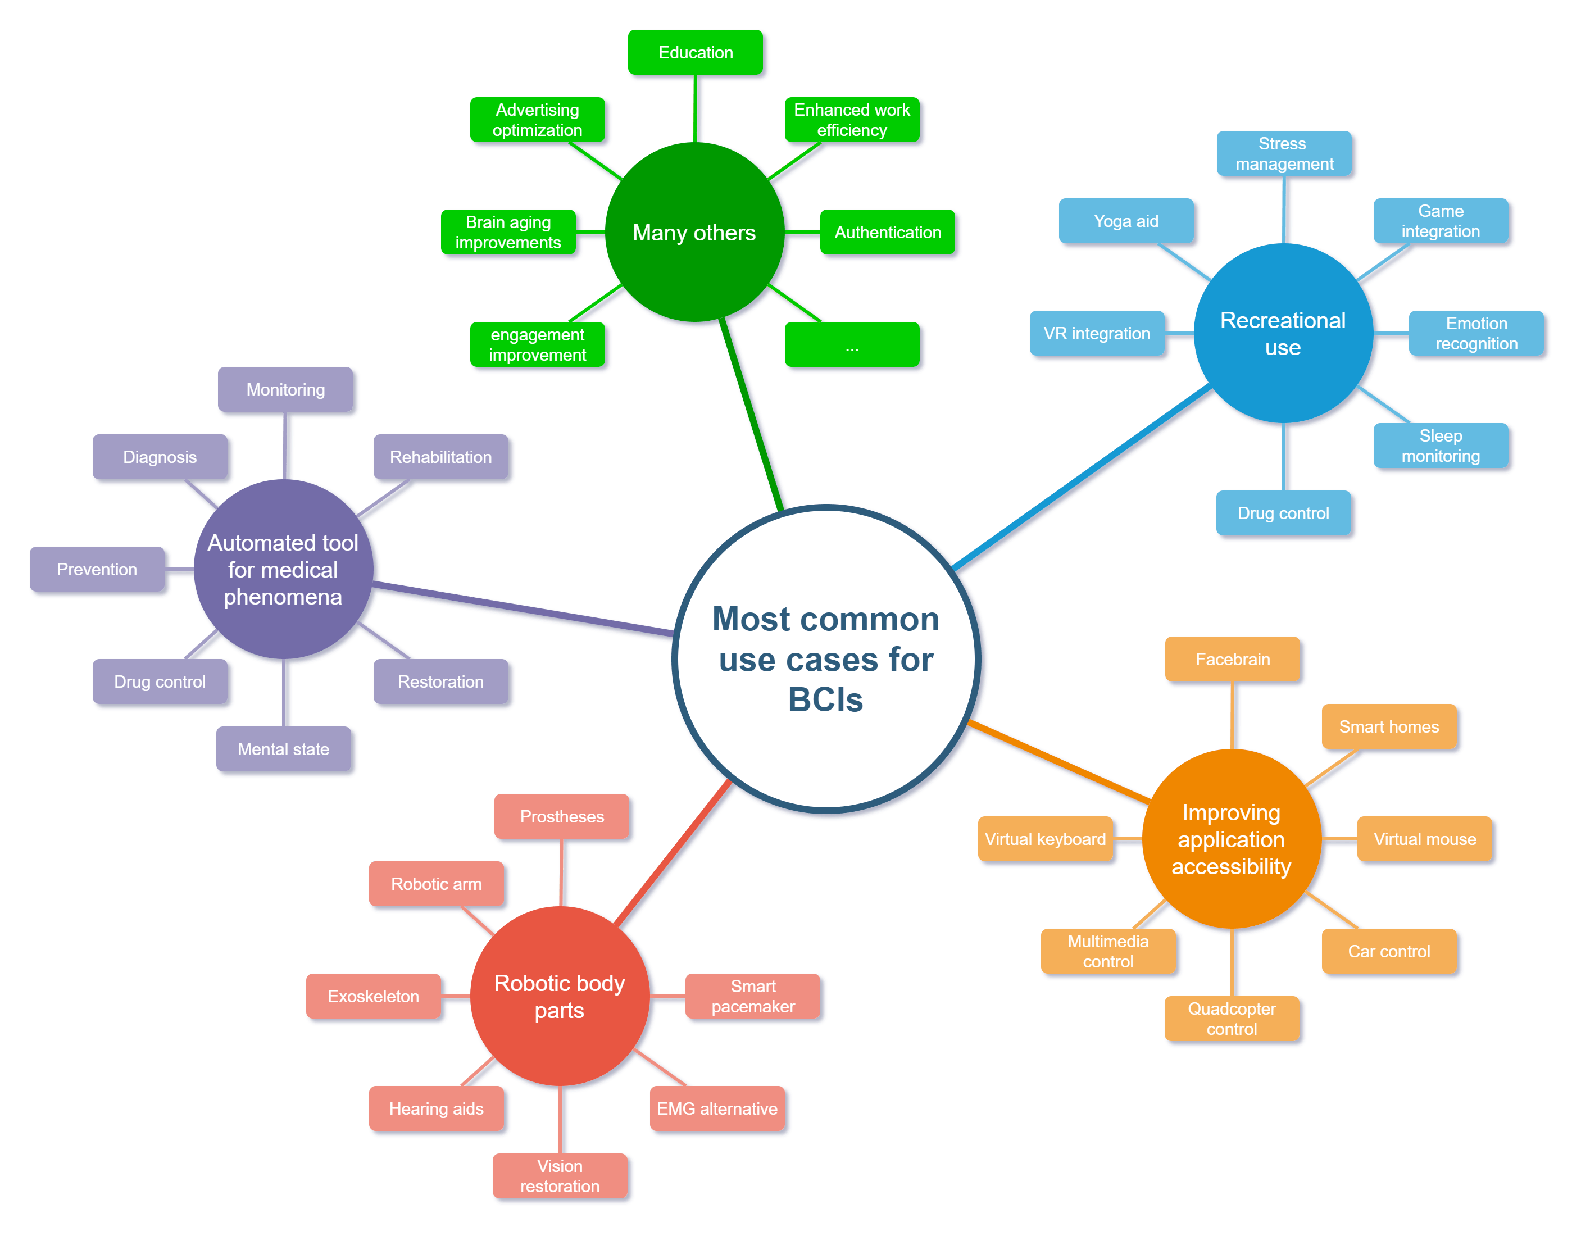
\includegraphics[width=\linewidth]{../images/introduction/use_cases_overview.pdf}
    \captionsetup{width=0.7\linewidth}
    \captionsetup{justification=centering}
    \caption{An overview of some of the many use cases for \glspl{bci}.} 
    \label{fig:bci_use_cases_diagram}
\end{figure}


% ---------------------------------------------- 
% Opportunities and obstacles for BCI research
% ---------------------------------------------- 

\section{Opportunities and obstacles for BCI research}
\label{sec:bci_opportunities_obstacles}

The most likely factors of why \glspl{bci} are gaining popularity and what the most common use cases are for \glspl{bci} were already discussed in Section \ref{sec:bci_gaining_popularity} and \ref{sec:bci_common_use_cases} respectively.
From these sections, an interested reader could have already spotted some opportunities and potential obstacles for doing research in the field themselves.
This section discusses some opportunities and obstacles present according to the author of this paper.
The aspects that are covered in this section are oriented towards the interests of the author from this master's thesis and aim to explain why this master's thesis came to fruition.
They also lay the foundation to the proposed \gls{bci} \gls{bc} system of this master' thesis, which will be further discussed in Section \ref{sec:bci_concolusion_and_proposing_ours}.


% ---------------------------------------------- 
% Small projects
% ---------------------------------------------- 

\subsection{Seemingly small projects with huge impact}
\label{subsec:bci_opportunities_obstacles_small_projects}

As \glspl{bci} and other technologies become more commercially oriented, the main focus is often shifted to providing products that can be used by the masses to provide the highest possible revenue.
Whilst \gls{bci} research sees its foundation from the medical world and most of the current users are people with a certain medical condition, a similar shift is likely, especially for the larger projects funded by big-tech companies.
This isn't necessarily a bad thing for medical applications, since this doesn't mean academic research focusing on those people with a certain medical condition disappears, rather it becomes a smaller portion of all research in the field.
The new technology and knowledge commercial products deliver can directly contribute to academic research focusing on medical applications.
This may include cheaper and more capable measuring equipment, a more socially acceptable picture of \glspl{bci} aiding the aesthetic aspect of Wolpaw's definition for a perfect \gls{bci} and better performing classification algorithms.
It is also possible that a commercial \gls{bci} application which is meant as a novelty for most, is life-changing to some.

Take the evolution of live captions as a recent example from a different domain, it has found its way directly into the Android smartphone operating system.
Whilst initially implemented for users to enjoy video content in situations where they can't listen to the audio, people with hearing difficulties now have a direct way to enjoy more content too.
The push for autonomous cars will allow those that are traditionally unable to drive a car to finally enjoy the freedom a car can offer as well without being dependent on others to do so.
Object and scene recognition algorithms made for optimizing smartphone cameras can also be used as a way of describing what is on a photograph for those who have limited vision.

Likewise, as more people are exposed to complex medical and commercial applications, many individuals start to envision seemingly small applications that could have a major impact on them or people they know.
This has been the case with smartphone applications for a long time.
A colour picker app that uses the camera to describe the colour of the central pixel is something that can be implemented with very limited resources.
Yet, such an application has already proven to significantly aid people who have colour blindness.
For example, they may use this application to determine whether a banana is ripe or not, something they can't visually determine but is easy with a textual description of the colour.
For such small applications to be feasible, an abundance of open-source material to re-use existing code for operating the camera, getting a textual colour description of an RGB colour code and more is required.

This presence of open-source code has started to emerge for the \gls{bci} field as well, as discussed in Section \ref{subsec:bci_gaining_popularity_better_processing}.
Combined with publicly available \gls{eeg} dataset such as the one by \citet{eeg_data}, it has become possible for developers to work on a pipeline without needing the monetary investment in \gls{eeg} measuring equipment.
If desired, the affordable headsets by OpenBCI and others, further compared in Section \ref{subsec:biomedical_signals_measuring_equipment}, make it possible to have \gls{eeg} measuring equipment with good open-source libraries for well under 1000 euros.
This has made individuals such as the author of this paper excited to create a wide variety of smaller applications that could have impactful meaning to some very specific people.
Especially the possibility of regaining even the simplest form of mobility through some very basic controls derived from \glsfirst{mi} is what motivated the author of this master's thesis to study the field.


% - - - - - - - - - -
% motivating aspects
% - - - - - - - - - -

\subsection{Motivational aspects for this master's thesis}
\label{subsec:bci_opportunities_obstacles_motivating_examples} 

The discussed use cases from Section \ref{sec:bci_common_use_cases} were motivating examples for this master's thesis in themselves.
However, there are some specific articles and aspects from the field that have motivated the creation of this master's thesis which will be discussed in detail here.
These are mainly related to \glsfirst{mi} based \glspl{bci} working with affordable consumer-grade and non-invasive \gls{eeg} measuring equipment.
Whilst many articles have demonstrated the potential of such \gls{bci} systems, the lack of widespread adoption suggests there are still hurdles to overcome for them to become a reality.
When discussing these motivating examples, some of these hurdles will already be discussed, the main obstacles for \gls{bci} research are further discussed in later subsections.


% | | | | | | | | | | | | |

\subsubsection{Consumer-grade EEG measuring equipment has promosing potential}
\label{subsubsec:bci_opportunities_obstacles_motivating_cheap_hardware_promosing}

Section \ref{subsec:bci_gaining_popularity_better_measuring} and \ref{subsec:bci_gaining_popularity_better_processing} have already discussed the evolution of \gls{eeg} measuring equipment as a potential reason for the increased popularity of \gls{bci} research.
Multiple studies comparing different aspects of cheaper consumer-grade systems to the more traditional medical-grade \gls{bci} systems have already been done \citep{openbci_vs_medical, openbci_eeg_sensor_evaluation, dry_electrode_status, wet_dry_comparison_experiment, wireless_dry_vs_wired_wet}.
In general, cheaper systems work with dry electrodes at a lower electrode count and have a lower signal quality compared to medical systems.
This means the cheaper systems provide poorer data quality, resulting in a more difficult classification problem.

This raises the question if useful applications can be made using data from these cheaper systems.
One of the best-known providers of \gls{eeg} equipment is OpenBCI and their products are further discussed in Section \ref{subsec:biomedical_signals_measuring_equipment}.
This OpenBCI headset makes use of the Texas Instrument ADS1299 chip to convert the analogue signal of \gls{eeg} electrodes to a digital one.
Whilst affordable and widely available, it has been shown that this chip is comparable to far more expensive alternatives that have been used in the laboratory for years \citep{openbci_eeg_sensor_evaluation, openbci_vs_medical}.
However, a cheap consumer-grade system differs from medical systems in more areas than the general chip responsible for \gls{eeg} amplification and digitalisation.

Studies comparing the use of cheaper dry electors against medical wet electrodes have already been discussed in Section \ref{subsec:bci_gaining_popularity_better_measuring}.
Whilst the obtained results from these studies show the gap between both is shrinking but still present \citep{wet_vs_dry, dry_electrode_status, wet_dry_comparison_experiment}.
However, the experiments used for obtaining these results come from very controlled experiments in lab-like environments.
This is to be expected, as most comparisons aim to eliminate as many random factors as possible.
However, this means that these experiments don't give great insight into the real-life usability and applicability of these cheaper \gls{bci} systems.
Taking into account that none of the academic research discussed in the systematic review article by \citet{bci_review_arnau} makes use of such cheap systems hints that real-world usage of these systems remains hard.


% | | | | | | | | | | | | |

\subsubsection{Trainable motor imagery as input thoughts for the BCI system}
\label{subsubsec:bci_opportunities_obstacles_motivating_mi_tasks}

Section \ref{subsec:bci_common_use_cases_bcis_replace_eye_tracking} discussed P300 based \gls{bci} systems.
Whilst the P300 signal is relatively easy to detect and evoke, the discussed visual stimuli used, have many limiting factors.
Perhaps most limiting is that the user can not evoke the signal without requiring external stimuli.
This is undesired in several ways.
This external stimulus requires an additional system to be present, such as the flashing grid commonly used for visual P300 \gls{bci}, which adds to the cost and complexity of the system and limits portability.
A system where a person sits behind a flashing screen is also hard to call aesthetically acceptable, making it unsuitable for Wolpaw's definition of a perfect \gls{bci}.

Detectable signals that can be evoked voluntarily by the user are more interesting for most \gls{bci} applications.
Likewise, the process to evoke this detectable signal should be one that doesn't require physical movement so that it is applicable for users suffering from limited muscle control.
It should ideally also be a process that is invisible to those around the user, making it aesthetically ideal for Wolpaw's definition of a perfect \gls{bci}.
\Glsfirst{mi} is such a cognitive process and is often used for controlling \glspl{bci} and in other fields such as sports, psychology, music, medicine and education \citep{mi_uses}.
\Citet{mi_definition} defines the \gls{mi} process as follows:


\setlength{\epigraphwidth}{0.9\textwidth}
\epigraph{Motor imagery is a cognitive process in which a subject imagines that (s)he performs a movement without actually performing the movement and without even tensing the muscles. It is a dynamic state during which the representation of a specific motor action is internally activated without any motor output. In other words, motor imagery requires the conscious activation of brain regions that are also involved in movement preparation and execution, accompanied by a voluntary inhibition of the actual movement.}{\textit{\citet{mi_definition}}}

\Gls{mi} does have some drawbacks as well, mostly following from \gls{mi} being a cognitive process with no visual clues.
Firstly, explaining how to \textit{do \gls{mi} correctly} is a difficult task.
Whilst it can be trained, it has a far steeper learning curve to obtain pleasing results than the earlier mentioned P300 systems relying on \gls{erp}-based signals for example.
\Citet{mi_training_hard} describes this problem and tips for teaching \gls{mi} in greater detail.
The most general procedure of explaining the \gls{mi} task to a user consists of verbally explaining the \gls{mi} task.
This can be further supported by a physical example of the task that should be envisioned.
People with the capabilities of performing the envisioned task physically can also be asked to perform the task whilst simultaneously thinking about it as a first step too.
After this, a training procedure of the user performing the \gls{mi} task without physical movement starts.

This introduces the second problem, evaluating the users \textit{capability of doing \gls{mi}}.
Such an evaluation exists of two parts, a survey taken beforehand and feedback during or after training.
Multiple types of surveys have been proposed to determine beforehand if a person will be good in \gls{mi} tasks \citep{kviq, mi_survey_miqrs, mi_survey1, mi_survey2, mi_capability_review}.
Most of these surveys are empirically created and based on the found correlations between the answers given by participants and their performance on a \gls{mi} \gls{bci} for those participants.
However, correlation does not mean causation, and it has been the case that these questionnaires do poorly at predicting a survey respondent's capability of doing \gls{mi} in a detectable manner.
For example, \citet{cheap_bci_feasibility} found no statistically significant correlation between the KVIQ-10 score of participants and the found classification accuracy.
Thus, determining beforehand if a participant will have pleasant accuracy results beforehand through the KVIQ-10 questionnaire by \citet{kviq} wasn't reliable for the experiment by \citet{cheap_bci_feasibility}.
This is an issue, as knowing this information beforehand can give a potential buyer a better indication if the system would be fit for them or not.
Other surveys have been proven more successful at predicting \gls{mi} capability of a user but further research in finding a survey that is reliable at predicting a user's \gls{mi} skills is still required \citep{mi_capability_review}.
Besides this survey that is taken beforehand, evaluating the \gls{mi} tasks performed by a user is also not an easy task.
Most of the time, a model is trained or calibrated after obtaining training and test samples of the user performing the \gls{mi} tasks.
The accuracy of this trained model can then be used as an indication of how good the user is at the \gls{mi} task.
Alternatively, the user might be exposed to live feedback during data collection in the form of a visual or physical stimulus that indicates the \gls{bci} is detecting a specific \gls{mi} task.
Including live feedback has been proven highly beneficial in training \gls{mi}, although it makes the training procedure even longer \citep{mi_training_hard}.
As evaluation in this way is mainly empirical based on the obtained classification result, it is not uncommon to see varying ways of doing the \gls{mi} task between users.
Some might perform the \gls{mi} tasks by envisioning the task from a third-person perspective whilst others opt for a first-person perspective.
This introduces many variables in the data, causing a high variability between users and even between sessions of the same user.
Visualisation of the brain signals and their decoding might aid in guiding users to perform a more equal \gls{mi} task, reducing the variability of the data.
However, since brain signals are non-stationary and the visualisation techniques are limited, variability will always remain an issue.
Forcing a user to perform the task in a specific manner also has downsides.
Their personal accuracy for the \gls{bci} system may be poorer when forced to do the \gls{mi} task in a very specific way compared to finding the optimal method for them.
The psychological burden of the long \gls{mi} training process will also be higher if the task is very strict, requiring more focus.
Finally, the data may be so strictly obtained that it is far from realistic and the system performs well in the real world.

This highlights the third and final important issue with \gls{mi}, the issue of generalisation.
This issue is present in two different forms.
First, there is the general issue not strictly limited to \gls{mi} that training and testing data is often obtained in strict manners and thus lab-like.
When used in the real world, more noise is present in the signal resulting in far poorer results.
The trained system does not generalize well to new, unseen data from the real world.
Second, as discussed the brain signals produced during \gls{mi} tasks can vary greatly between participants and sessions.
This variability means that creating a general model is far less successful, the trained model does not generalize well to other users.
This makes \glsfirst{tl} far more difficult.
This issue cascades to making the training procedure longer and having higher inter-patient variability in terms of accuracy results \citep{cheap_bci_feasibility, mi_training_hard}.
The generalisation issue is an important one in many \gls{ml} applications and is discussed further in Section \ref{subsec:processing_signals_common_issues_generalisation}.

These issues with \gls{mi} result in datasets that seem comparable from a high-level description of the performed \gls{mi} task but are very different in the used training procedure and data acquisition process.
The general \gls{mi} capabilities of the participants can also differ greatly between datasets, with some performing a survey beforehand to only include participants with a high possibility of being good at \gls{mi}.
This means that choosing datasets from \textit{well capable \gls{mi} performers} will result in higher accuracy scores as the data is easier to learn from.
Even when open-source databases are re-used between articles, it is not uncommon to find articles where the authors left out certain data in the training and testing procedure, arguing these users had poor \gls{mi} capability.
This makes a comparison of results between articles far more difficult.
This is an issue of not having standardized testing, which will be discussed in Section \ref{subsec:bci_opportunities_obstacles_lack_of_testing}.


% | | | | | | | | | | | | |

\subsubsection{Detailed literature on MI pipelines}
\label{subsubsec:bci_opportunities_obstacles_motivating_examples_mi_pipeline}

Section \ref{subsec:bci_gaining_popularity_improved_data_processing} discussed the emergence of more open-source datasets and code-providing libraries for \gls{bci} research.
However, many articles still fail to provide their source code and lack the required detail to fully recreate the used pipeline.
This makes articles describing their pipeline and design decisions in great detail stand out.
In general, these articles don't aim to improve the state-of-the-art in any component of the pipeline.
Rather, they contribute to the field by providing a detailed look at the working of pipelines based on available state-of-the-art solutions and a correct evaluation of them.

The article by \citet{cheap_bci_feasibility} discussing the feasibility of a complete low-cost consumer-grade \gls{bci} system is one that focuses on these aspects.
\Citet{cheap_bci_feasibility} performed their feasibility study by discussing the steps required to make an offline binary \gls{mi} classification system using common low-cost consumer-grade hardware.
The \gls{bci} distinguished two cases, the \gls{mi} task of a grasping movement with the participants' dominant hand and a rest condition.
They compare three traditional \gls{ml} approaches for this classification task in growing complexity.
These approaches differ in the feature extraction used, namely the use of traditional \gls{csp} and that of two extension, \gls{pfbcsp} and \gls{ptfbcsp}.
The work by \citet{cheap_bci_feasibility} has five interesting aspects worth highlighting here.

First, whilst they did use the consumer-grade OpenBCI Cyton and Daisy board they did not use the 3D printable Ultracortex Mark IV headset from OpenBCI.
They argued that this is due to the Ultracortex Mark IV headset becoming uncomfortable quickly due to the use of dry electrodes combined with limited adjustability.
This complaint on user comfort for the Ultracortex Mark IV headset is recurring with other authors including the one from this master's thesis.
Because of this, they opted for wet EEG electrodes attached to a very flexible and far more comfortable Electro-Cap.
\Citet{cheap_bci_feasibility} opting for wet electrodes is slightly odd, as it is not really consumer-grade nor does it fit well with Wolpaw's definition of a perfect \gls{bci}.

Secondly, for the data gathering of their system, \citet{cheap_bci_feasibility} used a \textit{common office room}, rather than a lab-like environment.
Except for a 3D printed holder for the OpenBCI board, there was no specialized shielding in place to protect the electrodes or OpenBCI boards from unwanted interference.
They argue this makes the data more realistic.
Whilst this is true to a certain extent, it is important to note there is still far less stochasticity than there would be in real life.
The office room and hardware were identical for each of the participants in the data collection stage.
The room was free of external stimuli with the participant \textit{left alone} to focus on the task and the task only during the entire trial.
All participants were right-handed and thus the dominant hand used for the \gls{mi} task was always the right hand.
Adding to all of this, the dominant hand of the participant was placed inside a box to not allow them to see their hand.
This makes the data acquisition procedure used by \citet{cheap_bci_feasibility} far from comparable to a real-world use case.
Still, \citet{cheap_bci_feasibility} found that the non-shielded regular office already caused significant noise compared to full lab settings.
In one trial the electromagnetic noise amplitude was four times higher than the meaningful EEG data.

Third, during the data collection, an \gls{emg} system was also in place.
This \gls{emg} system was used to filter out samples of the collected \gls{eeg} data where the envisioned movement was also physically performed, meaning it wasn't true \gls{mi}.
Whilst this forms an interesting and automated approach to data filtering when collecting training samples, the supplemental hardware that is only used during the training phase is probably a tough sell in a commercial application.

Fourth, they used the KVIQ-10 questionnaire by \citet{kviq} to determine how good a participant would be in \gls{mi}, a task that is proven to be harder for some individuals.
As discussed earlier, the results of these surveys are not reliable and only give a rough indication with many exceptions and surprising results possible.

Finally, even though the data acquisition happened under guidance in the work of \citet{cheap_bci_feasibility}, there were still issues with the recordings.
Out of the 12 participants, there were multiple moments where connection loss with the OpenBCI main board occurred and for one participant a defect rendered the data useless.
These issues are probably related to the quality of the consumer-grade hardware.
Part of the reason medical-grade hardware is about 5 to 10 times as expensive for a similar experiment is due to the strict certification medical-grade \gls{bci} should comply too.
This certification guarantees some form of quality and reliability from which it is expected connection issues and defects wouldn't appear as frequently.
Besides this, for one participant there were \gls{emg} detected movements of the hand for more than half of the \gls{mi} tasks rendering the trial of that patient useless as well.
Whilst this is an issue independent of the hardware used, it does indicate that learning how to do \gls{mi} requires training which takes time and effort.

To conclude, the work by \Citet{cheap_bci_feasibility} discusses the creation of a complete low-cost consumer-grade \gls{bci} system.
This system consists of the OpenBCI measuring equipment where the dry electrodes on the 3D printed Ultracortex Mark IV are replaced with electrodes in a more comfortable Electro-Cap.
The effective classification of the system is a binary \glsfirst{mi} classification on whether or not the participant imagines a grasping movement of the right, dominant hand or not.
\Citet{cheap_bci_feasibility} achieved an average accuracy between 70\% and 85\%, scaling with the complexity of the used \gls{csp} variation.
It is important to note that the evaluated models are on a patient-per-patient basis.
This means that each patient has their own uniquely trained model and that data from the same patient is used in the evaluation process.
Whilst the binary nature of the system makes it hard to find viable real-life applications, the performance reached is almost identical to those of medical-grade systems and follows from a slightly less lab-like environment than is typically the case.
The system proposed by \Citet{cheap_bci_feasibility} is of less importance in their work, rather the steps and pitfalls highlighted are of value.



\subsubsection{Detailed literature on complex classification pipelines}
\label{subsubsec:bci_opportunities_obstacles_motivating_examples_mi_models}

% TODO: herlezen met mogelijks meer/betere refs naar onze implemented models en discussion van die models zoals visualisation techniques etc

The above discussed article by \citet{cheap_bci_feasibility} provides great insight on the steps required to develop an \gls{eeg}-based consumer-grade \gls{bci} which uses \gls{mi} related signals.
Since \citet{cheap_bci_feasibility} uses a binary classification model, there are only two possible outputs of the classifier, which is too limited for most applications.
However, when working with \glspl{bci}, a lack of training samples combined with noisy and often high-dimensional data makes multi-class classification considerably harder than binary.
That being said, spatial filters such as the \gls{csp} approach and its extensions used by \citet{cheap_bci_feasibility} have been extended to support multi-class feature extraction.
The articles by \citet{eeg_mi_model_lda_csp, eeg_mi_model_deep_cnn_spatial_filters} have also studied the use of spatial pattern techniques for feature extraction.
This is done in combination with traditional \gls{ml} classifiers and \gls{dl} ones, both with promising results.

Many other multi-class classification pipelines have been proposed in literature that work well with \gls{mi} related \gls{eeg} data \citep{fbcnet, eeg_mi_model_mussi, eeg_mi_model_lda_csp, eeg_mi_model_deep_cnn_spatial_filters, eeg_mi_model_image_based, eeg_model_fbcsp, eeg_model_hbm, eeg_model_esi, eeg_model_eegnet}.
These proposed pipelines generally work on both consumer-grade and medical-grade systems, although consumer-grade systems can often benefit more from pipelines with specific noise-reduction steps.
Some of the proposed pipelines also focus on providing a general model which has been trained on data from multiple users and has usable performance for unseen users.
Whilst such models have poorer performance compared to one trained for a specific user, they can be used as an initial model to allow the user to explore the possibilities of the \gls{bci} without having to undergo the often tedious training data collection process.
Such a general model can also be used as a base model for calibration, a process based on the idea of \glsfirst{tl} further discussed in Section \ref{subsec:processing_signals_alternative_calibration}.

A complete in-depth review of all of the different approaches that have been proposed for \gls{eeg} classification falls outside the scope of this research paper.
\Citet{eeg_analysis_methods_epilepsy_review} compared \glsfirst{lr}, \glsfirst{ann}, \glsfirst{svm} and \glsfirst{cnn} for a binary classification task of either being epileptic \gls{eeg} data or not.
Whilst this is a binary classification task that is more tailored towards \glsfirst{cad}, the techniques used in the experiments are often used in the multi-class classification of \gls{eeg} data for common \gls{bci} purposes.
\Citet{eeg_analysis_methods_epilepsy_review} found that \glspl{ann} performed best for their classification task.
In general, \glspl{ann} and other \gls{dl} models such as \glspl{cnn} have proven to be more successful at \gls{eeg} data related tasks compared to traditional \gls{ml} approaches.

Because of this, many of the current state-of-the-art models for \gls{eeg} classification rely on \gls{dl} models.
Especially classification pipelines that include \glspl{cnn} have proven to be successful for \gls{eeg} classification \citep{fbcnet, eeg_mi_model_mussi, eeg_mi_model_deep_cnn_spatial_filters, eeg_model_hbm, eeg_model_esi, eeg_model_eegnet}.

The \gls{cnn}-based approach by \citet{eeg_model_hbm} is commonly regarded as current state-of-the-art for \gls{mi} classification.
The article by \citet{eeg_model_hbm} includes two different models, a deep \gls{cnn} named \text{DeepConvNet} and a shallower one named \text{ShallowConvNet}.
In Chapter \ref{ch:offline_bci_system}, both of these models will be implemented and discussed further.
\Citet{eeg_model_hbm} also describe a method of extracting a visualisation of the used brain signals by the model, which can aid in the explainability and interpretability of the model.
Explainability and interpretability are further discussed in Section \ref{subsec:processing_signals_common_issues_exaplainable}, Chapter \ref{ch:offline_bci_system} further addresses the visualisation technique.

One issue with more complex \gls{cnn}-based pipelines such as the DeepConvNet variant by \citet{eeg_model_hbm}, is the time and computational resources it takes to train the model and do predictions with it.
The latter is an issue for real-time classification, something that is needed for an online \gls{bci} system which often works with relatively low-powered computational units.
Pipelines such as the one by \citet{eeg_model_eegnet} have been developed to use \glspl{cnn} in such a way that real-time classification is possible.
The model proposed by \citet{eeg_model_eegnet} also has promising results and will also be implemented in Chapter \ref{ch:offline_bci_system} where it is discussed in greater detail as well.

Whilst \gls{cnn}-based pipelines are among the most popular for the classification of \gls{mi} \gls{eeg} data, they fail to use a fundamental aspect of \gls{eeg} data.
\Glspl{cnn} are not designed to perceive the input data as sequential data, which \gls{eeg} data is.
As such, they do not explicitely use this property of the data for learning.
\Glspl{rnn} and \glspl{lstm} in particular are a type of \gls{dl} networks that do explicitely use internal memory to explicitely use the sequential property for learning, as Section \ref{subsec:processing_signals_ml_and_dl_dl_classifiers} will discuss in greater detail.
These approaches are most popular in speech processing as it is the sequence in which words are spoken that gives meaning to a sentence rather than individual words.
\Citet{lstm_mi_eeg} used a traditional \gls{lstm} pipeline for \gls{mi} \gls{eeg} data classification with satisfactory results whilst \citet{lstm_cnn_mi_eeg} combined both ideas from \glspl{cnn} and \glspl{lstm} into a singular network that rivals \gls{cnn}-based state-of-the-art for \gls{mi} \gls{eeg} classification.

Some more noteworthy \gls{mi} related \gls{eeg} classification approaches include the one by \citet{eeg_mi_model_image_based} and the one by \citet{eeg_model_esi}.
\Citet{eeg_mi_model_image_based} took an interesting approach by first visualizing \gls{eeg} data as an image and using techniques from image processing for classification.
This yields decent results but doesn't reach the same level as the discussed state-of-the-art models.
However, the approach by \citet{eeg_model_esi} which incorporates the technique of \gls{esi} has shown to be as good or even better than state-of-the-art in specific experiments.



% | | | | | | | | | | | | |

\subsubsection{Connecting the classification model to physical devices}
\label{subsubsec:bci_opportunities_obstacles_motivating_examples_physical_devices}

As was discussed in Section \ref{sec:bci_introduction}, there is no exact definition of a \gls{bci}.
In general, a complete \gls{bci} system is seen as a combination of three different processes: a data collection process, a data processing step and a step where effective actions are taken by the \gls{bci} based on the processed data.
It is this last process that forms some ambiguity in what can be considered a \gls{bci} and what can't be, as was already discussed in Section \ref{sec:bci_common_use_cases}.
\Glspl{bci} that functions as \gls{bc} systems, which explicitely control an external device in real-time, are included in each definition of a \gls{bci}.
However, how such an external device is controlled can vary greatly and requires special attention which may influence all other components of the \gls{bci} as well. 

The labels provided by the classifier can be seen as an incoming input stream for the process responsible for mapping those classifications to an action on the external device.
When using \gls{mi} \gls{eeg}, it is intuitive to link the envisioned task with a similar action on the external device.
For example, an envisioned left-hand squeeze corresponds to a left movement whilst an envisioned right-hand squeeze corresponds to a right movement.
However, nothing is stopping the implementer from doing this mapping differently and in some scenarios, a less intuitive mapping might provide a more reliable and capable system that is easier to use.

This follows from some of the challenges with \gls{mi} \gls{eeg} classification, in particular a limited amount of output classes and the fact that it is easier to distinguish between major \gls{mi} tasks such as left-hand and right-hand movement rather than individual finger movement for example.
Since classification accuracy should be sufficient to operate the external device safely and reliably, a limited number of different and easy to distinguish \gls{mi} tasks are often used.

To illustrate how such limited classes can be used for effective \gls{bc} systems, imagine the movement of a robotic arm to pick up objects using \gls{mi} \gls{eeg} data through a classifier that can distinguish 4 \gls{mi} tasks: left-hand squeeze, right-hand squeeze, foot movement and an idle state.
Intuitively, one might want to obtain complete control over the robotic arm but the limited \gls{mi} tasks render a direct mapping between the classification label and all possible movements of the arm impossible.
The most intuitive solution is the creation of a menu for movement options as illustrated in Figure \ref{fig:example_arm_control_bad}.
Using the foot \gls{mi} task, the user switches between 3 operation modes of the robot arm: horizontal movement, vertical movement and grasping movement of the hand.
Dependent on the active menu, the left-hand squeeze and right-hand squeeze \gls{mi} tasks can be used to move the robot arm left and right, up and down or to open and shut the robot hand.
This provides the user with all available control whilst remaining relatively intuitive.
However, this assumes all commands are interpreted correctly.
When taking into account that state-of-the-art struggles to reach an average of 80\% accuracy for classifying four \gls{mi} tasks in favourable conditions, it is not unreasonable to think that best case there will still be a misclassification once every five steps on average \citep{four_class_mi_CSP_good, four_class_mi_hybrid_good, four_class_mi_klrrm_good, four_class_mi_wavelet_good}.
Taking into account that for picking up the desired object, the robot arm needs to be perfectly aligned both vertically and horizontally and the user needs to switch to the menu for grasping through envisioned foot movement and then chose the desired grasping movement through envisioned hand movement, it is highly unlikely this sequence of events will happen without misclassification.
This long sequence will not only make the system inefficient to use, but it will also expose one user's intention to more points of failure as it will require many steps.

Stepping away from the idea of wanting to control every movement of the robotic arm, a huge improvement in the efficiency of the system can be made.
With grasp detection algorithms such as the one proposed by \citet{graspnet}, the detection of objects of interest for the robot arm to interact with can be detected through computer-vision algorithms.
Using such algorithms, another way of controlling the robotic arm could rely on only three \gls{mi} tasks: left-hand squeeze, right-hand squeeze and an idle state.
Using the left-hand squeeze \gls{mi} task, the robot arm could be alternated between all possible items to grasp as detected by the grasp detection algorithm. 
Using the right-hand squeeze \gls{mi} task, the item could be picked up or set down depending on the current state and computer-vision-aided tools.
This limits the amount of successful consecutive steps needed and being a three class \gls{mi} classification, the accuracy is expected to be higher.
Thus, the system would be less intuitive but far more usable.
This proposed design is shown in Figure \ref{fig:example_arm_control_good}.
When comparing both subfigures of Figure \ref{fig:example_arm_control}, it becomes apparent that the less intuitive system is far more efficient at the given task, requiring only two actions to pick up the second glass rather than 13.
It is noted this is only an educational example and real systems would likely still require a more complex interface.
It is also noted that it is common to reduce misclassification by basing the taken actions on multiple classifications rather than one.

\begin{figure}
    \centering
    \begin{subfigure}{\textwidth}
        \centering
        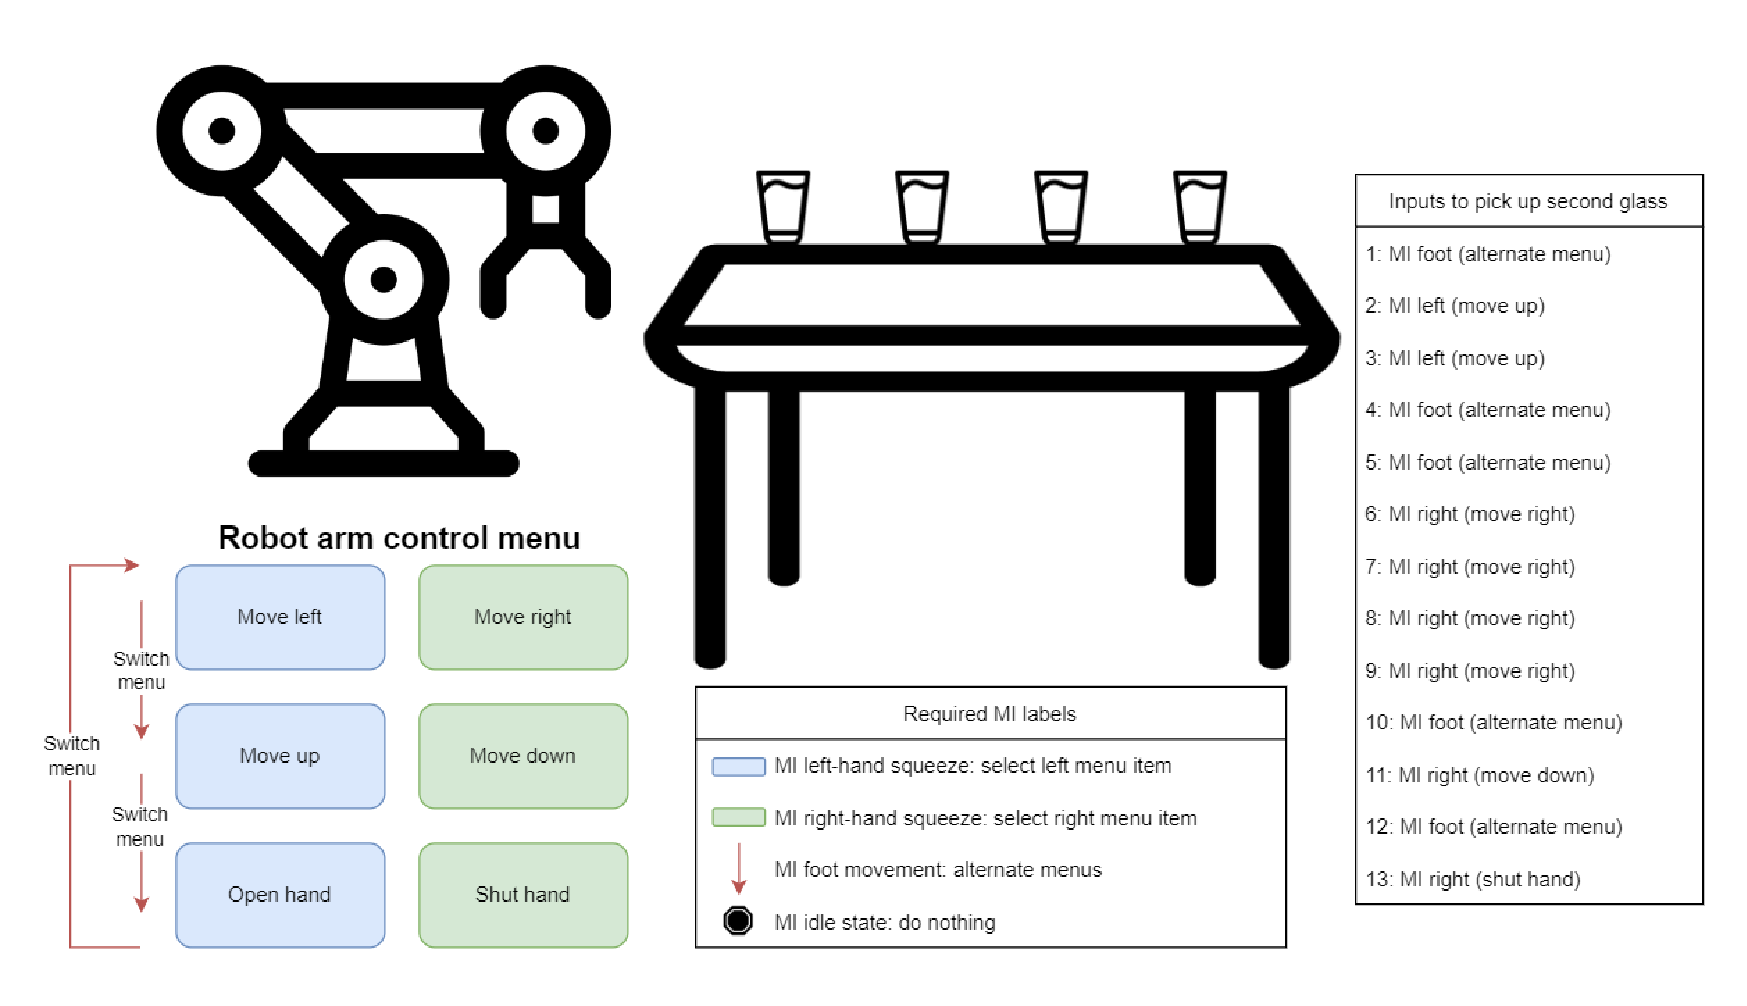
\includegraphics[width=\textwidth]{../images/introduction/example_arm_control_bad.pdf}
        \captionsetup{width=0.95\linewidth}
        \captionsetup{justification=centering}
        \caption{A \gls{bci} system that offers complete control over a robotic arm but with poor efficiency.}
        \label{fig:example_arm_control_bad}
    \end{subfigure}
    \hfill
    \begin{subfigure}{\textwidth}
        \centering
        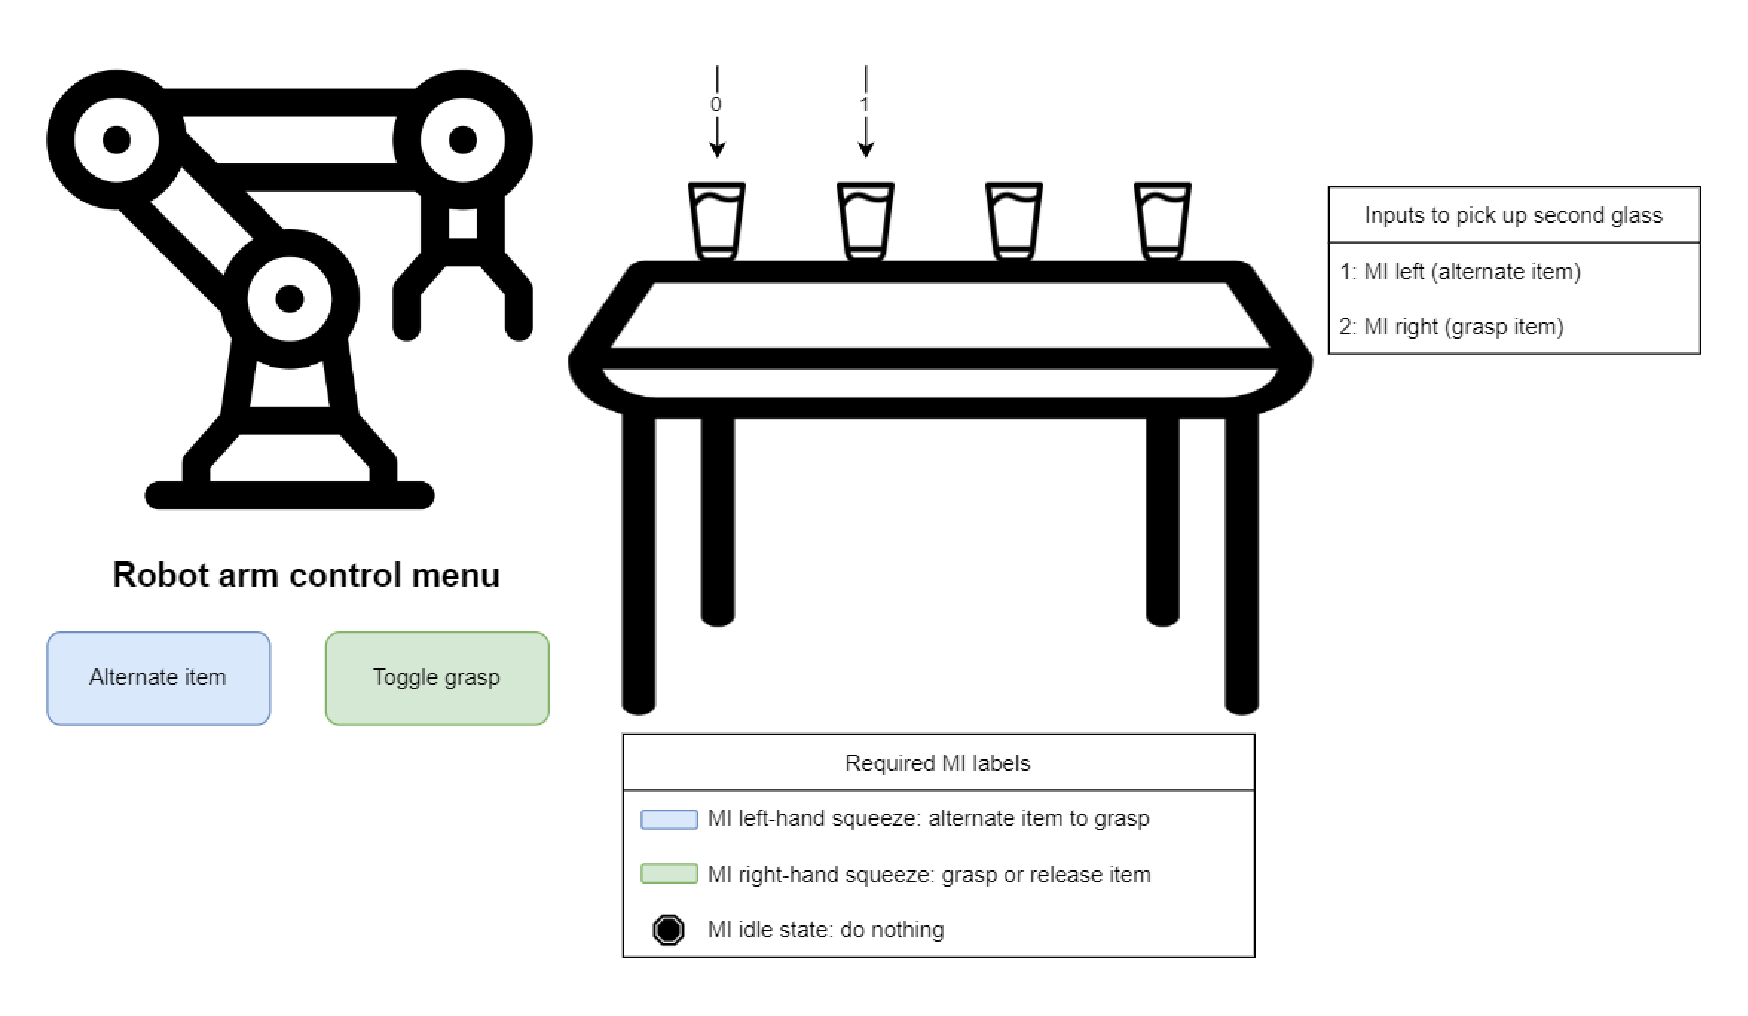
\includegraphics[width=\textwidth]{../images/introduction/example_arm_control_good.pdf}
        \captionsetup{width=0.95\linewidth}
        \captionsetup{justification=centering}
        \caption{A \gls{bci} system that offers limited control over a robotic arm but with great efficiency. \\ \hfill}
        \label{fig:example_arm_control_good}
    \end{subfigure}
    \captionsetup{width=\linewidth}
    \captionsetup{justification=centering}
    \caption{The contrast between mappings of \gls{mi} \gls{eeg} for controlling a robotic arm to grasp an item. One approach allows for full control but requires four \gls{mi} classes and many steps. One approach offers less control but succeeds in the task with three \gls{mi} classes and very few steps.}
    \label{fig:example_arm_control}
\end{figure}



\Citet{bci_mi_robot_arm} use comparable reasoning to propose a \gls{mi}-based \gls{bci} system to control a robot arm.
\Citet{bci_mi_robot_arm} use only three distinct \gls{mi} classifications: imagined right-hand movement, imagined left-hand movement and imagined foot movement.
These three controls enable the user to select eight different possible actions through a menu where two options are always shown that can be controlled using either an imagined left-hand movement or an imagined right-hand movement.
Scrolling through the menu to show two other possible actions is possible through the imagined foot movement.
This shows that with the right system design, few controls can still allow for many actions to be taken.
However, they lack a detection of the idle state.
This is possible by determining the idle state based on the certainty of the model that a certain prediction is correct.
If the model is uncertain, it is likely the user wasn't performing any of the \gls{mi} tasks and thus the system should not do anything.


% - - - - - - - - - -
% automated learning
% - - - - - - - - - -

\subsection{The potential of an AutoML variant for BCI pipelines}
\label{subsec:bci_opportunities_obstacles_automl}

People that are first introduced to \glsfirst{ml} and especially \glsfirst{dl} might think that these techniques provide a \textit{one-click solution} for data classification.
Whilst in some cases, re-using existing complex \gls{dl} methods can give satisfying results when providing it with enough training data, creating high-quality \gls{ml} and \gls{dl} systems still requires a lot of human expertise.
However, attempts are being made at providing such one-click solutions through a process called \gls{automl}, which is reviewed in detail by \citet{automl}.
The idea behind \gls{automl} is self-explanatory.
Rather than having an expert design a \gls{ml} pipeline, an automated system tries all sorts of combinations for a pipeline based on provided labelled data and perhaps some general preferences in techniques to be tested.
The problem then boils down to an optimisation problem where the combination of fine-tuned components that maximizes a certain metric such as accuracy on test data has to be found.
\Gls{automl} facilities have not yet been made for \gls{bci} specific pipelines, but with Google providing \gls{automl} as part of their cloud infrastructure for computer-vision, the \gls{automl} idea is becoming more and more popular \citep{bci_review_arnau}.

% | | | | | | | | | | | | |

\subsubsection{One library to develop a complete BCI pipeline}
\label{subsubsec:bci_opportunities_obstacles_automl_one_library}

When taking into account the discussed literature so far, it is clear that many techniques for each component of the \gls{bci} pipeline already exist and that certain combinations have proven to be very successful.
With more and more of these components being provided through open-source libraries as discussed in Section \ref{subsec:bci_gaining_popularity_improved_data_processing}, it is not unreasonable to think that an \gls{automl} library for \gls{bci} pipelines might be introduced in the future.
If done right, this pipeline can set standards for the expected output of each component meaning that newly proposed components can be directly provided to the framework by the author of that new component.
Whilst this would require a lot of commitment from the authors in the field, it could lead to newly gained insight on uncommon component combinations that provide a pipeline which performs best for certain problems.
Such a framework would also enable new research to re-use existing components much faster as they would ideally all be present in the library with some form of a standardized output.

As this library would require a lot of maintenance, it should be provided by a team that has sufficient resources on maintaining it and updating it to support newer techniques in the field.
Whilst there is currently no big organisation in the field that is likely to take this task upon themselves, the rise in popularity might attract such big corporations.

% | | | | | | | | | | | | |

\subsubsection{One library to develop multiple variants of one component from the BCI pipeline}
\label{subsubsec:bci_opportunities_obstacles_automl_one_component}

Besides aiming to provide a complete pipeline, a library that focuses on providing all alternatives of one component following a specific standard would already be incredibly handy.
Take for example a library that provides all open-source \gls{bci} datasets from one singular library, with all of the datasets following a specific standard.
This would allow for testing a model on a whole suite of \gls{bci} data, such as \gls{mi} \gls{eeg}, and thus make it easier to compare results with existing literature as these would also use datasets from this common library.
This has already been proven possible in other fields.
For example, in \glsfirst{rl}, the environments used for training, which could be seen as the training data, are often environments provided by the OpenAI Gym library \citep{gym}.
This library is maintained by OpenAI, a big company interested in \gls{rl} among other \gls{ai} techniques.
Due to its popularity, many other authors contribute to this open-source library by providing their custom environments in a format that is directly supported by the OpenAI Gym library.
A similar system for providing all sorts of \gls{bci} data would be incredibly helpful for the field of \gls{bci} research.
It could also cause a chain reaction, with the introduction of other libraries that include state-of-the-art classification algorithms which work directly with this common data-providing library.
This is also the case in the \gls{rl} field with libraries providing algorithms for these mentioned Gym environments \citep{tianshou, rllib}.
Thus, providing such a library as the first step to an \gls{automl} revolution in the \gls{bci} field might be a good idea.




% - - - - - - - - - -
% testing issues
% - - - - - - - - - -

\subsection{A lack of standardized testing and reporting}
\label{subsec:bci_opportunities_obstacles_lack_of_testing}

The evaluation and comparison of different \gls{bci} systems is not an easy task.
This is in part due to the many components a \gls{bci} system consists of, making direct comparisons often impossible.
Is comparing the performance of a classification model from a \gls{bci} system that works with dry electrodes in a real-world setting to one that works with data from medical equipment in a lab environment fair?
Is it fair to compare traditional two-step \gls{ml} approaches that have great explainability and interpretability with black-box one-step \gls{dl} approaches?
Many more of these questions exist and they remain mainly unsolved for the \gls{bci} field.

% | | | | | | | | | | | | |

\subsubsection{The issue with individually evaluating BCI pipeline components}
\label{subsubsec:bci_opportunities_obstacles_lack_of_testing_individual_components}

One potential approach is evaluating each component of the \gls{bci} system individually.
However, whilst these may make comparisons between the different components easier, these individual metrics don't tell the whole story for the complete system.
To truly test the capabilities of a proposed \gls{bci} system in the real world, intensive user studies should be performed.
Even in its simplest form, such a user study should validate if the \gls{bci} system succeeds in its advertised tasks in both a timely and reliable manner that is pleasant to use for the target audience \citep{bci_review_arnau}.
It should also be compared to existing solutions to ensure that there is an added benefit compared to these alternatives for the user.
To avoid biases, these user studies should not only include enough participants but the participant group should also be heterogeneous.

Doing even the most primitive version of such a user study takes significant resources to perform.
As such, it is rather uncommon to see these user studies in the same paper that proposes a \gls{bci} system.
Initial articles of a new proposed \gls{bci} system often focus on providing only objective evaluation metrics of the classification system.
These objective measures include accuracy, sensitivity and specificity.
Simple \glsfirst{poc} experiments are sometimes also included in these initial articles but these are tested only on a small group of participants, which are often not from the target audience.
The earlier discussed system by \citet{eye_tracking_vs_p300_comparable} was user tested on able-bodied participants whilst the target audience was not.
As discussed in Section \ref{subsec:bci_common_use_cases_bcis_replace_eye_tracking}, this study gave promosing results while a comparable system tested for a person in the target audience found that the user wasn't interested in using the proposed \gls{bci} system as existing solutions were more pleasant to use \citep{no_interest_in_using_p300}.
Some of the articles included in the review by \citet{bci_review_arnau} also performed user tests on participants that are not part of the target audience.
However, with many current \gls{bci} systems focusing on providing systems for medical purposes, finding enough participants from the target audience to form a heterogeneous group can be challenging.



% | | | | | | | | | | | | |

\subsubsection{Proposing a complete BCI system throughout at least four articles}
\label{subsubsec:bci_opportunities_obstacles_lack_of_testing_four_articles}

The above-mentioned points make the author of this master's thesis believe that the development of a \gls{bci} system should take place over at least four separate articles.
The first article should focus on data acquisition.
It should discuss the equipment used for recording the brain signals.
It should also address which kind of brain signals are extracted and where they are expected to originate from on an anatomical level.
The exact procedure used for effective data collection should also be detailed.
This includes details on what participants are included, if there were surveys used to test their capabilities both before or after the experiments, if the participants were trained, how many trials over which periods were performed per participant and much more. 
Such an article may contribute to the field by providing an open-source dataset, describing a novel training technique, discussing a more user-friendly data collection procedure, proposing new hardware and more.
What kind of evaluation should be done in this type of article depends mainly on what the contribution of the article is.
When proposing completely new hardware, a comparison between comparable hardware may be done in the same manner as \citet{compare_eeg_devices_for_ssvep} compared different consumer-grade \gls{eeg} headsets.
When testing a new training procedure, the data may be fitted to a common classifier to compare its learnability with the data of participants that followed a different training procedure. 
Discussing all possible evaluation metrics falls outside the scope of this master's thesis, but the most important factor is discussing the exact data acquisition process, as important details such as if live feedback was used often lack in existing work providing open-source datasets.

A second article should focus on the classification pipeline.
It can contribute by proposing a novel combination of existing pipeline components or completely new components altogether.
The type of components such a pipeline has and the evaluation that can be done will be discussed in detail in Chapter \ref{ch:processing_signals}.
These articles will make use of the data from the first article on data acquisition and should thus briefly summarize the used dataset.
The experiments that will be done in this Master's thesis relate mainly to this type of article.

A third article should focus on linking this system to an external device such as a robot arm.
This might involve changes to the classification pipelines, especially in the cutoff values for specific classes.
Rather than optimizing global accuracy, it might be preferred to tune the system such that it makes more, but predictable errors.
To illustrate this, a pipeline might be tuned such that it has a high true positive rate and a low false positive rate for actions that have significant risk.
This means that when these actions with certain risks are performed, the system is almost certain the classification was correct.
Doing this will make more false classifications for the other classes, but if these classes are neutral classes that don't perform actions, it has less risk associated.
This corresponds to preferring a \gls{bci} for \gls{bc} over a robot arm that has a global accuracy of only 80\% but makes almost all of its errors in not moving when movement was desired over one that has 85\% global accuracy but has most errors in it moving when no movement was desired.
The focus of this article is not on obtaining the best classification metrics anymore but rather on providing the safest and most predictable system that is still useful.
This third article might perform a simple \gls{poc} to validate that the desired action taking is possible, even if this is only tested for best-case scenarios.
It can contribute to the field by proposing more intuitive interaction methods, a new form or external device, a clever way of boosting reliability and predictability and more.

A fourth article should then focus on an in-depth user study with a heterogeneous group from the target audience.
Ideally, this study should be performed over multiple sessions to study long-term impacts on the user's life, including an idea of the public acceptance of the proposed system.
It should review all previous articles and is likely to require most resources, but is also the most important for bringing the proposed \gls{bci} to the real world.
It contributes to the field by addressing the good and bad points of a proposed \gls{bci} system being used in the real world.
It may highlight points that went undetected in the previous articles. 

% | | | | | | | | | | | | |

\subsubsection{Comparing these different articles}
\label{subsubsec:bci_opportunities_obstacles_lack_of_testing_comparing}

Some metrics for comparing each type of article with each other were named in this section already.
However, standardized tests should be introduced to fully ensure comparability between results and that a correct evaluation is done in each article.
These are not yet present in the \gls{bci} field and proposing them is a difficult task as the proposing authors should be respected so that other authors are even willing to accept their proposals.
It is also not easy to propose testing and reporting standards that fit all variants of these proposed articles.
Do you train the models on a single patient and test them on the same patient or do you test for generalisability?
Do you allow it to run on very capable hardware or limited but very affordable hardware?
It should be apparent that there is no straightforward way of proposing standardized testing and reporting for all variants of these articles.

This master's thesis only aims to highlight these issues as solving them is an open issue and standardized methods would need the consensus of the field, which a master's thesis is unlikely to obtain.
For now, creating at least four different papers to propose a complete \gls{bci} system and focusing on being as transparent as possible in each is already a good step in the right direction.
However, transparency lacks in many papers, albeit due to page constraints or a lack of standardized reporting.
Providing the source code with additional notes through an external source such as GitHub may help combat the page constraint issue.
Following guidelines from related fields such as PROBAST  \citep{probast} and TRIPOD  \citep{tripod} originally proposed for \gls{cad} and \gls{cade} research can help in determining a new reporting standard for \gls{bci} research.
Such a reporting standard will also aid in the repeatability and reproducibility of articles, especially for those where sharing the source code and data is not possible.

% - - - - - - - - - -
% interdesciplinary issues
% - - - - - - - - - -

\subsection{Challenges from the highly interdisciplinary nature of BCI systems}
\label{subsec:bci_opportunities_obstacles_interdisciplinary}

The idea of splitting the development of a complete \gls{bci} system into at least four separate articles discussed in Section \ref{subsec:bci_opportunities_obstacles_lack_of_testing} can also help with the challenges that the highly interdisciplinary nature of BCI systems offers.
This is because each of those articles limits itself to a couple of domains rather than all domains present in \gls{bci} research.
In practice, many articles aim to provide a system that is as complete as possible but this results in a system where many components, that fall outside the knowledge domain of the authors, are adopted from previous literature providing little to no scientific value.

% | | | | | | | | | | | | |

\subsubsection{Disciplines needed for each of the four proposed articles}
\label{subsubsec:bci_opportunities_obstacles_interdisciplinary_four_articles}


When taking into account the four separate articles needed for proposing a complete \gls{bci} system proposed in Section \ref{subsec:bci_opportunities_obstacles_lack_of_testing}, the following experts may be required.
For the data acquisition article, a neuroscientist can greatly improve the value of the article by understanding in detail what brain signals can be measured and what interpretation they may have.
They can also help in determining the optimal placement of the electrodes based on the anatomy of the brain and the expected source of the signal of interest.
To create the hardware for the headset that captures the wanted brain signals, e.g. an \gls{eeg} headset, engineers capable of reliably measuring and transmitting these incredibly low voltage and noisy signals are needed.
A graphical designer can help with making the headset aesthetically acceptable.

The article related to data classification can be done mainly by a computer scientist specialised in \glsfirst{ml}.
However, when making visualisations and features, knowledge from neuroscience may still be needed.
Because of this, a neuroscientist may still be very helpful for this article.
Likewise, whilst a computer scientist may be able to reduce noise in a software manner, having an understanding of how the headset works and what types of noise and artefacts can be expected is also incredibly helpful.
Whilst a well-documented data acquisition article may cover all these points, some aid from engineers in understanding the headset hardware can still be helpful.

For the third article, where the connection to an external device is discussed, a wide variety of experts may be required.
For example, the previously discussed robotic arm with example menu's shown in Figure \ref{fig:example_arm_control} requires computer vision knowledge for grasp detection, engineering knowledge to make the robot arm and general computer science knowledge to create a working link between classification labels and action controls.
A graphical designer may once again help with making the external device aesthetically acceptable.
General \glsfirst{ux} knowledge can help in creating a great mapping between the detected brain signals and the control over the external device.


The fourth article may require all previous experts to finetune and configure the system.
Since these trials involve human participants and often people suffering from a handicap, an ethics expert should also be consulted.
Adding to this, by surveying the users in a manner that truly captures the \gls{ux} and net benefits, both a psychologist and an expert of comparable systems may be needed.
These discussed experts may vary greatly based on the type of \gls{bci} system that is proposed.

% | | | | | | | | | | | | |

\subsubsection{The issue with wanting to propose a complete system directly}
\label{subsubsec:bci_opportunities_obstacles_interdisciplinary_complete_system}

The idea of proposing a \gls{bci} system as a result of four articles is proposed in this master's thesis and is currently not present in the field.
Whilst some researchers do focus on some components of a \gls{bci} system only, in the same spirit the division in multiple articles would do, most researchers aim to also propose a complete working \gls{bci} system in terms of a \glsfirst{poc}.
Take for example the \gls{bci} system proposed by \citet{complex_hand_few_classes}.
It has a significantly sophisticated robotic hand that functions almost completely as a human hand does.
The effective hardware used for the complete \gls{bci} system, including the processing unit, are also well detailed.
This shows that the authors have a significant understanding of the hardware a \gls{bci} system requires.
However, the methodology used for data acquisition, the used classification algorithms and the user interface to the external system as proposed by \citet{complex_hand_few_classes} could benefit from improvements.
Since this is mostly a straight copy of existing methods and models not optimized to their proposed \gls{bci} system, one could argue they have little scientific value.
The simple \gls{poc} experiments are also of low value as discussed in Section \ref{subsec:bci_opportunities_obstacles_lack_of_testing}.
This means that these added components to create a \gls{poc}, which take significant time, have a limited scientific value.
This is by no means a criticism to \citet{complex_hand_few_classes} but demonstrates the interdisciplinary nature of \gls{bci} systems and how researchers that are specialized in one of these disciplines will outperform certain aspects of a \gls{bci} system while leaving room for improvement in other aspects.
This interdisciplinary nature of the \gls{bci} field is part of what makes it so fascinating yet also very sophisticated with a steep learning curve.
The above-proposed idea of splitting the development of a complete \gls{bci} system into multiple papers could limit the amount of time put into creating components that fall outside the scope of expertise and thus have less value in the article.


% - - - - - - - - - -
% repeatability issues
% - - - - - - - - - -

\subsection{Brain signals are a complex data source}
\label{subsec:bci_opportunities_obstacles_complex}


The human brain is an incredibly complex system of billions of neurons and trillions of synapses.
Whilst great efforts are being made in mapping all of these neurons and synapses, faster than predicted, a complete mapping remains unavailable.
The lack of such a complete mapping directly implies that research is unable to simulate the brain in silico.
It also implies that there are still many unknowns in the complete structure of the brain and its internal working.
\Citet{brainmapping} talks about the efforts in mapping the brain and the many unknowns still present in the working of the brain in more detail.
This limited understanding of the brain makes it a highly complex source of data, even when working with well-understood brain signals.

The most difficulties in using brain signals as a data source arise from the fact that the brain is a dynamic, nonstationary and non-linear system \citep{bci_applications}.
Non-linearity is a common challenge in many research fields and many \gls{ml} and \gls{dl} models can work with non-linearly correlated data.
However, the dynamic and nonstationary nature of brain signals is less common in applications of \gls{ml} and \gls{dl}.
Intuitively, this dynamic and nonstationary property results in measurements that can differ greatly for the same patient during the same trial doing the same task.
For example, an envisioned \gls{mi} task of the right-hand movement can be repeated by the user multiple times.
However, the user's mental and emotional state, their focus and fatigue levels and many other aspects that will influence the brain signals will change continuously.
Both due to the limited spatial resolution of measuring modalities and our limited knowledge of the brain, it is impossible to measure the wanted brain signal without measuring any other brain activity.
Thus, this change in the brain activity that is not of interest makes the measurements nonstationary and dynamic, making the learning task significantly harder and more complex.

Adding to this, neuroplasticity, which was already discussed in Section \ref{subsec:bci_common_use_cases_medical_phenomena}, can change the structure and working of the brain.
This makes the brain even more dynamic.
Adding to what could be seen as internal noise factors of the brain, external noise can also be present in a nonstationary and dynamic manner.
This external noise includes common artifacts such as electrical interference and the detection of \gls{emg}, which will be discussed in more detail in Section \ref{subsec:biomedical_signals_measuring_artefacts}.

All of these factors already makes brain signals an incredibly complex data source for \gls{ml} and \gls{dl}, as is used in \gls{bci} systems.
The limited knowledge of the brain's inner working and the dynamic, nonstationary and noisy nature of brain signal measurements also challenges the explainability and interpretability of these signals.
This issue of explainability and interpretability is further discussed in Section \ref{subsec:processing_signals_common_issues_exaplainable}.
Besides these factors, brain measurements are far harder to collect resulting in an often very limited amount of training data \citep{bci_applications}.
This makes many of the techniques used in fields where gigantic datasets are available, unapplicable for \gls{bci} research.
Take for example the \gls{eeg} \gls{mi} dataset by \citet{eeg_data}, which is one of the largest publicly available datasets of this type.
This dataset by \citet{eeg_data} has around 60 000 combined usable samples over many different \gls{mi} tasks and paradigms.
Taking into account that only a subset of these samples can be used for training, this collection is multiple orders of magnitude smaller than datasets from other \gls{ml} and \gls{dl} applications.
Take for example the commonly used ImageNet dataset by \citet{imagenet} which contains over 3 000 000 images for training an image recognition classifier.
The high dimensional and time-dependent nature of brain measurements also makes it harder to re-use common \gls{ml} and \gls{dl} approaches from other fields.



 




% ---------------------------------------------- 
% ETHICAL CHALLENGES
% ---------------------------------------------- 

\section{Ethical challenges for BCIs}
\label{sec:bci_ethical}

% plural full needed
\glsreset{bci}

The field of \glspl{bci} has many promosing aspects, with Sections \ref{sec:bci_gaining_popularity}, \ref{sec:bci_common_use_cases} and \ref{sec:bci_opportunities_obstacles} discussing the rise in popularity, the growing amount of use cases for \gls{bci} systems and some of the opportunities in the field.
These evolutions in the field have made \glspl{bci} present in more then just research labs \citep{ethical_dillemas,bci_applications}.
Widespread adoption of \gls{bci} systems is still unlikely in its current state, with some obstacles that need to be overcome first.
This relates to creating a system that fits Wolpaw's definition of a perfect \gls{bci} and overcoming at least the challenges discussed in Section \ref{sec:bci_opportunities_obstacles}.
However, with the recent news coverage of the Elon Musk company Neuralink \citep{neuralink_whitepaper}, discussed in Section \ref{subsec:bci_gaining_popularity_big_tech}, it has become clear that ethical challenges might be tougher to overcome than technical ones.
Even if Wolpaw's vision of a perfect \gls{bci} can be met and a net benefit to the user has been proven, some users' moral intuition may refrain them from using such a system.

Whilst the author of this Master's thesis is by no means an ethics expert, he believes that it is important for any researcher interested in the \gls{bci} field to be aware of some of the many ethical challenges \glspl{bci} have.
This section aims to illustrate what kinds of ethical challenges are related to \gls{bci} research and how there is no clear solution for them.
The interested reader is invited to consult the interesting articles on the ethics of \glspl{bci} by \citet{ethics_of_bci} and \citet{ethical_dillemas} for a more in depth ethical study.
Some articles have also been made focusing solely on ethical questions surrounding the Neuralink proposed \gls{bci} \citep{neuralink_ethics,neuralink_ethics2}.

% - - - - - - - - - -
% confrontation
% - - - - - - - - - -

\subsection{Painfully confronting users with their brain}
\label{subsec:bci_ethical_confronting}

When a \gls{bci} system is used by patients suffering from a brain disorder, it is easy for the user to be confronted with their disorder by that system.
Take for example an invasive medical \gls{bci} used to predict when an epileptic seizure would occur such that it can alert the user to take the right medication to prevent the seizure from occurring.
Each time the system alerts the user, the user is confronted with the fact that they have epilepsy and a potential epileptic seizure coming.
\Citet{first_bci_trial} performed a clinical trial on six users suffering from epilepsy that use such a \gls{bci} system.
Whilst positive results in seizure reduction were found for all patients using the system, the \glsfirst{ux} differs greatly between all six participants.

From all six patients, four expressed how they felt more in control of their daily life thanks to the system.
They reported a pleasant overall experience with the system.
Another patient, \textit{patient four}, expressed that he saw epilepsy as part of his life and himself.
As a result, he wasn't interested in being dependent on the \gls{bci} system to warn him and ignored it most of the time.
More worryingly, \textit{patient three} said the following: 

\setlength{\epigraphwidth}{0.9\textwidth}
\epigraph{[The BCI] made me feel I had no control. So I didn't have control over what I was going to do. [...]  It made me feel that I was always different [from] everyone not just in the moment of the seizure [...] I got really depressed}{\textit{Patient three from the study by \citet{first_bci_trial}}}

Being aware that the system was constantly monitoring her brain activity and an alert could be sent at any time, the patient felt \textit{different to everyone else} all of the time, whilst without the system, this feeling was only present when a seizure occurred.
The \gls{bci} system constantly reminded her that she has a brain condition which had a significant psychological burden.
Whilst this is only the experience of one patient from a small trial, it was an important finding that has given many ethicists reason to question the use of \gls{bci} systems for all patients \citep{ethics_of_bci}.
It is not unreasonable to think that similar feelings might occur when using \glspl{bci} for neurological rehabilitation through neuroplasticity, a use case discussed in Section \ref{subsubsec:bci_common_use_cases_medical_phenomena_restoration}.
Neuroplasticity may take a long time or even be impossible for some users.
Having constant feedback that shows no or poor progress can be very confronting for the user.
Even in commercial settings, when a person tries to calibrate a headset relying on \gls{mi} tasks and the calibration fails due to the user being poor in envisioning the \gls{mi} task, a feeling of \textit{lacking this capability compared to others} might cause a dramatic \gls{ux}.
This poor \gls{ux} for certain users is something that can only be found with thorough trials and further shows how important it is to do real-world experiments.

% - - - - - - - - - -
% e-waste
% - - - - - - - - - -

\subsection{E-waste inside your skull}
\label{subsec:bci_ethical_e_waste}

Section \ref{subsec:bci_common_use_cases_prosthesis_exoskeleton} already adressed Second Sight, one of few companies providing visual prostheses with approval from the \gls{fda}.
This company discontinued support for some of its earlier visual prostheses.
This resulted in all of the users from those early products losing any form of support.
As discussed by \citet{second_sight_broken_ethics}, this has major consequences.
First, the technology that has enabled them to restore their vision to a certain extent can fail at any time.
If this happens, this results in an indefinite loss of vision again due to the lack of support.
Second, the company refuses to make the required data for the maintenance of the system public.
This means that no third party can ever work on it.
Third, due to no third party being capable of removing the system, the users are essentially stuck with what is or will become e-waste inside their skull.
This has already caused major issues for one user, Ross Doerr.
As discussed by \citet{second_sight_broken_ethics}, Ross can't get the help he needs with a brain tumour due to doctors not having the required information about the brain implant to ensure a safe operation.
Even a simple \gls{mri} scan can't be planned safely due to this lack of information surrounding the brain implant.

With commercial companies showing interest in invasive \glspl{bci}, such as the earlier discussed Elon Musk company Neuralink, it is not unreasonable to think a similar situation might occur from the manufacturer of such systems.
What happens to an invasive \gls{bci} system once the manufacturer doesn't support it anymore or the patient isn't interested in using it anymore?
It becomes clear that some form of regulations should be in place to ensure that users of such invasive systems are always able to get the information needed from the manufacturer to ensure they are not restricted in getting needed care.
It also begs the question if invasive \glspl{bci} is really the road to go and how dependent we want to be on these technologies, taking into account they might fail for an unspecified period at some point.

% - - - - - - - - - -
% personal identity
% - - - - - - - - - -

\subsection{Changing peoples personal identities}
\label{subsec:bci_ethical_identity}

Section \ref{subsec:bci_ethical_confronting} already adressed the trial conducted by \citet{first_bci_trial}.
In this trial, six patients suffering from epilepsy using an invasive \gls{bci} for epileptic seizure reduction were monitored over a long period.
Besides the finding of extreme psychological burden for one patient, the following words from \textit{patient six} are also eye-opening:

\setlength{\epigraphwidth}{0.9\textwidth}
\epigraph{[The BCI] was me, it became me. [...] I found myself changing. [...] I felt like I could do anything. [...] With this device, I found myself. }{\textit{Patient six from the study by \citet{first_bci_trial}}}

Whilst this is a positive experience according to the user, \citet{first_bci_trial} described this as a radical symbiosis between the patient and the system.
The idea of users feeling themselves becoming one with technology, creating a symbiosis, has multiple ethical concerns \citep{ethics_of_bci}.
These concerns fall outside the scope of this small ethical discussion on \glspl{bci}.
However, this change of personality is something that can influence the patient's life in a manner that perhaps wasn't initially expected.
For example, when someone goes through major weight loss, they have more chance to see a marital status change.
Both in terms of getting married or having a divorce \citep{weight_loss_divorce}.
Similar trends might occur due to behaviour changes as a consequence of having a \gls{bci}.

Likewise, some people that suffer from a medical condition might embrace their condition and share some sort of culture with people that have the same condition.
People suffering from major hearing loss may enjoy parties oriented toward them where bass-heavy music is played at loud volumes such that they can feel the vibrations of the music throughout their body.
For them, this is how they can enjoy music without hearing music.
If such a person were to regain hearing through a \gls{bci}, it is unlikely they will enjoy hearing the load and constant bass.
Similarly, people suffering from major vision impairment might enjoy tactile art.
When vision is restored, their impressions of these kinds of artworks are bound to change.

In both of these situations, the interest in the events they once liked might faint and the connection to the community surrounding them might vanish.
They lose touch with the \textit{community they were once part of} (i.e. the blind and deaf community).
These are things that might go unthought of when looking at the added benefits of a \gls{bci} system might offer.
However, they can cause major identity issues where users are left in a quest of finding who they are after a major change in their daily life.
This quest is one that not many look forward to doing and maybe a reason some people opt to not use a \gls{bci} system.


% - - - - - - - - - -
% sloppy science
% - - - - - - - - - -

\subsection{A great risk of sloppy science}
\label{subsec:bci_ethical_sloppy_science}

With a lack of standardized testing and reporting as discussed in Section \ref{subsec:bci_opportunities_obstacles_lack_of_testing}, it is easy for researchers to perform \textit{sloppy science}.
It allows them to report and compare only those metrics that have the desired outcomes rather than performing time-consuming user trials that have the most scientific value.
With many authors wanting to propose complete systems over singular components, the risk of sloppy science is increased even further as the other components are highly likely to receive less thought resulting in poorer quality, as discussed in Section \ref{subsec:bci_opportunities_obstacles_interdisciplinary}.
However, respected journals have appropriate mechanisms in place, such as peer reviews, to stop published articles from performing sloppy science.

More worryingly, private companies aiming to commercialise their \gls{bci} systems as soon as possible are less subject to these mechanisms of protecting against sloppy science.
\Citet{tailored_brain_book} expresses some of her concerns with Elon Musk's Neuralink company in this regard.
\Citet{tailored_brain_book} refers to an interview with ex-employees by \citet{neuralink_rushed_timelines}.
In that interview, it is discussed how more than half of the initial researchers have left the Neuralink company already and how these ex-employees experienced a rushed timeline which wasn't compatible with the slow pace of science.
This led to multiple internal discussions between the initial researchers wanting more time and shareholders wanting a sellable product quickly.
Whilst these ex-employees were also quick to state that they see Neuralink as an incredibly innovative company in the \gls{bci} field and believe they will succeed in their mission, these words about a rushed timeline are worrying.
As discussed in Section \ref{subsec:bci_opportunities_obstacles_lack_of_testing}, thorough experiments take a lot of time, so it isn't surprising that this isn't compatible with a commercial aim of providing a product to market as soon as possible.
However, when considering that Neuralink's proposed system is an invasive one and the ethical questions about e-waste in your brain discussed in Section \ref{subsec:bci_ethical_e_waste}, the worry of such companies performing sloppy science to be among the first on the market only grows.
Whilst some legislations are in place that should ensure safe human trials, only time will tell how much these commercial companies respect the time-consuming nature of research.


% - - - - - - - - - -
% ads
% - - - - - - - - - -

\subsection{Advertisements based on your thoughts}
\label{subsec:bci_ethical_data_mining}

Big tech companies such as Meta, formerly known as Facebook, aren't known for respecting the privacy of their users and protecting their data \citep{facebook_drama1, facebook_drama2}.
Besides multiple court cases, the \gls{eu} and individual governments have made multiple efforts to protect their citizens against the malicious use of their data.
This includes legislations such as the \glsfirst{gdpr}.
Whilst this is great, it hasn't stopped companies from continuing their excessive data mining to sell it to advertisement companies.
As discussed by \citet{gdpr_adds}, the advertisement industry functions more or less the same since the introduction of the \gls{gdpr}.
Advertisement companies are still able to purchase a lot of personal and sensitive data from users to use for targeted ads.
The only real difference for users is that they are now presented with ambiguous popups and opt-in data sharing they have to accept to enjoy all available content a company offers.
In many of these cases, the user isn't aware of what they are accepting, and the user protection that the \gls{gdpr} tries to offer gets lost.

With Meta having shown interest in \glspl{bci} and Steam, a marketplace for games, showing interest in integrating a \gls{bci} with a \gls{vr} headset, the question remains how these companies will use the acquired brain signals.
If they process them in the cloud, it is a necessity that the acquired signals are transferred to their servers and the risk of data leaking and other scandals increases.
It is also expected for these companies to have long, complex and ambiguous \gls{tos}.
This could be paired with the previously mentioned opt-in data processing agreements that have to be accepted to use all functionalities of their product or which are designed in such a way that it is hard to not opt-in for them.
This raises the question if it is desired that a commercially oriented company, which makes a large amount of money from selling user data, sells \gls{bci} systems.
New legislations are likely required to limit the amount of processing that can be done on acquired brain signals, even if consent is given that the data may be used by the company to \textit{improve their services}.


% - - - - - - - - - -
% hacking
% - - - - - - - - - -

% TODO: start here

\subsection{Hacking BCI systems}
\label{subsec:bci_ethical_hacking}

% TODO: https://link.springer.com/article/10.1007/s10586-021-03326-z
\lipsum[1]


% - - - - - - - - - -
% luddites
% - - - - - - - - - -

\subsection{The return of the Luddites}
\label{subsec:bci_ethical_luddites}

% note: ludites are not against tech, they are against it taking their profession that is hard to learn, look this up and perhaps link with "egoism" of doctors
% making the rich even richer
% https://www.history.com/news/who-were-the-luddites
\lipsum[1]

% ---------------------------------------------- 
% CONCLUSION AND PROPOSED SYSTEM
% ---------------------------------------------- 

\section{Chapter conclusions and system proposal}
\label{sec:bci_concolusion_and_proposing_ours}

% TODO: summary of this chapter
% TODO: discuss what system will be made in this paper
% TODO: discusses the order of things on paper

% MI instead of P300 due to user comfort and fatigue over time which decreases performance; e.g. https://www.scitepress.org/Papers/2020/88709/88709.pdf
% Robot example https://github.com/NTX-McGill/NeuroTechX-McGill-2019
% die wheelchair example uit thesis arnau?

\textbf{NOTE: this will be edited once the thesis is "finished"}

As discussed, this masters' thesis focuses on providing a great foundation for the knowledge required for working in the \gls{bci} field as a computer scientist.
The exhaustive literature review from this chapter should provide a great general introduction to the field and current state-of-the-art as well as challenges and promises of the field.
As touched upon in Section \ref{subsec:bci_opportunities_obstacles_motivating_examples} and further discussed in Chapter \ref{ch:processing_signals} many different pipelines and approaches exists for the data processing component of a \gls{bci} system.
Whilst some of the libraries available which make use of \glsfirst{dl} allow for raw \gls{eeg} input, the author of this paper believes it to be of importance to know the nature of this \gls{eeg} data to some extend.
For this, an introduction to \glspl{biosignal} and how they can be measured is given in the next chapter.
This deeper understanding of the data source ultimately leads to better design decisions in the data processing component.

In part 2 of this thesis, a focus is put on how \gls{bci} systems can be development.
To accomplish this, an offline \gls{bci} that classifies \gls{eeg} data is discussed in Chapter \ref{ch:offline_bci_system}.
Chapter \ref{ch:online_bci_system} extends on this offline \gls{bci} pipeline by proposing a three-signal system for live control.
Part 3 of this thesis consists of Chapter \ref{ch:evaluation} and \ref{ch:discussion} which aim to evaluate this three-signal system, taking into account the lack of generalized evaluation strategies as discussed earlier in Section \ref{subsec:bci_opportunities_obstacles_lack_of_testing}

For this reason, this thesis focuses on providing a solid foundation to the \gls{bci} field, a \gls{poc} application to demonstrate how a working system can be implemented and a thorough viability discussion of these systems in their current state.
% TODO:
%   - Kijk na of titels in header overflowen
% ----------  
% Questions:
%   - XXX

% https://www.brainlatam.com/blog/wet-dry-active-and-passive-electrodes.-what-are-they-and-what-to-choose-413

% https://www.brainlatam.com/blog/a-brief-introduction-to-eeg-and-the-types-of-electrodes-75

% https://iopscience.iop.org/article/10.1088/1741-2552/abc902/pdf

% bci_review_book_chapter

% In a new chapter, reset the GLS to once again use full version in first occurence
\glsresetall

\chapter{Origins and acquisition of biomedical signals}
\label{ch:biomedical_signals}

% ---------------------------------------------- 
% INTRODUCTION
% ---------------------------------------------- 
\section{Introduction to this chapter}
\label{sec:biomedical_signals_introduction}
% NOTE: "Introduction" exists in each chapter and gives short intro to chapter + what can be expected in chapter

Whilst Chapter \ref{ch:bci} has provided an in-depth intuitive introduction to \glspl{bci}, some more technical aspects need addressing as well to provide a computer scientist with all of the required foundational knowledge for \gls{bci} research.
This chapter provides the required technical knowledge on the data that \gls{bci} systems use, brain signals.
Brain signals are only one of the many types of \gls{biosignal} present in the human body.
Whilst from a computer scientist's perspective brain signals may just be another type of input data to a classification model, having at least a basic understanding of this data is crucial in making good classification algorithms for \gls{bci} systems.
Even when using \gls{dl} approaches where no manual feature engineering has to be done and where basic models without much thought may have pleasing results, understanding the data will allow for the creation of better models.
This understanding of the data also helps in troubleshooting why some models may not have the desired results.

To provide this basic understanding, this chapter starts by briefly discussing \glspl{biosignal} in general.
It is discussed what \glspl{biosignal} are and where they originate from in the human body.
After this general discussion on \glspl{biosignal}, a focus is put on the different \glspl{biosignal} from the human brain, with brain signals measured using \gls{eeg} in particular.
This \gls{eeg} measuring technique and other measuring techniques are also discussed in greater detail.
Whilst it is addressed that \gls{eeg} has some fundamental shortcomings over other measuring modalities, it also has some attractive properties over these alternatives.
These attractive properties are listed and provide an argument as to why the remainder of this master thesis will focus on \gls{eeg} and \gls{mi} \gls{eeg} in particular.

% ---------------------------------------------- 
% ORIGINS
% ---------------------------------------------- 

\section{Biosignals in the human body}
\label{sec:biomedical_signals_biosignals_in_human}

In theory, a \glspl{biosignal} is nothing more than a measurement over time of a living
being.
In practice, these \glspl{biosignal} are closely related to physiological processes.
This makes it possible to monitor or detect those physiological processes using \glspl{biosignal}.
\Glspl{biosignal} can be produced by different energy forms, such as the electrical energy form when measuring \gls{eeg} in \gls{mv}.
Table \ref{tab:biomedical_signals_energy_forms} summarizes some of these energy forms and which type of \glspl{biosignal} they can produce.
Whilst living beings, including humans, produce many different types of \glspl{biosignal}, this master thesis will only consider time-varying electrical \glspl{biosignal}.
These types of \glspl{biosignal}, sometimes reffered to as \gls{elecbiosignal}, are the ones used as input data for \gls{bci} systems.
\Citet{biosignal_definition} discusses these and other types of \glspl{biosignal} in greater detail.

\begingroup
\setlength{\tabcolsep}{6pt} % Default value: 6pt
\renewcommand{\arraystretch}{2} % Default value: 1
\begin{table}[]
    \resizebox{\columnwidth}{!}{%
    \begin{tabular}{|l|p{5cm}|p{7cm}|}
        \hline
        \textbf{Energy form} & \textbf{Variable type}                 & \textbf{Biosignals}                                                                     \\ \hline
        Chemical             & Chemical activity and/or \newline concentration & Blood ions, O2, CO2, pH, hormonal \newline concentrations, and other chemistry                             \\ \hline
        Mechanical           & Position, force, torque or \newline pressure    & Muscle movement or cardiovascular pressures, muscle contractility, valve and other cardiac sounds \\ \hline
        Electrical           & Voltage or current                     & EEG, ECG, EMG, EOG, ERG, EGG, GSR and EDA                                                                 \\ \hline
        Thermal             & Temperature                            & Body temperature and thermography                                                                    \\ \hline
        \end{tabular}%
        }
    \captionsetup{width=0.8\linewidth}
    \captionsetup{justification=centering}
    \caption{Some of the different energy forms in living beings and the measurable biosignals they produce. Data from \citet{biosignal_definition}.}
    \label{tab:biomedical_signals_energy_forms}
\end{table}
\endgroup

% - - - - - - - - - -
% how produced
% - - - - - - - - - -

\subsection{How the human body produces electricity}
\label{subsec:biomedical_signals_biosignals_in_human_how}

Electricity in the human body, better known as bioelectricity, can be seen as the generation or action of tiny electric currents and voltages in physiological processes.
As shown in Table \ref{tab:biomedical_signals_energy_forms}, the measurement of this bioelectricity is what enables the monitoring of \glspl{elecbiosignal}.
This is one of the reasons \glspl{biosignal} are closely related to physiological processes since it measures the bioelectricity used in some of these processes.
A complete understanding of how bioelectricity is made, maintained and transmitted in the human body isn't required for a computer scientist to contribute to the \gls{bci} field.
However, a superficial understanding of this process makes it easier to understand the limits of the accompanied \glspl{elecbiosignal}.
For this reason, the remainder of this section gives a simplified explanation of how bioelectricity is made, maintained and transmitted in the human brain.
This explanation is based on chapter 12 of the recently renewed book by \citet{bioelec_book}, an \gls{eeg} focused explanation of bioelectricity by \citet{eeg_bioelec_creation} and multiple YouTube videos by Neuroscientifically Challenged\footnote{\url{https://youtu.be/tIzF2tWy6KI}}\footnote{\url{https://youtu.be/W2hHt_PXe5o}}\footnote{\url{https://youtu.be/WhowH0kb7n0}}.

% | | | | | | | | | | | | |

\subsubsection{Resting membrane potential causes negatively charged neurons}
\label{subsubsec:biomedical_signals_biosignals_in_human_how_membrane_potential}

As was already addressed in Section \ref{subsec:bci_gaining_popularity_better_measuring}, the human brain has billions of neurons with \citet{neurons_book} stating that around $10^7$ parallel pyramidal neurons reside in only a single $cm^3$ of the brain cortex alone.
A neuron, also known as a nerve cell, is an electrically excitable cell.
Being an electrically excitable cell, a neuron has a resting membrane potential.
This resting membrane potential is around $-70$ \gls{milv} and expresses the difference in electrical charge between the inside and the outside of a neuron.
This negative difference is maintained by the sodium-potassium pump which is responsible for the hydrolysis of ATP to ADP.
During this hydrolysis process the sodium-potassium pump releases three positively charged sodium ions ($Na^+$) whilst only taking in two positively charged potassium ions ($Ka^+$), this difference causes the membrane potential to remain negative.

% | | | | | | | | | | | | |

\subsubsection{Action potential allows for neuron communication}
\label{subsubsec:biomedical_signals_biosignals_in_human_how_action_potential}

Whilst the sodium-potassium pump inside the neuron explains why there is a negative resting membrane potential of around $-70$ \gls{milv}, it doesn't explain the variable volt measurements of \gls{eeg}.
The change in membrane potential occurs when the neuron gets excited.
The most common way a cell gets excited is through the process known as an action potential.
An action potential forms the basis for electrical signalling within neurons, enabling some form of communication between them.
To do this communication, neurotransmitters released by another neuron bind to receptors on the dendrites of the receiving neuron which has a depolarization effect.

This depolarization causes the neuron to become less polarized, resulting in its membrane potential moving close to zero.
When sufficient depolarization occurs, the action potential process could start.
This process is visualised in Figure \ref{fig:biomedical_signals_action_potential}.
For the action potential process to start, the depolarization should be of such a magnitude that the neuron reaches its threshold membrane potential, which is around $-55$ \gls{milv}.
This is achieved through the repeated binding of neurotransmitters to the receptors.
The annotation for "failed initiations" in Figure \ref{fig:biomedical_signals_action_potential} denotes the common situations when the threshold membrane potential is not reached.

When the threshold is reached, a large number of sodium channels open, allowing many positive sodium ions ($Na^+$) into the neuron, causing the membrane potential to rise quickly.
This depolarization is what creates the electrical signal known as the action potential that travels down the neuron to eventually release neurotransmitters itself.
Eventually, a peak is reached, after which the sodium channels close, not allowing any further sodium ions ($Na^+$) to enter the neuron.
To return to its resting membrane potential, the neuron opens its potassium channels to release many potassium ions ($Ka^+$).
This is known as the falling phase where the neuron repolarizes.
However, the release of positive potassium ions ($Ka^+$) happens so quickly that the membrane potential falls below the resting membrane potential.
The neuron is now hyperpolarized, denoted as undershoot in Figure \ref{fig:biomedical_signals_action_potential}.
During this hyperpolarized state, also known as the refractory period, failed initiations occur more often as it is very difficult to fire the neuron again.
Eventually, the resting membrane potential is reached again and the neuron functions like before.


\begin{figure}[ht]
    \centering
    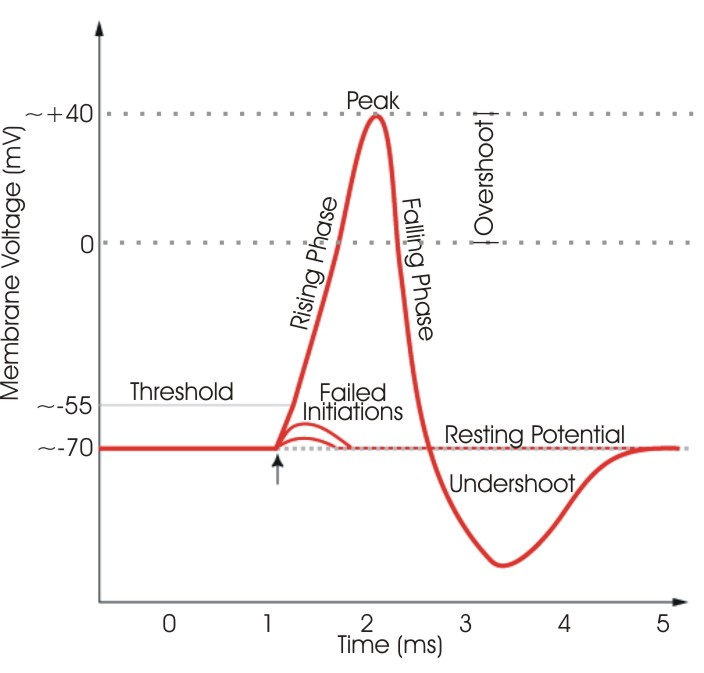
\includegraphics[width=0.7\linewidth]{../images/biosignals/action_potential.jpg}
    \captionsetup{width=0.6\linewidth}
    \captionsetup{justification=centering}
    \caption{Chart of the membrane potential during the action potential process in a neuron. Figure from Synaptidude, GFDL 1.2, via Wikimedia Commons.} 
    \label{fig:biomedical_signals_action_potential}
\end{figure}



% | | | | | | | | | | | | |

\subsubsection{EEG measures postsynaptic potentials}
\label{subsubsec:biomedical_signals_biosignals_in_human_how_postsynaptic_potential}

Whilst the action potential explains how most changes in membrane potential of an individual neuron occur, it is highly unlikely to be measured by \gls{eeg} and other measuring modalities.
This follows from the fact that, as discussed earlier, many billion neurons make up the brain making it impossible to monitor a singular neuron.
Since action potentials are such rapid current flows, it is highly unlikely enough neighbouring neurons will have an action potential at the same time resulting in a measurable signal.
However, whilst it was discussed how neurotransmitters can cause depolarization which can initialize action potentials, these neurotransmitters can also influence the membrane potential in the opposite direction by causing further polarization.
The release of these neurotransmitters and the binding to the receiving neuron also causes currents known as postsynaptic potentials.
Whilst these are not action potentials, they are essentially what causes an action potential to take place and the action potential can also cause the release of neurotransmitters.
These postsynaptic potentials are present for a longer period than action potentials.
Thus, it is more likely for many neighbouring neurons to have active postsynaptic potentials simultaneously.
The summation of these postsynaptic potential currents from many millions of neurons is what is detected by \gls{eeg}.
However, neurons experiencing action potential at that same time are among many other things sources of noise in this summation of these currents.


% - - - - - - - - - -
% why produced
% - - - - - - - - - -

\subsection{The function of bioelectricity in the human body}
\label{subsec:biomedical_signals_biosignals_in_human_why}

% TODO: start here, short section

% Complete this further but with link to previous on how it is produced

Bioelectricity is omnipresent in the human body. 
The human nervous system relies on bioelectricity to quickly carry \textit{messages} from the human body to the brain and the other way around.
The process of muscle contraction is started when action potentials, which are tiny bursts of bioelectricity, from motor neurons are transmitted to muscle fibres.
\Citet{bioelectricity_baby} explains how bioelectricity even plays a crucial role in developmental biology.
As discussed by \citet{bioelectricity_cancer}, bioelectricity can even be \textit{hijacked} as a way of novel medicine and treatment, i.e. for cancer treatment.
Listing all of the uses for bioelectricity falls outside the scope of this master thesis but it should be apparent that bioelectricity is one of the more vital phenomena in the human body.

% ---------------------------------------------- 
% BIOSIGNALS FROM THE BRAIN
% ---------------------------------------------- 

% TODO 'bci paradigms" 
% info about signals: https://www.e-iji.net/dosyalar/iji_2021_2_48.pdf

\section{Biosignals in the human brain}
\label{sec:biomedical_signals_from_brain}

% \gls{elecbiosignal}
\lipsum[1-2]


% - - - - - - - - - -
% anatomy
% - - - - - - - - - -

\subsection{Anatomy of the brain}
\label{subsec:biomedical_signals_from_brain_anatomy}

% al getoond in bci chapter

\lipsum[1-2]

% - - - - - - - - - -
% Brain waves
% - - - - - - - - - -

\subsection{Brain waves}
\label{subsec:biomedical_signals_from_brain_brain_waves}
% table wolf

\lipsum[1-3]

% - - - - - - - - - -
% Measurable brain activity
% - - - - - - - - - -

\subsection{Common brain signal inducing methods}
\label{subsec:biomedical_signals_from_brain_inducing_methods}

% bci_applications heeft ook overview onder 6. BCI electrical signa

% TODO
% echt uitleggen wat ERP is
% ssvep
% p300 zeker
% MI
% erd

\lipsum[1-7]

% TODO zie chapter 23 bci_handbook
% Issues MI: https://www.frontiersin.org/articles/10.3389/fnins.2021.824759/full
\Gls{mi} is the process in which a person generates brain-activity in the motor cortex merely by imagining motor movements.
\Gls{mi}-based \glspl{bci} are interesting because they don't require any external stimulus nor effective motor movements

\glspl{erp} and the measurable signals they produce, such as the P300 signal, are only one of many sources for detectable brain signals.
In general, \gls{erp} related signals are easier to detect reliably, as the stimulus can be controlled, giving a hint when and where to look for signals and what to look for.

An alternative to \glspl{erp} is using a mental phenomenon called \gls{mi} as source of signals for a \gls{bci} system.
\Gls{mi} is the process in which a person generates brain activity in the motor cortex merely by imagining motor movements.
Section \ref{subsec:biomedical_signals_from_brain_inducing_methods} explains in further detail how \gls{mi} is not dependent on an external stimuli nor actual motor movements.
This makes \gls{mi}-based \glspl{bci} extra appealing as they don't require external stimuli and are applicable for people with motor disabilities.
\Citet{first_mi} were the first to experiment with the idea of using \gls{mi} in an \gls{eeg} classification task.
Since then, many \gls{mi}-based \glspl{bci} have been proposed.
% MI can be trained

% - - - - - - - - - -
% generalisation issues
% - - - - - - - - - -

\subsection{Generalisation issues of brain activity}
\label{subsec:biomedical_signals_from_brain_generalisation}

% neuroplasticity and inter-human variation en non stationarity en mapping brain en... bespreken


\lipsum[1-3]

% ---------------------------------------------- 
% MEASURING BRAIN SIGNALS
% ---------------------------------------------- 

\section{Measuring brain-signals}
\label{sec:biomedical_signals_measuring}

\lipsum[1-2]

% TODO: Different affordable consumer-grade EEG devices have appeared in both Academia (e.g. [5, 6, 7, 8]) and the market (e.g. B-Alert X10, NeuroSky, OpenBCI, Emotiv)
% FROM: cheap_bci_feasibility

% ook zeker herhalen spatial resolution en dat we niet 1 neuron measuren en nooit dat zullen kunnen wss


% There is a wide variety in the devices used for the acquisition of each signal. For EEG, the number of recorded channels (electrodes) varies from a single channel to 64 channels, with sampling frequencies ranging from 128 to 1000 Hz. For the types of electrodes used, there is no dominating type with both wet and dry, and active and passive electrodes being
% hybrid bci bespreken als zijnde combinen sttrenghts: One example of such a hybrid system is to combine EEG and EMG for movement detection (Leeb et al 2011, Loopez-Larraz et al 2018, Tortora et al 2020b), as this allows detection
% uit bci_review_arnau

Many comparisons between different types of measuring equipment, often with greatly differing costs, have already been made \citep{bci_cheap_viability1, bci_cheap_viability2, bci_cheap_viability3, bci_cheap_viability4, bci_cheap_viability5}.
The main consensus is that the cheaper consumer-grade equipment has the potential to reach similar performance of a conventional, often medical-grade, BCI system.
These results are promising but due to the controlled nature of the experiments, they might not reflect real-life applications accurately.
As discussed before, the user experience of a \gls{bci} system is as important if not more important then the raw performance of the system.
% FROM: cheap_bci_feasibility
% OpenBCI1 is an open-source, versatile and affordable biosensing system which can be used to acquire not only EEG signals but also to measure electrical activity of muscle (EMG) and heart (ECG). All OpenBCI boards are based on the open-source electronic platform Arduino with wireless connection to the computer. OpenBCI offers a variety of low-cost amplifiers (boards), electrode systems (e.g. 3D-printed headware) and a software for viewing and recording the biosignals (OpenBCI GUI).2
% as well as from the user’s comfort perspective [4, 13, 14].

% - - - - - - - - - -
% Measuring modalities
% - - - - - - - - - -

\subsection{Measuring modalities}
\label{subsec:biomedical_signals_measuring_modalities}
% EEG ECOG ETC ETC

% Ook inviasive bespreken en wat het is 

% kijk naar wolf ook voor welke types

% bci_applications heeft ook overview onder 5. Signal acquisition

% Several types of EEG paradigms can be distinguished and are discussed in more detail in other reviews of Ramadan and Vasilakos (2017) and Rashid et al (2020).

% ecog: Modalities include the electrocorticogram where electrodes are implanted on the top of the cortex, right under the skull. There is also the possibility to implant electrodes directly in the brain matter (intracortical EEG) to further increase SNR and spatial resolution. However, such invasive approaches fall outside of the scope of this article.

% Alternative signals include magnetoencephalogram (Gross 2019), functional near infrared spectroscopy (Naseer and Hong 2015), and functional Magnetic Resonance Imaging (Sitaram et al 2007). Lesser known signal types are also becoming usable, such as acoustic resonance (Norman et al 2021), which uses the Doppler effect to detect changes in brain activity, and Photoplethysmogram (Han et al 2020), which uses optical reflections to monitor brain activity, in a similar way to near infrared spectroscopy. Another possibility is to monitor spinal cord activity using magnetospinography (Sakakiet al 2020) if one is only interested in lower-limb activity
% UIT bci_review_arnau

% TODO
\lipsum[1-7]

Research by \citet{human_eeg_discovery} is the first in describing the measurement of brain waves from the human skull in a non-invasive manner.
Because of this, the German neuroscientist and psychiatrist Hans Berger is often seen as the inventor of \gls{eeg}.
Whilst he was one of the first to use the term \textit{elektrenkephalogramm}, it was Richard Caton who first described the findings of brain waves in general.
He found this phenomena in animal brains as early as 1875 \citep{first_eeg}.
Since then, \gls{eeg} methodology and equipment has matured and evolved a lot.

% - - - - - - - - - -
% EEG standards
% - - - - - - - - - -

\subsection{Standards for EEG measuring systems}
\label{subsec:biomedical_signals_measuring_standards}

% TODO
\lipsum[1-2]

% - - - - - - - - - -
% available equipment
% - - - - - - - - - -

\subsection{Comparison of available EEG measuring equipment}
\label{subsec:biomedical_signals_measuring_equipment}

% TODO
todo
\lipsum[1-7]

% https://imotions.com/blog/eeg-headset-prices/
% Nextmind 
% Neurosky
% Interaxon
% Muse
% Emotiv
% myBrain
% OpenBCI
% Emotiv EPOC headset

% TODO: citing for sources of img?
% this image was here: https://docs.google.com/document/d/1uaRHNNBJsR8vqT50TllE8s3Jf2dUtAVCcLJb-vhncMM/edit

% - - - - - - - - - -
% artefacts
% - - - - - - - - - -

\subsection{Common EEG artefacts}
\label{subsec:biomedical_signals_measuring_artefacts}

% TODO also discuss how to use them e.g. eye blink as input, ook bespreken niet goed voor e.g. sroke patienten
\lipsum[1-5]

% ---------------------------------------------- 
% CONCLUSIONS OF CHAPTER
% ---------------------------------------------- 
\section{Motivation for using non-invasive MI EEG and chapter conclusions}
\label{sec:biomedical_signals_eeg_motivation_and_summary}
% TODO: summary of this chapter

% uitleggen waarom EEG en MI

\lipsum[1-3]
% TODO:
%   - Kijk na of titels in header overflowen
% ----------  
% Questions:
%   - XXX


% In a new chapter, reset the GLS to once again use full version in first occurence
\glsresetall

\chapter{Decoding brain signals with machine learning}
\label{ch:processing_signals}

% ---------------------------------------------- 
% INTRODUCTION
% ---------------------------------------------- 
\section{Introduction to this chapter}
\label{sec:processing_signals_introduction}
% NOTE: "Introduction" exists in each chapter and gives short intro to chapter + what can be expected in chapter

The previous chapter, Chapter \ref{ch:biomedical_signals} discussed \gls{biosignal} and how bioelectricity is made in the human body.
Multiple modalities for measuring brain signals were discussed and it was discussed how \gls{eeg} seems like the most promising measuring modality for capturing \gls{elecbiosignal} from the brain in a \gls{bci} setting.
Chapter \ref{ch:biomedical_signals} also discussed that \gls{mi} is one of many methods to induce such \gls{elecbiosignal} activity in the brain, namely by causing \gls{ers} and \gls{erd}.
\gls{mi} and \gls{ers}/\gls{erd} were deemed interesting as it doesn't require the external stimuli that \gls{ep} do and applies to many people, even those with limited mobility.
However, it was also discussed that \gls{ers}/\gls{erd} following from methods such as \gls{mi} require extensive user training and are harder to detect than most \gls{ep} alternatives for inducing such \gls{elecbiosignal} activity in the brain.

This chapter will discuss how brain signals can be decoded using both traditional two-step \gls{ml} and one-step \gls{dl} in a supervised manner.
Whilst Chapter \ref{ch:bci} already highlighted multiple breakthroughs in this regard on an intuitive level, this chapter will provide more technical details.
First, the general pipeline for classifying brain signals and \gls{mi} \gls{eeg} in particular is discussed.
Then the role of \gls{ml} and \gls{dl} in this pipeline and some of the most important concepts from these technologies are discussed.
This chapter then goes over the process of evaluating and using the created and trained pipelines.
The chapter concludes by discussing some of the common issues encountered while creating these pipelines and the conclusions that can be made from this chapter.


% ---------------------------------------------- 
% GENERAL TRAINING PIPELINE
% ---------------------------------------------- 
\section{A general pipeline for classifying brain signals}
\label{sec:processing_signals_general_pipeline}

\begin{sidewaysfigure}
    \centering
    \begin{subfigure}{\textwidth}
        \centering
        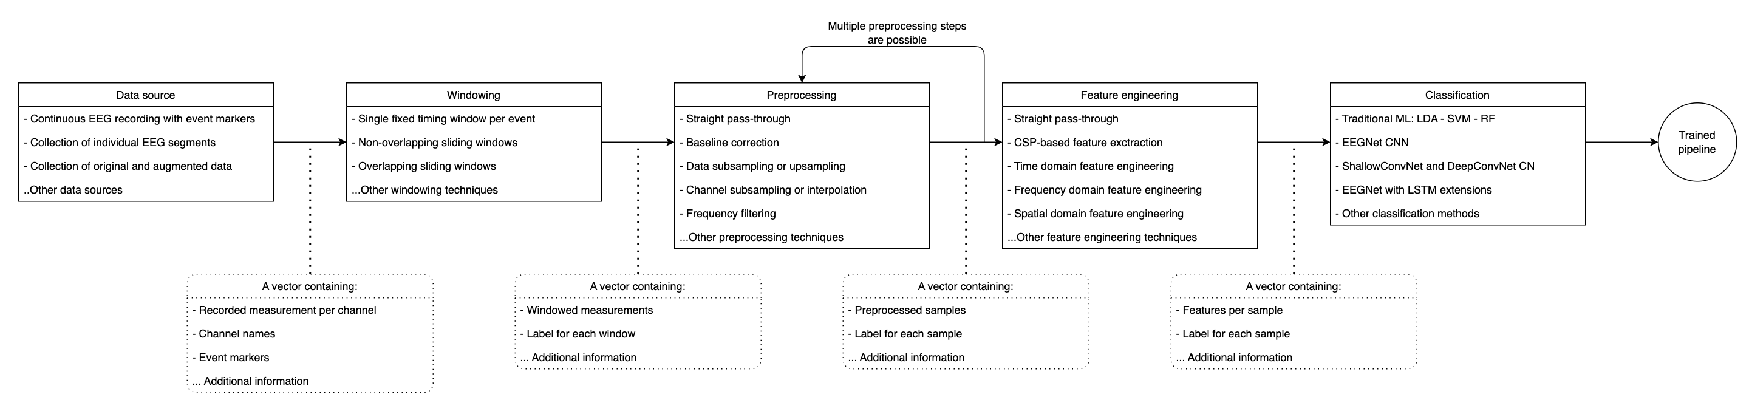
\includegraphics[width=\textwidth]{../images/pipeline/brain_signal_pipeline_training.pdf}
        \captionsetup{width=0.9\linewidth}
        \captionsetup{justification=centering}
        \caption{Components of general training pipeline for brain signal classification annotated with common examples per component.}
        \label{fig:processing_signals_pipeline_ml}
    \end{subfigure}
    \hfill
    \begin{subfigure}{\textwidth}
        \centering
        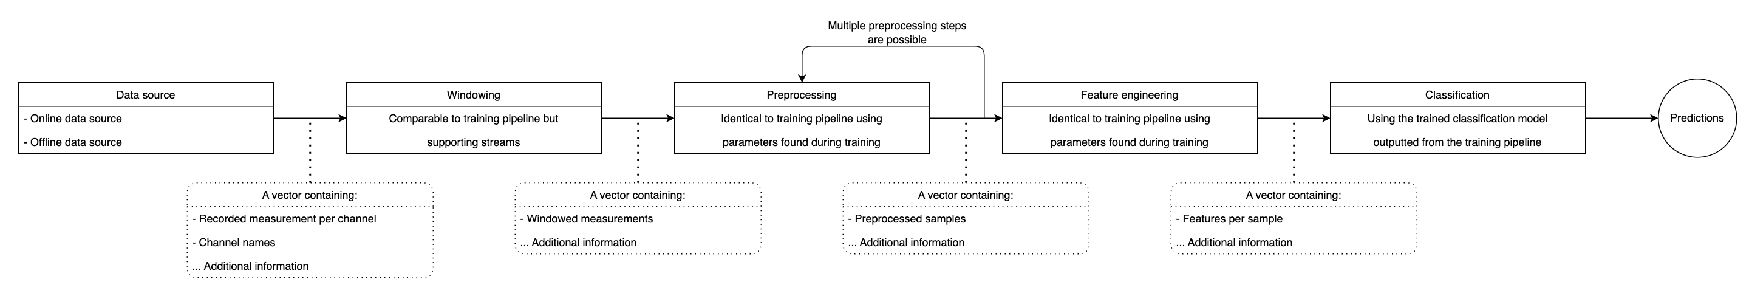
\includegraphics[width=\textwidth]{../images/pipeline/brain_signal_pipeline_predicting.pdf}
        \captionsetup{width=0.9\linewidth}
        \captionsetup{justification=centering}
        \caption{Components of general prediction pipeline for brain signal classification annotated with common examples per component.}
        \label{fig:processing_signals_pipeline_dl}
    \end{subfigure}
    \captionsetup{width=0.9\linewidth}
    \captionsetup{justification=centering}
    \caption{General training pipeline and prediction pipeline used for classifying brain signals.}
    \label{fig:processing_signals_pipeline}
\end{sidewaysfigure}

The general pipeline of classifying brain signals and \gls{eeg}-based \gls{mi} tasks in particular is similar to that of a \gls{cad} systems which was discussed in Section \ref{subsubsec:bci_gaining_popularity_improved_data_processing_better_ml_dl} and shown in Figure \ref{fig:cad_pipeline}.
Whilst the training pipeline and prediction pipeline for classifying brain signals consist of the same components, their input and output are different.
For this reason, this master thesis considers them as two separate pipelines.
The remainder of this section will discuss the components used in these brain signal classification pipelines and the techniques commonly used in each of these components.
Figure \ref{fig:processing_signals_pipeline} provides a visual overview of these pipelines and their components.

% - - - - - - - - - -
% Data acquisition
% - - - - - - - - - -

\subsection{Data source}
\label{subsec:processing_signals_general_pipeline_data_acquisition}

Assuming supervised learning, a \gls{ml} paradigm further discussed in Section \ref{subsec:processing_signals_ml_and_dl_tyes_of_learning_supervision}, input data for the training pipelines should include both the independent variables as wel the dependent variable.
When working with an \gls{eeg} \gls{mi} classification problem, these independent variables are the \gls{eeg} measurements of each channel whilst the dependent variable is the \gls{mi} task performed at a specific time point.
Multiple possibilities exist for providing these variables and the link between them.
Most open-source \gls{mi} \gls{eeg} datasets, such as the one by \citet{eeg_data} used in this master thesis, do this by providing the \gls{eeg} recordings of an entire session as a single 2D matrix (channels x measurement per time point) and the desired labels as an equal width vector containing the marker at any given time point.
The time points are dependent on the sampling frequency and denote the sample number counting from the first sample of the session.
The marker may be the current content of the screen which provides tasks to the user or other event-related information.
Figure \ref{fig:processing_signals_data_source_eeg} combines both the independent and dependent variables into a singular visualisation.

The prediction pipeline only expects the independent variables as its task is to predict the dependent variable.
In theory, these independent variables should be of the same format used during training, but in practice, they might originate from a different source or recording and as such might require additional steps during preprocessing to ensure at least an equal sampling frequency and channel distribution.
This master thesis assumes the device used during training and prediction is identical with equal settings used and as such doesn't require this type of preprocessing.

The prediction pipeline may work in an offline manner, as is the case for the experiments in this master thesis, or in an online manner.
When using offline prediction the data was already recorded and stored before being provided in its totality to the prediction pipeline.
In an online setting, the data is streamed to the prediction pipeline as it is being measured and the prediction pipeline should merge this incoming data to an object that is usable in the next stages itself.
For example, a buffer may be used to collect samples until one second is obtained and pass that to the next step.
In an online setting, windowing is often directly performed on the stream, as discussed next.
Other types of data formatting are possible but they should all provide the same information.

\begin{figure}[ht]
    \centering
    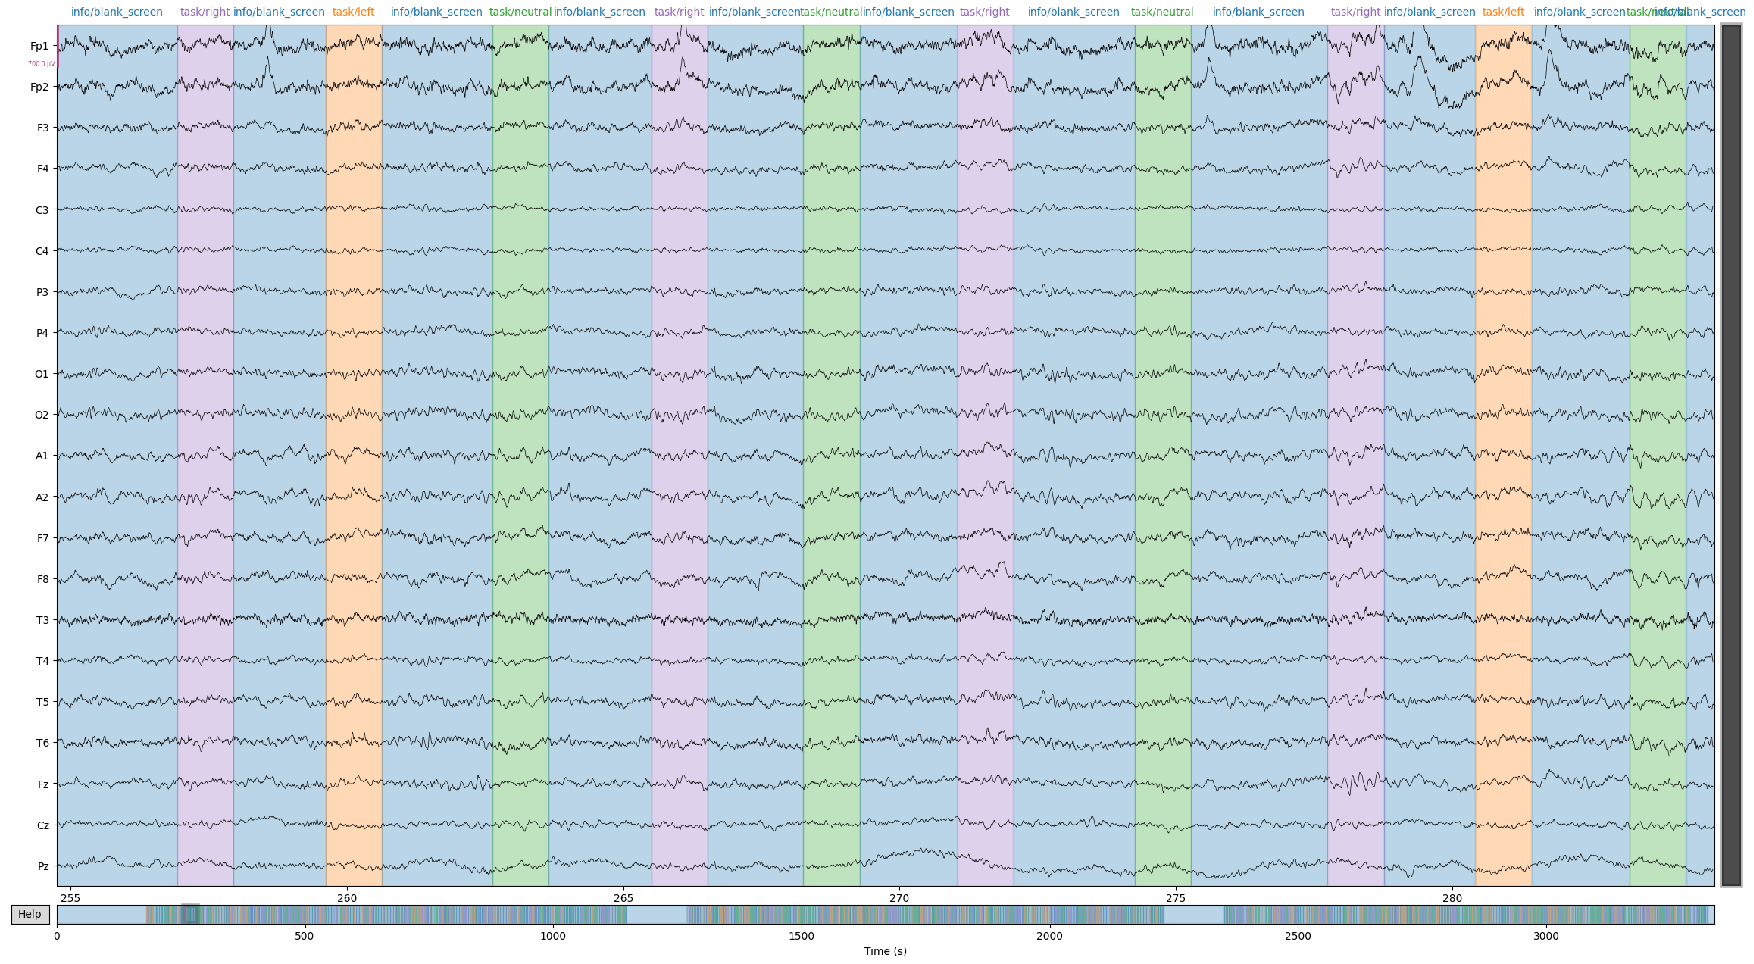
\includegraphics[width=\linewidth]{../images/pipeline/eeg.pdf}
    \captionsetup{width=0.9\linewidth}
    \captionsetup{justification=centering}
    \caption{Visualisation of the \gls{eeg} recording from December 15 2015 overlayed with the provided markers for subject B in the open-source dataset by \citet{eeg_data}. The x-axis depicts the time in seconds, the y-axis depicts which channel of the recording is visualised and the colour overlay represents the active marker.}
    \label{fig:processing_signals_data_source_eeg}
\end{figure}

% - - - - - - - - - -
% Windowing
% - - - - - - - - - -

\subsection{Windowing}
\label{subsec:processing_signals_general_pipeline_windowing}

The data source as described in Section \ref{subsec:processing_signals_general_pipeline_data_acquisition} provides a continous signal over multiple channels.
To process these signals a mechanism has to be in place so that this continuous signal is split into discrete segments.
Such techniques are often referred to as windowing, but the neurophysiological field also refers to it as epoching.
The latter should not be confused with the meaning of epochs in a \gls{ml} setting.
Different types of windowing exist and three common approaches are illustrated in Figure \ref{fig:processing_signals_windowing}.
Using a fixed window surrounding known event points is trivial on the training data and results in the simplest classification task with the most consistent window labels from the three windowing techniques shown in Figure \ref{fig:processing_signals_windowing}.
However, when trying to predict outcomes, the point at which an event occurs has to be known as well.
This information may be known, for example during an offline \gls{mi} classification task or when using a fixed feedback loop in an online manner where actions from the user are accepted at fixed time intervals.

\begin{figure}[ht]
    \centering
    \begin{subfigure}{0.45\textwidth}
        \centering
        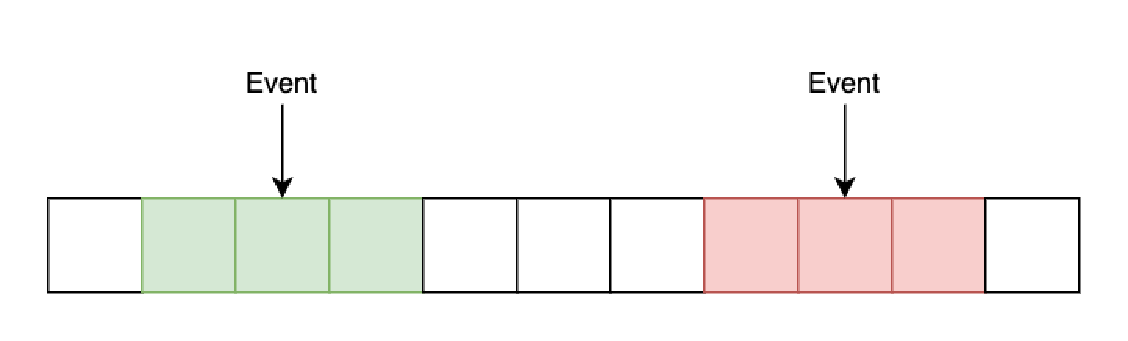
\includegraphics[width=\textwidth]{../images/pipeline/fixed_window.pdf}
        \captionsetup{width=\linewidth}
        \captionsetup{justification=centering}
        \caption{Fixed window surrounding a known event.}
        \label{fig:processing_signals_windowing_non_fixed}
    \end{subfigure}
    \hfill
    \begin{subfigure}{0.45\textwidth}
        \centering
        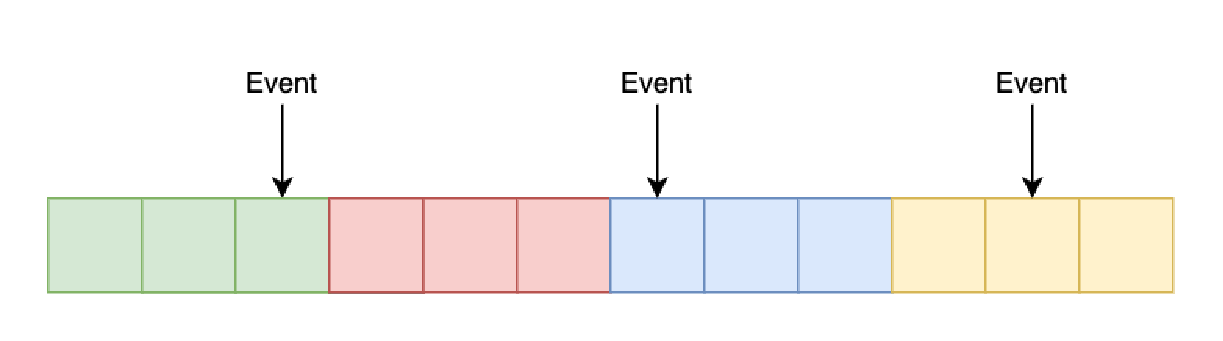
\includegraphics[width=\textwidth]{../images/pipeline/non_overlapping_window.pdf}
        \captionsetup{width=\linewidth}
        \captionsetup{justification=centering}
        \caption{Non-overlapping sliding windows.}
        \label{fig:processing_signals_windowing_non_overlapping}
    \end{subfigure}
    \hfill
    \begin{subfigure}{0.45\textwidth}
        \centering
        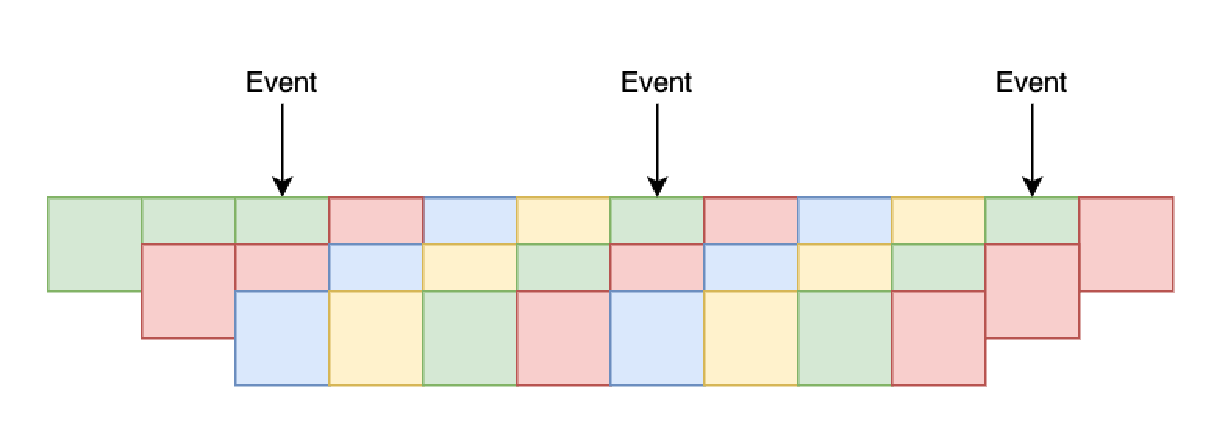
\includegraphics[width=\textwidth]{../images/pipeline/overlapping_window.pdf}
        \captionsetup{width=\linewidth}
        \captionsetup{justification=centering}
        \caption{Overlapping sliding windows}
        \label{fig:processing_signals_windowing_overlapping}
    \end{subfigure}
    \captionsetup{width=\linewidth}
    \captionsetup{justification=centering}
    \caption{Different types of windowing techniques.}
    \label{fig:processing_signals_windowing}
\end{figure}

A more intuitive but computationally harder windowing technique is using sliding windows.
A non-overlapping sliding window technique is shown in Figure \ref{fig:processing_signals_windowing_non_overlapping} and an overlapping technique is shown in Figure \ref{fig:processing_signals_windowing_overlapping}.
Both are trivial to apply to the independent variables but deciding which dependent variable should be related becomes a difficult task.
How much activity from the event should be included for the training window to be considered a sample of that event?
What happens when a window includes two distinct events?
These are questions that should be answered within the context of the application.
When using sliding windows, singular labels such as "task right" may be split into "task right start", "task right hold" and "task right end".

Many different windowing techniques exist that use far more complex strategies than the ones illustrated in Figure \ref{fig:processing_signals_windowing}, especially for controlling the boundaries of the window.
\citet{complex_windowing} discuss some of these more complex windowing techniques in more detail.
When done right, certain sliding window techniques can improve the performance of a \gls{mi} \gls{eeg} classification pipeline compared to even fixed windowing surround a known event, as shown by \citet{sliding_windows_better}.
However, starting a new sliding window at each time point may cause significant computational overhead, increasing both training and prediction time.
The latter can make the prediction pipeline too complex to be run on affordable, low-energy and portable computational hardware as desired by a \gls{bci} system doing local processing.
This master thesis will consider a fixed window of 0.5 seconds and 1.5 seconds surround a known event for both training and prediction.

% - - - - - - - - - -
% Preprocessing
% - - - - - - - - - -

\subsection{Preprocessing}
\label{subsec:processing_signals_general_pipeline_preprocessing}

Brain signals are non-linear as well as non-stationary signals and exact execution of the performed \gls{mi} tasks are bound to differ per subject as already discussed in section \ref{subsec:biomedical_signals_working_with_eeg_generalisation}.
Combining these properties with the poor \gls{snr} of \gls{eeg}, as discussed in Section \ref{tab:biomedical_signals_modalities}, means that raw \gls{eeg} measurements are hard to intepret, even by machines.
Luckily, as discussed by \citet{bci_review_arnau}, a \gls{dl} approach making use of sufficient layer, nodes and training should be capable of learning any mapping from input to output, including any manual preprocessing that can be done.
As such, \gls{dl} approaches can often work directly on this raw \gls{eeg} signal and raw signals in general.
This is one of the most promising aspects of \gls{dl} in multiple fields and it is the reason the one-step \gls{dl} approaches from this master thesis will use no preprocessing besides the \gls{ac} artefact removal that was already performed by the suppliers of the open-source database \citep{eeg_data}.
Traditional two-step \gls{ml} approaches do not have this property of being able to learn any mapping from input to output and as such require at least minimal preprocessing of the data to obtain usable results.
For this reason, many libraries providing the most basic \gls{eeg} preprocessing steps have been developed with MNE by \citet{mne} being the most popular for Python and used in this master thesis.
Some automated pipelines specifically for \gls{eeg} preprocessing have also been proposed, such as the PREP pipeline by \citet{prep_pipeline}. 

% | | | | | | | | | | | | |

\subsubsection{Frequency filtering}
\label{subsubsec:processing_signals_general_pipeline_preprocessing_filter}

One of the most common preprocessing operations done to \gls{eeg} signals is frequency filtering.
Frequency filters come in four main categories: low-pass filters, high-pass filters, band-pass filters and band-stop filters.
The working of these filters in the frequency domain is shown in Figure \ref{fig:processing_signals_filters}.
Again, many variants on how to exactly perform the filter exist.
Some use a harsh filter with no transition band whilst others use a transition band as visualised in Figure \ref{fig:processing_signals_filters}.
As further discussed by \citet{fir_iir_filter}, a first distinction is made between \gls{fir} and \gls{iir} filters.
Most common filter operations are using a band-stop filter to cancel out the \gls{ac} artefacts discussed in Section \ref{subsec:biomedical_signals_working_with_eeg_artefacts} and to filter out frequencies not of interest for the application.
Since these operations are so common they are often included directly in \gls{eeg} equipment with a hardware filter.
This master thesis uses a \gls{fir} filter design using the Blackman window method in some of its experiments to band-pass filter the signal to only include the \gls{mi} frequencies as discussed in Section \ref{subsec:biomedical_signals_working_with_eeg_brain_waves}.
Further details of this exact filter are not of interest for this master thesis and the MNE library supplied functionality is used to obtain the desired filter \citep{mne}.


\begin{figure}[t]
    \centering
    \begin{subfigure}{0.45\textwidth}
        \centering
        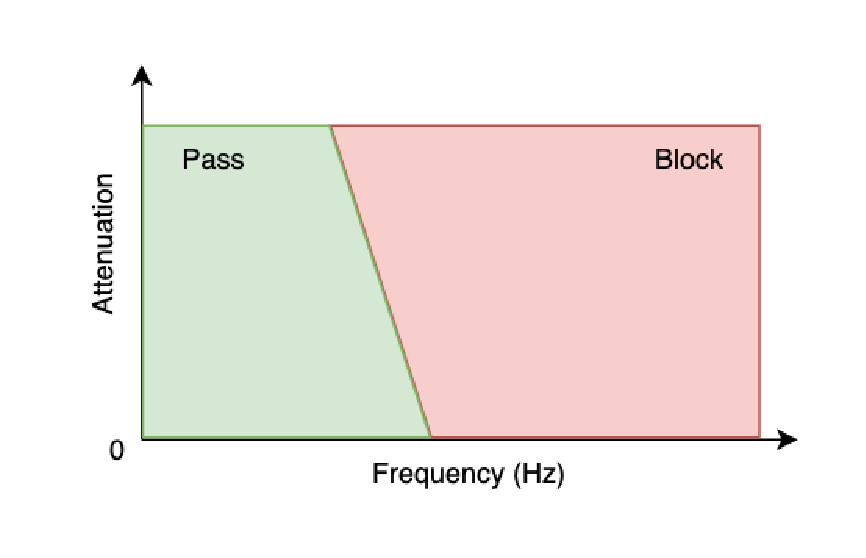
\includegraphics[width=\textwidth]{../images/pipeline/lowpass_filter.pdf}
        \captionsetup{width=\linewidth}
        \captionsetup{justification=centering}
        \caption{Low-pass filter.}
        \label{fig:processing_signals_filters_lowpass}
    \end{subfigure}
    \hfill
    \begin{subfigure}{0.45\textwidth}
        \centering
        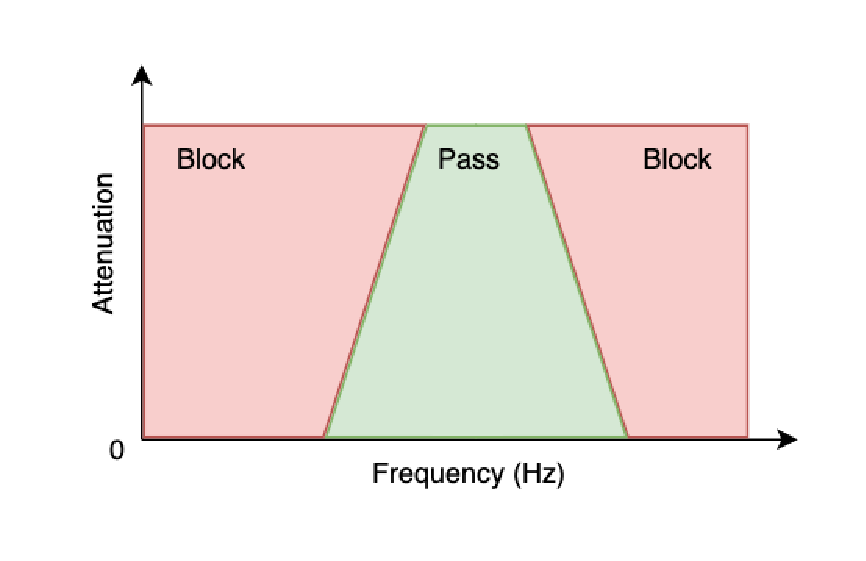
\includegraphics[width=\textwidth]{../images/pipeline/bandpass_filter.pdf}
        \captionsetup{width=\linewidth}
        \captionsetup{justification=centering}
        \caption{Band-pass filter.}
        \label{fig:processing_signals_filters_bandpass}
    \end{subfigure}
    \hfill
    \begin{subfigure}{0.45\textwidth}
        \centering
        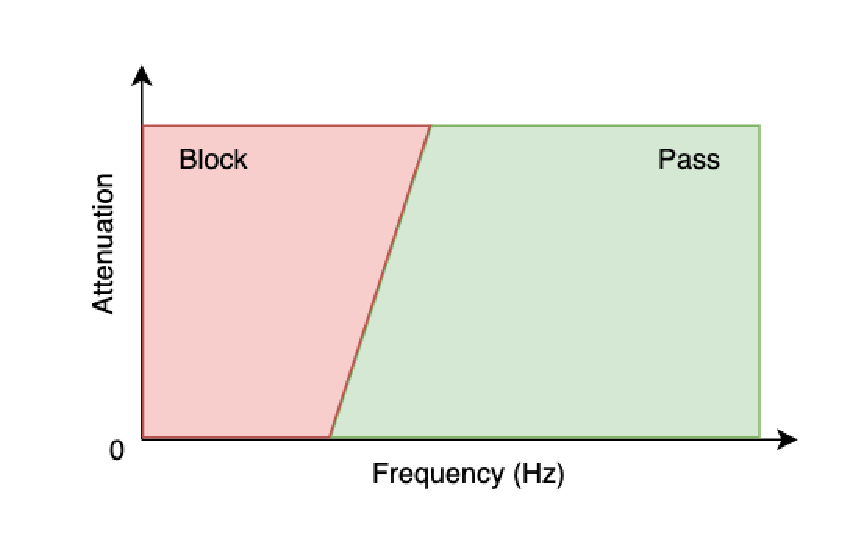
\includegraphics[width=\textwidth]{../images/pipeline/highpass_filter.pdf}
        \captionsetup{width=\linewidth}
        \captionsetup{justification=centering}
        \caption{High-pass filter.}
        \label{fig:processing_signals_filters_highpass}
    \end{subfigure}
    \hfill
    \begin{subfigure}{0.45\textwidth}
        \centering
        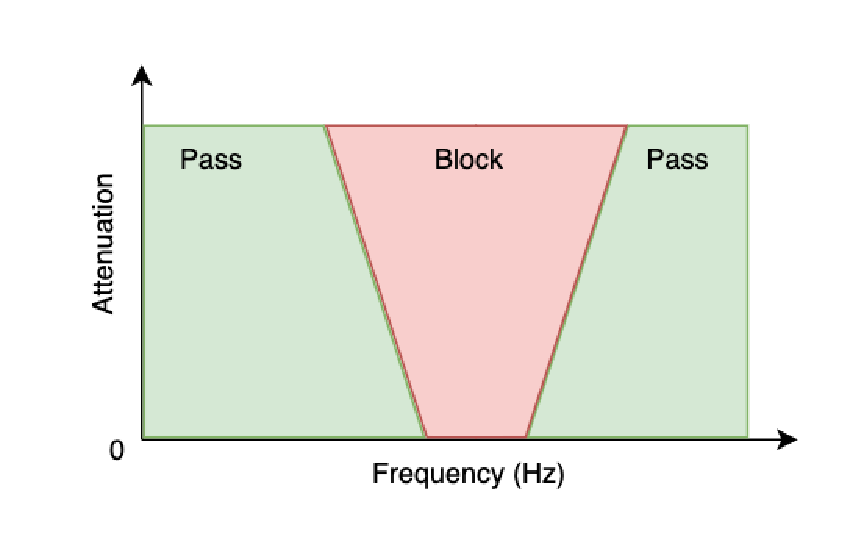
\includegraphics[width=\textwidth]{../images/pipeline/bandstop_filter.pdf}
        \captionsetup{width=\linewidth}
        \captionsetup{justification=centering}
        \caption{Band-stop filter.}
        \label{fig:processing_signals_filters_bandstop}
    \end{subfigure}
    \captionsetup{width=\linewidth}
    \captionsetup{justification=centering}
    \caption{Different types of filtering techniques.}
    \label{fig:processing_signals_filters}
\end{figure}

% | | | | | | | | | | | | |

\subsubsection{Baseline correction}
\label{subsubsec:processing_signals_general_pipeline_preprocessing_baseline_correction}

Another common preprocessing operation is baseline correction on a window.
Baseline correction consists of taking a baseline period and determining the mean voltage of each electrode's measurements during that baseline.
This baseline is most often one or more seconds before an event occurs.
This mean voltage is then subtracted from the remaining signal of each respective channel.
Doing this normalizes each window such that it has a centre closer to zero.
This can help in reducing the non-stationary problem and is used for the traditional two-step \gls{ml} experiments in this master thesis with a baseline period of one second before the event.

% | | | | | | | | | | | | |

\subsubsection{Channel and data downsampling or upsampling}
\label{subsubsec:processing_signals_general_pipeline_preprocessing_subsampling}

Another type of preprocessing is channel subsampling and augmentation through interpolation.
This consists of removing channels not of interest as discussed in Section \ref{subsec:biomedical_signals_working_with_eeg_anatomy} or adding augmented channels by clever interpolation or other approaches from the existing channels.
When a certain channel is known to be bad or artefacts described in Section \ref{subsec:biomedical_signals_working_with_eeg_artefacts} are detected, it may be replaced by an augmented channel during the artefact period as a way of resolving the artefact.
Likewise, if the sampling frequency of \gls{eeg} equipment is too high or low, data subsampling or upsampling may be performed.

% | | | | | | | | | | | | |

\subsubsection{Other preprocessing techniques and preprocessing ordering}
\label{subsubsec:processing_signals_general_pipeline_preprocessing_orders}

There exist many other preprocessing techniques for signals and \gls{mi} \gls{eeg} signals in particular but these fall outside the scope of this master thesis.
Preprocessing can happen in other places of the pipeline than the one shown in Figure \ref{fig:processing_signals_pipeline}, for example, channel subsampling reduces dimensionality and is thus often done as soon as possible to limit unneeded computational overhead.
It is important to note that multiple preprocessing steps may be performed in sequence.
This means that the output of a previous preprocessing step is used in the next and as such the ordering of preprocessing steps can be important depending on the techniques used in the sequence.
It is also important to note that certain preprocessing techniques which learn parameters from the training data should use the same parameters for the prediction pipeline, as redetermining them on the prediction data may alter the data in a way unknown by the already trained classifier later in the pipeline.
Whilst often not the case for preprocessing techniques, this is a subtility of great importance in feature engineering, the next step in the pipeline.



% - - - - - - - - - -
% Feature
% - - - - - - - - - -

\subsection{Feature engineering}
\label{subsec:processing_signals_general_pipeline_features}

Feature engineering, or feature extraction, is the process of representing raw or preprocessed data by numerical features that carry information from the original data related to the problem.
The goal of feature extraction is to simplify a complex data structure by representing it as one or many features that are easier to interpret and/or learn.
This step is crucial in traditional two-step \gls{ml} classification approaches as even the preprocessed data is often too complex for traditional \gls{ml} classifiers to directly learn from.
This differs from preprocessing which aimed to improve the raw data quality, although for some of the discussed preprocessing techniques it could be debated that they are also a type of feature extraction.
As already addressed in Section \ref{subsec:processing_signals_general_pipeline_preprocessing}, some features rely on learned parameters, such as the $\mathbf{W}$ matrix for spatial filters discussed later in this section, these learned parameters should be reused in the prediction pipeline and not redetermined on the prediction data, as this will confuse the classification model and produce unwanted behaviour.

A simple but poor feature extraction technique for \gls{eeg} data would be representing the channels' measurements not by their raw data but by their minimum, maximum, median, first quartile and third quartile, much like a boxplot would.
Whilst this would be easy to interpret, it would carry too little information for a classifier to effectively learn anything but the simplest problems.
Finding appropriate feature extraction techniques is a hard task which has taken years of refinement and has ongoing refinement in many fields, including \gls{eeg} classification and other medical imaging fields \citep{CAD_ml_dl_kbs}.
\gls{eeg} feature extraction methods can be categorized by the domain they work in, namely the time domain, frequency domain, time-frequency domain or spatial domain.
The experiments in this master thesis will only consider \gls{csp} for feature extraction in the traditional \gls{ml} classification approaches, a spatial filtering technique closely related to \gls{pca} used for mainly spatial domain feature extraction.
As discussed in Section \ref{subsec:bci_gaining_popularity_improved_data_processing}, \gls{csp} derived features are commonly used in traditional two-step \gls{ml} classification and the \gls{csp} technique has seen many extensions over the years.
\gls{csp} is further discussed together with its extensions in Section \ref{sec:offline_bci_system_two_step_ml}.

The remainder of this section briefly discusses the feature extraction possibilities in each domain but a more detailed explanation falls outside the scope of this master thesis.
The reader is reffered to chapter 7 of the \gls{bci} book by \citet{bci_book} for an in-depth overview of many feature extraction techniques for \gls{bci} applications in far greater detail.
\Citet{eeg_features} compares the performance of multiple feature extraction techniques for epileptic seizure detection using \gls{eeg}.
\Citet{time_domain_eeg_features} compares multiple feature extraction methods for \gls{eeg}-based \gls{bci} applications in the time domain whilst \citet{timefreq_domain_eeg_features} does the same for feature extraction methods in the frequency and time-frequency domain.


% | | | | | | | | | | | | |

\subsubsection{Time domain feature extraction}
\label{subsubsec:processing_signals_general_pipeline_features_timedomain}

Temporal feature extraction methods work in the time domain, where the \gls{eeg} data is analysed as a time series of voltage measurements per channel.
This is most likely the representation of the data as it comes from the previous preprocessing step in the pipeline and as such doesn't require an additional transformation.
\Citet{time_domain_eeg_features} describes some relatively simple feature extraction methods in the time domain, namely the windows's \gls{mav} per electrode, the amount of times a \gls{zc} and \gls{ssc} occurs per channel and the cumulative \gls{wl}.
When all four of these relatively simple features are combined, surprisingly good accuracies are obtained through intrasession testing \citep{time_domain_eeg_features}.

Many more time domain feature extraction techniques exist and some more examples are given by \citet{eeg_features}.
\citet{eeg_features} discusses some other simple features, including those used by \citet{time_domain_eeg_features}.
For example, the \gls{wl} feature described by \citet{time_domain_eeg_features} is called \textit{total line length} by \citet{eeg_features} and provided in Equation \ref{eq:processing_signals_line_length}.
\Citet{eeg_features} also details more complex features based on the entropy of the signal such as \gls{pe}, \gls{apen}, \gls{fuzzen} and more.

\begin{equation}
    \label{eq:processing_signals_line_length}
    L(X) = \sum_{i=1}^{N-1} |X[i] - X[i - 1]|
\end{equation}


% | | | | | | | | | | | | |

\subsubsection{Frequency domain feature extraction}
\label{subsubsec:processing_signals_general_pipeline_features_freqdomain}

As the name suggests, frequency domain feature extraction happens in the frequency domain.
The frequency domain represents the measured \gls{eeg} signals in terms of frequency rather than time as was the case for the time domain.
To extract features in the frequency domain, the signal represented in the time domain must first be transformed to its frequency domain representation.
The most common way of going from the time domain to the frequency domain is through the use of a \gls{ft} \citep{fourier_transform}.
A  \gls{ft} has the nice property that it can be converted back to the time domain by using the \gls{ift}.
The theoretical \gls{ft} and \gls{ift} make use of integrals from $-\inf$ to $\inf$ and as such can't be directly used on real data.
Many methods have been proposed to estimate this full integral solution, with the \gls{dft} and \gls{idft} being the most common.
The \gls{dft} and \gls{idft} equations are given in Equation \ref{eq:processing_signals_dft} and \ref{eq:processing_signals_idft} respectively.
The output of the \gls{dft} ($X_k$) is a complex number that represents the amplitude and phase of a sinusoidal wave, representing the signal in the frequency domain.
The frequency of this sinusoidal wave is $\frac{k}{N}$ derived from Euler's formula.
\Citet{fast_fourier_explained} discusses the \gls{ft}, \gls{ift}, \gls{dft} and \gls{idft} in more detail.
\Citet{fast_fourier_explained} also discusses that the computation of \gls{dft} can be too complex for many applications and introduces the \gls{fft}, a faster variant of \gls{dft}.
\Gls{fft} is the algorithm that is most commonly used for effective conversion between the time and frequency domain in computer applications.

\begin{equation}
    \label{eq:processing_signals_dft}
    X_k = \sum_{n=O}^{N-1} x_n e^{\frac{-2 \pi i k n}{N}}
\end{equation}

\begin{equation}
    \label{eq:processing_signals_idft}
    x_n = \frac{1}{N} \sum_{k=O}^{N-1} X_k e^{\frac{2 \pi i k n}{N}}
\end{equation}

Once the signal is represented in the frequency domain, most of the frequency domain features are extracted from the \gls{psd}.
The \gls{psd} is a visualisation of the power levels of the frequency component present in the signal.
Figure \ref{fig:processing_signals_psd} show the \gls{psd} of the \gls{eeg} signals previously shown in  Figure \ref{fig:processing_signals_data_source_eeg}.
Note the sharp trough present at 50\gls{hz} due to the \gls{ac} artefact removal that is done by a band-stop filter at that frequency.
As discussed further by \citet{eeg_features}, the features extracted from the \gls{psd} include the energy, \gls{iwmf} and \gls{iwbw} among others.

\begin{figure}[t]
    \centering
    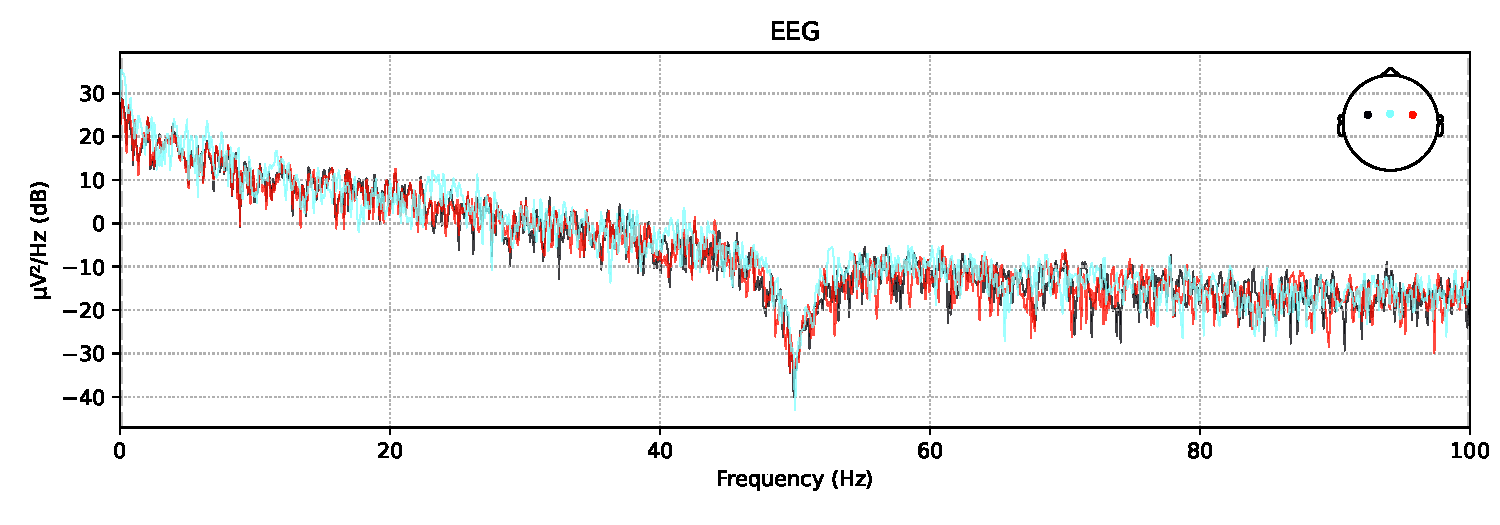
\includegraphics[width=\linewidth]{../images/pipeline/psd.pdf}
    \captionsetup{width=0.9\linewidth}
    \captionsetup{justification=centering}
    \caption{\Glsfirst{psd} for the \gls{eeg} signal previously shown in Figure \ref{fig:processing_signals_data_source_eeg}. Only the C3, Cz and C4 channels are shown.}
    \label{fig:processing_signals_psd}
\end{figure}

% | | | | | | | | | | | | |

\subsubsection{Time-frequency domain feature extraction}
\label{subsubsec:processing_signals_general_pipeline_features_timefreqdomain}

Whilst it is possible to extract features from both the time and frequency domain and rely on the classifier to learn a mapping between them, attempts have been made at combining both domains.
For example, when further windowing the time domain signal into short time segments and using a \gls{ft} on those shorter time segments, a \gls{stft} is obtained.
\Gls{stft} assumes that those shorter time segments are stationary, even if the complete signal from which those time segments are taken was non-stationary.
This allows for using frequency-domain feature extraction on those shorter \gls{ft} signals.
This will result in features that represent frequency domain characteristics but are ordered in a time respective order.
These features could then be seen as individual data points in the time domain and thus can be further processed with time-domain feature extraction techniques.

However, the use of \gls{stft} in \gls{eeg} applications is limited as finding a balance between long enough time segments such that the \gls{ft} is meaningful but short enough so that enough time domain information is retained has been proven challenging.
A better alternative is using \gls{wt}, a technique that has been proven powerful in image compression and many other fields \citep{wavelet_transform_uses}.
Compared to the \gls{ft} that works with sinusoidal waves, \gls{wt} works with wavelets.
These wavelets are characterised by their scale and location.
The scale relates to the frequency domain whilst the location relates to the time domain, showing a clear link with the time-frequency domain.
Compared to \gls{stft}, \gls{wt} does not make any assumptions about stationarity.
The book by \citet{book_wavelet} discusses \gls{wt} in detail.
The technical details and related feature extraction methods of which fall outside the scope of this master thesis.

% | | | | | | | | | | | | |

\subsubsection{Spatial domain feature extraction}
\label{subsubsec:processing_signals_general_pipeline_features_spatialdomain}

As discussed in Section \ref{subsec:biomedical_signals_measuring_brain_modalities}, \gls{eeg} has a relatively poor spatial resolution.
This would suggest that feature extraction based on the spatial domain is bound to perform poorly as well, bet this is not the case.
Many \gls{bci} systems rely on features extracted from \gls{eeg} signals that were spatially filtered with techniques such as \gls{pca}, \gls{ica} and \gls{csp} \citep{bci_book}.
To understand spatial filters, it should be repeated that \gls{eeg} channels don't represent the value of a singular electrode but rather the output of applying a differential amplifier on two channels, as was discussed in Section \ref{subsec:biomedical_signals_measuring_brain_modalities}.
If all these channels have one electrode in common, an alternative set of channels can be created by weighing and combining the original channels \citep{bci_book}.
This is the main idea behind spatial filtering and can be mathematically represented as the matrix equation shown in Equation \ref{eq:processing_signals_spatial_filter}.
In this equation, $\mathbf{X}$ represents the 2D matrix of $N$ channels and $P$ samples.
$\mathbf{W}$ represents the weight matrix with $M$ spatial filters and $N$ channel weights.
Finally, $\mathbf{Y}$ represents the alternative set of channels with $M$ spatially filtered channels and $P$ samples.

There are both data-independent and data-dependent techniques for determining the weight matrix $\mathbf{W}$ of Equation \ref{eq:processing_signals_spatial_filter}.
In some regards, the average reference montage shown in Figure \ref{fig:biomedical_signals_eeg_montages} can be considered a data-independent spatial filter, as it uses a fixed, data-independent $\mathbf{W}$ matrix, namely one that averages all channels.
A more complex but comparable data-independent spatial filter is using one of many variants of surface Laplacian spatial filtering.
Intuitively, these types of Laplacian filters use only the electrodes at a certain spatial distance for determining the average.
Simple variants may consider each electrode in the region of interest equally important whilst others might use a weighted average based on the spatial distance of the electrode.
Surface Laplacian spatial filtering has proven successful in improving the source localisation capabilities of \gls{eeg} by filtering out the signals present in multiple electrodes and keeping only those unique to the electrode of interest \citep{improve_eeg_spatial_laplacian1, improve_eeg_spatial_laplacian2, improve_eeg_spatial_laplacian3}.


\begin{equation}
    \label{eq:processing_signals_spatial_filter}
    \begin{bmatrix} 
        y_{11} & y_{12} & \dots \\
        \vdots & \ddots & \\
        y_{M1} &        & y_{MP} 
    \end{bmatrix} = 
    \begin{bmatrix} 
        w_{11} & w_{12} & \dots \\
        \vdots & \ddots & \\
        w_{M1} &        & w_{MN} 
    \end{bmatrix}
    \begin{bmatrix} 
        x_{11} & x_{12} & \dots \\
        \vdots & \ddots & \\
        x_{N1} &        & x_{NP} 
    \end{bmatrix}
\end{equation}


However, by far the most commonly used spatial domain feature extraction happens on data after a data-dependent spatial filter such as \gls{pca}, \gls{ica} or \gls{csp} has been applied.
These data-dependent spatial filters optimize the $\mathbf{W}$ matrix from Equation \ref{eq:processing_signals_spatial_filter} based on measured \gls{eeg} signals.
\Gls{pca} creates a $\mathbf{W}$ matrix such that the resulting signal has the highest proportion of amplitude variance from the original signals matrix $\mathbf{X}$ \citep{bci_book}.
Whilst this can be successful, \gls{pca} only uses the values from the independent variables for creating the $\mathbf{W}$ matrix and as such the created matrix is not optimized for best discrimination of the dependent variable.
Imagine for example a $\mathbf{X}$ matrix that was not preprocessed to remove the \gls{ac} artefacts described in Section \ref{subsec:biomedical_signals_working_with_eeg_artefacts}.
Since this line current noise is so present, \gls{pca} will consider it as one of the most important \gls{pca} components even though it carries no information for the problem.
\Gls{ica} could be seen as a variant of \gls{pca} that wishes to create a $\mathbf{W}$ matrix such that the resulting signal consists of independent channels.
However, as described by \citet{bci_book}, using \gls{ica} forms multiple challenges in \gls{bci} applications due to its computational cost and often imperative way of determining the number of independent channels to be found.
Besides this, \gls{ica} also only rely on the independent variable and as such is not further considered for this master thesis.

\Gls{csp} is a type of spatial filtering closely related to \gls{pca} that does use the dependent variable to create a set of new channels that are optimized to solve the problem.
This makes \gls{csp} incredibly powerful and studied in \gls{bci} research, as already addressed in Section \ref{subsec:bci_gaining_popularity_improved_data_processing}.
\Gls{csp} will be discussed in further detail together with its extensions in Section \ref{sec:offline_bci_system_two_step_ml}.
\Citet{bci_book} provides a more in-depth overview of all three of these spatial filtering techniques.

% | | | | | | | | | | | | |

\subsubsection{The promise and downfall of feature extraction}
\label{subsubsec:processing_signals_general_pipeline_features_dl_link}

Manual feature extraction is done in what this master thesis refers to as traditional two-step \gls{ml}. 
These traditional two-step \gls{ml} approaches have some attractive properties but also some fundamental limitations.
Manual feature extraction such as the one discussed in this section mostly tries to implement human knowledge about a problem as an algorithm.
Features that are derived are those that an expert deems fit for describing and learning the problem.
This is great in terms of explainability and interpretability, as combined with the right \gls{ml} classification algorithm such as \gls{rf} it can give direct insight into how a prediction pipeline came to its conclusion.
This is desired in many fields, especially the medical one.
As described in Section \ref{subsec:processing_signals_common_issues_exaplainable}, explainability and interpretability could even become a requirement of general \gls{ai} applications.
As such, traditional two-step \gls{ml} still has significant ongoing research as is shown by the many alternatives on \gls{csp} that have been proposed, as further discussed in Section \ref{sec:offline_bci_system_two_step_ml}.

However, as discussed by \citet{CAD_ml_dl_kbs} for medical lung imaging applications, \gls{dl} that learns some form of features from data in an automated manner outperform traditional two-step \gls{ml} classification in many tasks.
This lies in the power of \gls{dl} being able to learn features that might be unknown by experts and thus can't be encoded for manual feature extraction.
Research in disease detection, such as \citet{attia} findings of using a \gls{cnn} to detect \gls{af} from normal sinus rhythm \gls{ecg} has shown just that.
Given the human understanding of the brain is still limited as discussed in Section \ref{subsec:bci_opportunities_obstacles_complex}, it is likely that the right \gls{dl} models will learn features that are far more descriptive of the problem but not yet understood or discovered by experts.
This is also likely the reason that \gls{cnn} based models, such as those by \citet{eeg_model_eegnet} and \citet{eeg_model_hbm}, have matched or even outperformed the capabilities of state-of-the-art traditional two-step \gls{ml} approaches that have taken years of refinement.
The main limiting factor for \gls{dl} is the lack of explainability and interpretability since these approaches are seen as black box approaches.
However, as \ref{subsec:offline_bci_system_one_step_dl_interpreting} will discuss in more detail, attempts have been made at offering some insight into the working of these models.
These attempts at clarifying what a \gls{dl} model learns can provide experts with a deeper understanding of the problem \citep{dl_book}.


% - - - - - - - - - -
% Classification
% - - - - - - - - - -

\subsection{Classification}
\label{subsec:processing_signals_general_pipeline_classification}

The last step of the general pipeline for classifying brain signals is the classification itself.
In the training pipeline, the classification model used will be trained by providing it both the independent variables processed in the previous pipeline steps and the dependent variables.
The goal of the classification model is to learn a mapping from those independent variables to the dependent variable.
As discussed, the independent variable is either the features extracted from preprocessed data in case of traditional two-step \gls{ml} or the minimally preprocessed raw \gls{eeg} signal in case of one-step \gls{dl} approaches.
The dependent variable is the label of the \gls{mi} task that is being performed.
The prediction pipeline uses this trained model to predict the dependent variable based on only the independent variables.

A regression pipeline for processing brain signals would differ in this part, as it would not output the label of \gls{mi} task performed but a continuous value.
Classification and regression are types of supervised learning, the \gls{ml} paradigm assumed by the proposed pipeline.
The difference between regression and classification and why classification is more popular for \gls{bci} applications relying on \gls{mi} \gls{eeg} data is further discussed in Section \ref{subsec:processing_signals_ml_and_dl_tyes_of_learning_supervision}.

Many different classification models exist with the popular traditional \gls{ml} algorithm providing Python library \gls{sklearn} by \citet{sklearn} having over ten different \gls{ml} classifiers each with their own tunable parameters available.
For \gls{dl} classification models, Keras and Tensorflow \citep[Python \gls{dl} libraries by][]{keras, tensorflow} provide tens of layers that all can be combined to create an almost endless amount of unique classification models.
Countless combinations of both these traditional \gls{ml} and \gls{dl} approaches have been tried in \gls{eeg}-based \glspl{bci}.
As such, discussing all these different classification models falls outside the scope of this master thesis.
The interested reader is referred to both the original review paper on classification models for \gls{eeg}-based \glspl{bci} by \citet{eeg_based_bci_classification_models_old} and the updated version \citep{eeg_based_bci_classification_models}.

The traditional two-step \gls{ml} classifiers used in the experiments of this master thesis will be discussed in more detail in section \ref{subsec:processing_signals_ml_and_dl_ml_classifiers}.
In particular, \gls{lda}, \gls{svc} (based on \gls{svm}) and \glsfirst{rf} are discussed.
Likewise, section \ref{subsec:processing_signals_ml_and_dl_dl_classifiers} will discuss the most important concepts of \gls{dl} used for the \gls{dl} experiments in this master thesis.



% ---------------------------------------------- 
% ML AND DL TECHNIQUES
% ---------------------------------------------- 

\section{Machine learning and deep learning for classification}
\label{sec:processing_signals_ml_and_dl}

Machine learning is a broad field in computer science that focuses on algorithms aiming to relate specific data with a task at hand.
Many different \gls{ml} paradigms exist, with this master thesis focusing on supervised learning with classification in particular.
Throughout this master thesis, the terms \textit{traditional two-step \gls{ml}} and \textit{one-step \gls{dl}} were used quite often.
This section will explain how \gls{dl} is a subfield of \gls{ml} and the most important difference between \gls{dl} and \gls{ml} are given.
Three traditional \gls{ml} classifiers are discussed in more detail: \gls{lda}, \gls{svc} and \gls{rf}.
The most important concepts of \gls{dl} for this master thesis will also be discussed, including fully connected layers (as seen in \glspl{ann}), convolutional layers and pooling layers (as seen in \glspl{cnn}) along with various important concepts such as dropout, batch normalization and activation functions.
For even further insights, the interested reader is referred to the \gls{ml} book by \citet{ml_book} and \gls{dl} book by \citet{dl_book} which cover all \gls{ml} and \gls{dl} concepts needed for this master thesis and much more.
The practical book on both traditional two-step \gls{ml} model development using \gls{sklearn} and one-step \gls{dl} model development using Keras and Tensorflow by \citet{ml_dl_book} covers all practical aspects needed to understand the Python implementations of the experiments performed in this master thesis.

% - - - - - - - - - -
% Common regular ML classifiers
% - - - - - - - - - -

\subsection{Machine learning paradigms}
\label{subsec:processing_signals_ml_and_dl_tyes_of_learning_supervision}

% discuss; supervised -> classi en regres maar regres niet common bci mi eeg want te weinig info

% Supervised, Semi-Supervised, Unsupervised, and Self-Supervised Learning

% The most common form of ML is supervised learning, in which we assume that the data is presented as a set of input-output pairs, a dataset, which we call labeled data, as each input is labeled with its corresponding output.

% The most common form of ML is supervised learning, in which we assume that the data is presented as a set of input-output pairs, a dataset, which we call labeled data, as each input is labeled with its corresponding output (Caruana and NiculescuMizil 2006). Alternatively, unsupervised learning techniques do not use outputs for learning, but rather learn the (unknown) structure of the data. Semi-supervised learning methods use both labeled and unlabeled data, usually to learn the structure of the training data to become able to generate more (artificial) training points (Aznan et al 2019), that are used for conventional supervised learning in a second learning phase. Self-supervised learning (Jing and Tian 2019) is a similar approach that is used to learn the relevant structure in EEG data by first learning an unsupervised pretext task, after which the model is further trained on the target task with labeled data (Banville et al 2020, Kostas et al 2021). The remainder of this review will focus on supervised learning methods.

% Semi-supervised learning methods use both labeled and unlabeled data. Their objective is to learn a supervised learning task, even in cases where only a small amount of training data is available. Usually, semi-supervised approaches learn the structure of the training data to become able to generate more (artificial) training points (Aznan et al 2019), that are used for conventional supervised learning in a second learning phase. Self-supervised learning (Jing and Tian 2019) is a similar approach which is currently gaining traction in the larger ML community. This technique was previously used to learn the relevant structure in EEG data by first learning an unsupervised pretext task, after which the model is further trained on the target task with labeled data (Banville et al 2020, Kostaset al 2021). The remainder of this review will focus on supervised learning methods.

% Therefore, low-confidence labelled data is often used in a semi-supervised fashion as explained by \citet{deep_learn_low_label}.

In \gls{ml} four major categories of learning are distinguished: supervised, unsupervised, semi-supervised and reinforcement learning.
The following will briefly discuss the difference between these four major \gls{ml} paradigms.


% | | | | | | | | | | | | |

\subsubsection{Supervised learning}
\label{subsubsec:processing_signals_ml_and_dl_tyes_of_learning_supervision_supervised}

In supervised learning, the dataset used for learning consists of $N$ \textit{labeled samples}: $\{(\textbf{x}_i, y_i)\}^N_{i=1}$.
The feature vector $\textbf{x}_i$ contains the independent variable(s) and $y_i$ contains the label of a specific sample $i$.
The feature vector can contain all sorts of information in all sorts of data structures but the order of elements in the feature vector $\textbf{x}_i$ must be respected for all samples.
For examples, if the second feature of sample $i$ in the feature vector represents the age of a subject $i$ ($\textbf{x}_i^2 = \text{age of subject }i$), it should also represent age for any other subject $j$ ($\textbf{x}_j^2 = \text{age of subject }j$).
The label $y_i$ can also be any data type, although it most belongs to a finite set of classes (e.g. whether an email is considered spam or not expressed as a string or integer) or an infinite set of continuous values (e.g. a decimal denoting the risk of having a disease).

Within supervised learning, a further division can be made between classification and regression.
Classification consists of predicting the class of a sample ($y_i$ is a class) based on its feature vector ($\textbf{x}_i$).
Regression consists of predicting the real-valued label ($y_i$ is a continous value) based on its feature vector ($\textbf{x}_i$).
In both cases, the goal of supervised learning is to find a model that maps the feature vector $\textbf{x}_i$ to the corresponding label $y_i$ as good as possible.

Supervised learning is one of the most commonly studied \gls{ml} paradigms, especially for \gls{eeg}-based \gls{bci} where it is almost exclusively used for classification \citep{bci_review_arnau}.
In the proposed pipeline for \gls{mi} \gls{eeg} data classification from Section \ref{sec:processing_signals_general_pipeline}, the feature vector contains $\textbf{x}_i$ either the features extracted in the feature extraction phase when using two-step \gls{ml} or the minimally preprocessed \gls{eeg} signal when using one-step \gls{dl}.
One sample $i$ corresponds with the data of one window.
The classes possible for $y_i$ are the \gls{mi} tasks that the user is allowed to perform.



% | | | | | | | | | | | | |

\subsubsection{Unsupervised learning}
\label{subsubsec:processing_signals_ml_and_dl_tyes_of_learning_supervision_unsupervised}

In unsupervised learning the dataset only contains the feature vector of samples, it is a collection of unlabeled samples: $\{(\textbf{x}_i)\}^N_{i=1}$.
Multiple goals for unsupervised learning exist, with clustering being the most common.
In clustering, the model is asked to find groupings (clusters) in its data and return the group (cluster) a new sample belongs to.
In a clustering task, the model is expected to find patterns in the data which might reveal interesting outcomes.
Other common unsupervised learning tasks include dimensionality reduction and outlier detection amongst others \citep{ml_book}.
Unsupervised learning is most commonly used in the \gls{bci} field for calibrating an already trained model to a new subject or session without requiring explicit calibration from the user where the user is asked to perform a specific task.
This is a promising technique in the \gls{bci} as it uses the data already collected by a \gls{bci} to further improve itself.
\Citet{unsupervised_learning_bci} reviews and tests this technique in an \gls{erp}-based \gls{bci} setting.


% | | | | | | | | | | | | |

\subsubsection{Semi-supervised learning}
\label{subsubsec:processing_signals_ml_and_dl_tyes_of_learning_supervision_semisupervised}

The above-given example of using unsupervised learning to perform calibration without requiring specific actions from a \gls{bci} user shows that unlabeled data can enhance the quality of what is otherwise a supervised learning problem.
Semi-supervised learning builds on the same idea, both labelled and unlabeled samples are provided for learning what is otherwise a supervised learning goal.
This is especially handy in cases where a large amount of unlabeled data is available but only a small amount of labelled data is present.
Since this is the case for most applications of the \gls{bci} field, this type of learning has seen a growing interest in the field \citep{semi_supervised_bci1, semi_supervised_bci2, semi_supervised_bci3}.
These approaches deliver promising results compared to traditional supervised learning approaches with similar classification results but requiring fewer training samples and thus shorter calibration.
However, more research is needed to ensure the reliability of these methods in learning useful properties from the provided unlabeled data.


% | | | | | | | | | | | | |

\subsubsection{Reinforcement learning}
\label{subsubsec:processing_signals_ml_and_dl_tyes_of_learning_supervision_rl}

\Gls{rl} is a completely different approach to \gls{ml} as those described before.
In \gls{rl} an \textit{agent} ("an algorithm") lives in the real world or a simulation.
The world the agent lives in, albeit simulated or not, is called the environment and the agent can perceive this environment through a feature vector that is called a \textit{state}.
The agent can then perform \textit{actions} in the environment which may change the state.
After a sequence of actions, the agent receives a \textit{reward}, which is comparable to a label and can be dependent on multiple factors including the final state and the time it took to get there.
The goal of the agent is to learn a policy for choosing the best action for each possible state which yields the best reward.
Whilst \gls{rl} is an interesting approach that has yielded algorithms which outperform human experts in multiple games such as Go \citep{alphago}, its usability in the \gls{bci} field is limited as of now and as such this paradigm is not discussed further.


% - - - - - - - - - -
% Difference ML & DL
% - - - - - - - - - -

\subsection{Traditional two-step ML vs one-step DL classifiers}
\label{subsec:processing_signals_ml_and_dl_difference}

Throughout the discussion of the general brain signal classification pipeline in Section \ref{sec:processing_signals_general_pipeline}, it was discussed how \gls{dl} approaches differ from traditional \gls{ml} approaches by being able to learn directly from the raw, or minimally preprocessed, \gls{eeg} signal.
Since \gls{dl} is a subdivision of \gls{ml}, the difference between the two approaches is often emphasized by calling these \gls{ml} classifiers that require explicit feature extraction \textit{tradition two-step \gls{ml}} whilst \gls{dl} approaches who don't require this step are referred to as \textit{one-step \gls{dl}}.

As described by \citet{nn_can_learn_from_raw}, \gls{dl} models are universal function approximaters.
This is the foundational reason why \gls{dl} can learn any preprocessing or feature extraction step from labelled data, given sufficient layer, nodes and training as discussed in Section \ref{subsec:processing_signals_general_pipeline_preprocessing}.
Thus, \gls{dl} models learn some form of feature extraction during training.
As discussed in Section \ref{subsec:processing_signals_general_pipeline_classification} this makes it possible to gain additional knowledge of a problem by interpreting these features created by the \gls{dl} model.
Whilst this is a non-trivial task due to the black-box property of \gls{dl}, it has been achieved for multiple types of \gls{dl} models in multiple fields \citep{eeg_model_hbm, black_box_insight1, black_box_insight2}.
For some of the experiments in this master thesis, the \gls{cnn} based \gls{eeg} classification models DeepConvNet and ShallowConvNet by \citet{eeg_model_hbm} are used. 
For these models, a visualisation of their learned features exists, as further discussed in Section \ref{subsec:offline_bci_system_one_step_dl_interpreting}.

% - - - - - - - - - -
% Common traditional ML classifiers
% - - - - - - - - - -

\subsection{Common traditional two-step ML classifiers}
\label{subsec:processing_signals_ml_and_dl_ml_classifiers}

% To discuss: LDA, SVM and RF
% bekijk ml_strats_used_in_papers

% https://doi.org/10.1145/1143844.1143865 veergelijkt SVM en RF en andere

As discussed in Section \ref{subsec:processing_signals_general_pipeline_classification}, many different tradition two-step \gls{ml} classifiers exist.
The experiments in this master thesis make use of three such classifiers: \gls{lda}, \gls{svc} (based on \gls{svm}) and \gls{rf}.
This section will introduce these \gls{ml} techniques in what follows.
For more theoretical details, the interested reader is referred to the work by \citet{ml_book}.
For more practical implementation details, \citet{ml_dl_book} provides a discussion on how to use these models with \gls{sklearn}, the same Python library used for the experiments in this master thesis \citep{sklearn}.



% | | | | | | | | | | | | |

\subsubsection{Linear Discriminant Analysis (LDA)}
\label{subsubsec:processing_signals_ml_and_dl_ml_classifiers_lda}

As the name suggests, \gls{lda} uses linear decision boundaries to classify data points.
The most attractive feature of \gls{lda} is the fact that it has no hyperparameters to tune.
As discussed in Section \ref{subsec:processing_signals_evaluating_and_using_hyperparameter_tuning}, hyperparameter tuning is a time-consuming process that explodes in possibilities as more tunable components are added to the pipeline.
For this reason, \gls{lda} is often used when already hyperparameter tuning many parameters for the feature extraction components, as eliminating classifier finetuning can speed up to process significantly.
Adding to this, \gls{lda} is inherently multiclass, has an easy-to-compute closed form solution and has been shown to work well with \gls{csp}-based feature extraction \citep{csp_lda1, csp_lda2}.
These are the exact reasons \gls{lda} is used in this master thesis when using complex hyperparameter tuning setups for \gls{csp} and frequency filtering.
However, \gls{lda} assumes that the features from each feature vector $\textbf{x}_i$ have a normal (Gaussian) distribution and thus the data is a multivariate Gaussian.
It also assumes that each feature $\textbf{x}^j_i$ has a comparable variance around their mean on average.
These assumptions are not super strict and as discussed, it has been shown that \gls{lda} works well with \gls{csp}-based feature extraction \citep{csp_lda1, csp_lda2}.

\Gls{lda} was first proposed by \citet{lda_invention} as a dimensionality reduction technique.
It is inspired by \gls{pca} but makes use of both the feature vector $\textbf{x}_i$ and class labels $y_i$, where \gls{pca} only used the feature vector $\textbf{x}_i$.
The dimensionality reduction of \gls{lda} works by maximizing the ratio of the intra-class scatter, given in Equation \ref{eq:processing_signals_lda_intrascatter}, to the inter-class scatter, given in Equation \ref{eq:processing_signals_lda_interscatter} \citep{lda_classification}.
In these equations, $n$ denotes the number of classes, $c_i$ denotes the class $i$, $m_i$ denotes the number of training samples for class $i$, $\mathbf{\bar{x}_i}$ is the mean for class $i$, and $\mathbf{\bar{x}}$ is the total mean vector derived from Equation \ref{eq:processing_signals_lda_total_mean}.
From these values, the linear transformation $\Phi$ can be derived by solving the eigenvalue problem shown in Equation \ref{eq:processing_signals_lda_linear_transform}.
This linear transformation ($\Phi$) can then be used for predicting the class $c_{pred}$ of a new sample $\mathbf{x}_{new}$ in the transformed space by using any arbitrary distance measure $d$ in equation \ref{eq:processing_signals_lda_classificiation}.
\Citet{lda_classification} discusses \gls{lda} classification in further detail.

\begin{equation}
    \label{eq:processing_signals_lda_intrascatter}
    \hat{\Sigma}_w = S_1 + ... + S_n = \sum^n_{i = 1} \sum_{x \in c_i} (\mathbf{x} - \mathbf{\bar{x}_i}) (\mathbf{x} - \mathbf{\bar{x}_i})'
\end{equation}

\begin{equation}
    \label{eq:processing_signals_lda_interscatter}
    \hat{\Sigma}_b = \sum^n_{i = 1} m_i (\mathbf{\bar{x}_i} - \mathbf{\bar{x}}) (\mathbf{\bar{x}_i} - \mathbf{\bar{x}})'
\end{equation}

\begin{equation}
    \label{eq:processing_signals_lda_total_mean}
    \mathbf{\bar{x}} = \frac{1}{m} \sum^n_{i = 1} m_i \mathbf{\bar{x}_i}
\end{equation}

\begin{equation}
    \label{eq:processing_signals_lda_linear_transform}
    \hat{\Sigma}_b \Phi = \lambda \hat{\Sigma}_w \Phi
\end{equation}

\begin{equation}
    \label{eq:processing_signals_lda_classificiation}
    c_{pred} = \underset{j}{\arg\min} d(\mathbf{x}_{new} \Phi, \mathbf{\bar{x}}_j \Phi)
\end{equation}

% | | | | | | | | | | | | |

\subsubsection{Support vector machines (SVM)}
\label{subsubsec:processing_signals_ml_and_dl_ml_classifiers_svm}

\Gls{svm} are a popular supervised \gls{ml} algorithm for classification (\gls{svc}), regression, outlier detection and more \citep{svm_explained}.
The fundamental idea behind \gls{svm} was first introduced by \citet{first_svm} but has since seen some changes to become the algorithm it is known as today \citep{svm_history}.
The general ideas of using \gls{svm} as a classifier will be discussed here.
For a more detailed explanation or more information about the use of \gls{svm} for regression and other tasks, the reader is referred to the work by \citet{svm_explained}.

Just like \gls{lda}, \gls{svm} also uses linear decision boundries, however, it is not inherently multiclass like \gls{lda}.
multiclass classification using \gls{svm} can be established using a wide variety of methods, such as a one-vs-rest scheme or a one-vs-one scheme.
The \gls{sklearn} implementation of the \gls{svm} classifier, \gls{svc}, uses a one-vs-one scheme \citep{sklearn}.
This means that multiple \gls{svm} are made, one for each possible pair of classes, and the prediction of a new sample is made based on a (potentially weighted) majority vote.

There are three important concepts to address about \gls{svm} classifier: linear boundary optimisation, soft margins and the kernel trick.
When a problem is linearly separable there exists not one but many linear decision boundaries, as is shown in Figure \ref{fig:processing_signals_svm_boundary_multiple}.
Whilst intuitively one decision boundary shown in Figure \ref{fig:processing_signals_svm_boundary_multiple} might be better than another, they all separate the training data equally well and without making any assumptions, no \textit{best} decision boundary can be chosen.

\begin{figure}[t]
    \centering
    \begin{subfigure}{0.45\textwidth}
        \centering
        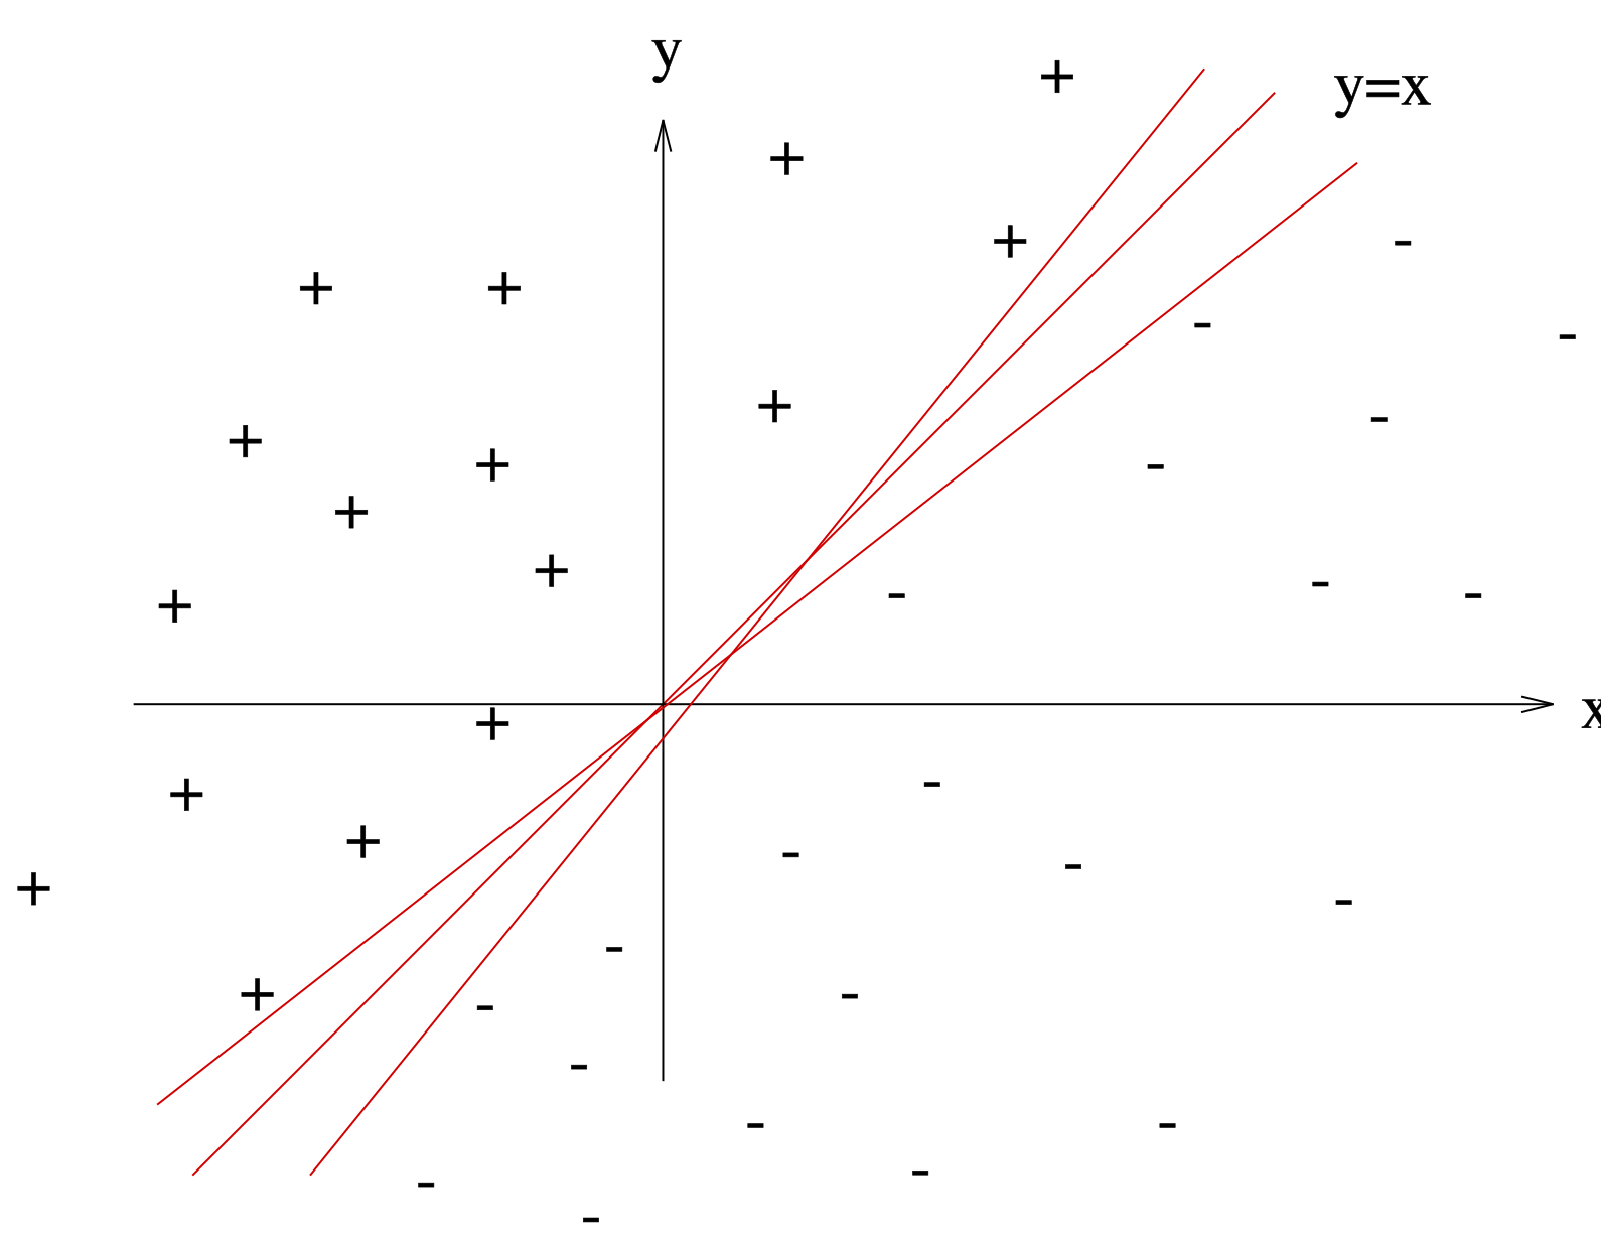
\includegraphics[width=\textwidth]{../images/pipeline/svm_multiple_boundaries.pdf}
        \captionsetup{width=\linewidth}
        \captionsetup{justification=centering}
        \caption{Multiple equally good linear decision boundaries for the train data. Free figure by Sylenius, CC BY-SA 3.0, via Wikimedia Commons.}
        \label{fig:processing_signals_svm_boundary_multiple}
    \end{subfigure}
    \hfill
    \begin{subfigure}{0.45\textwidth}
        \centering
        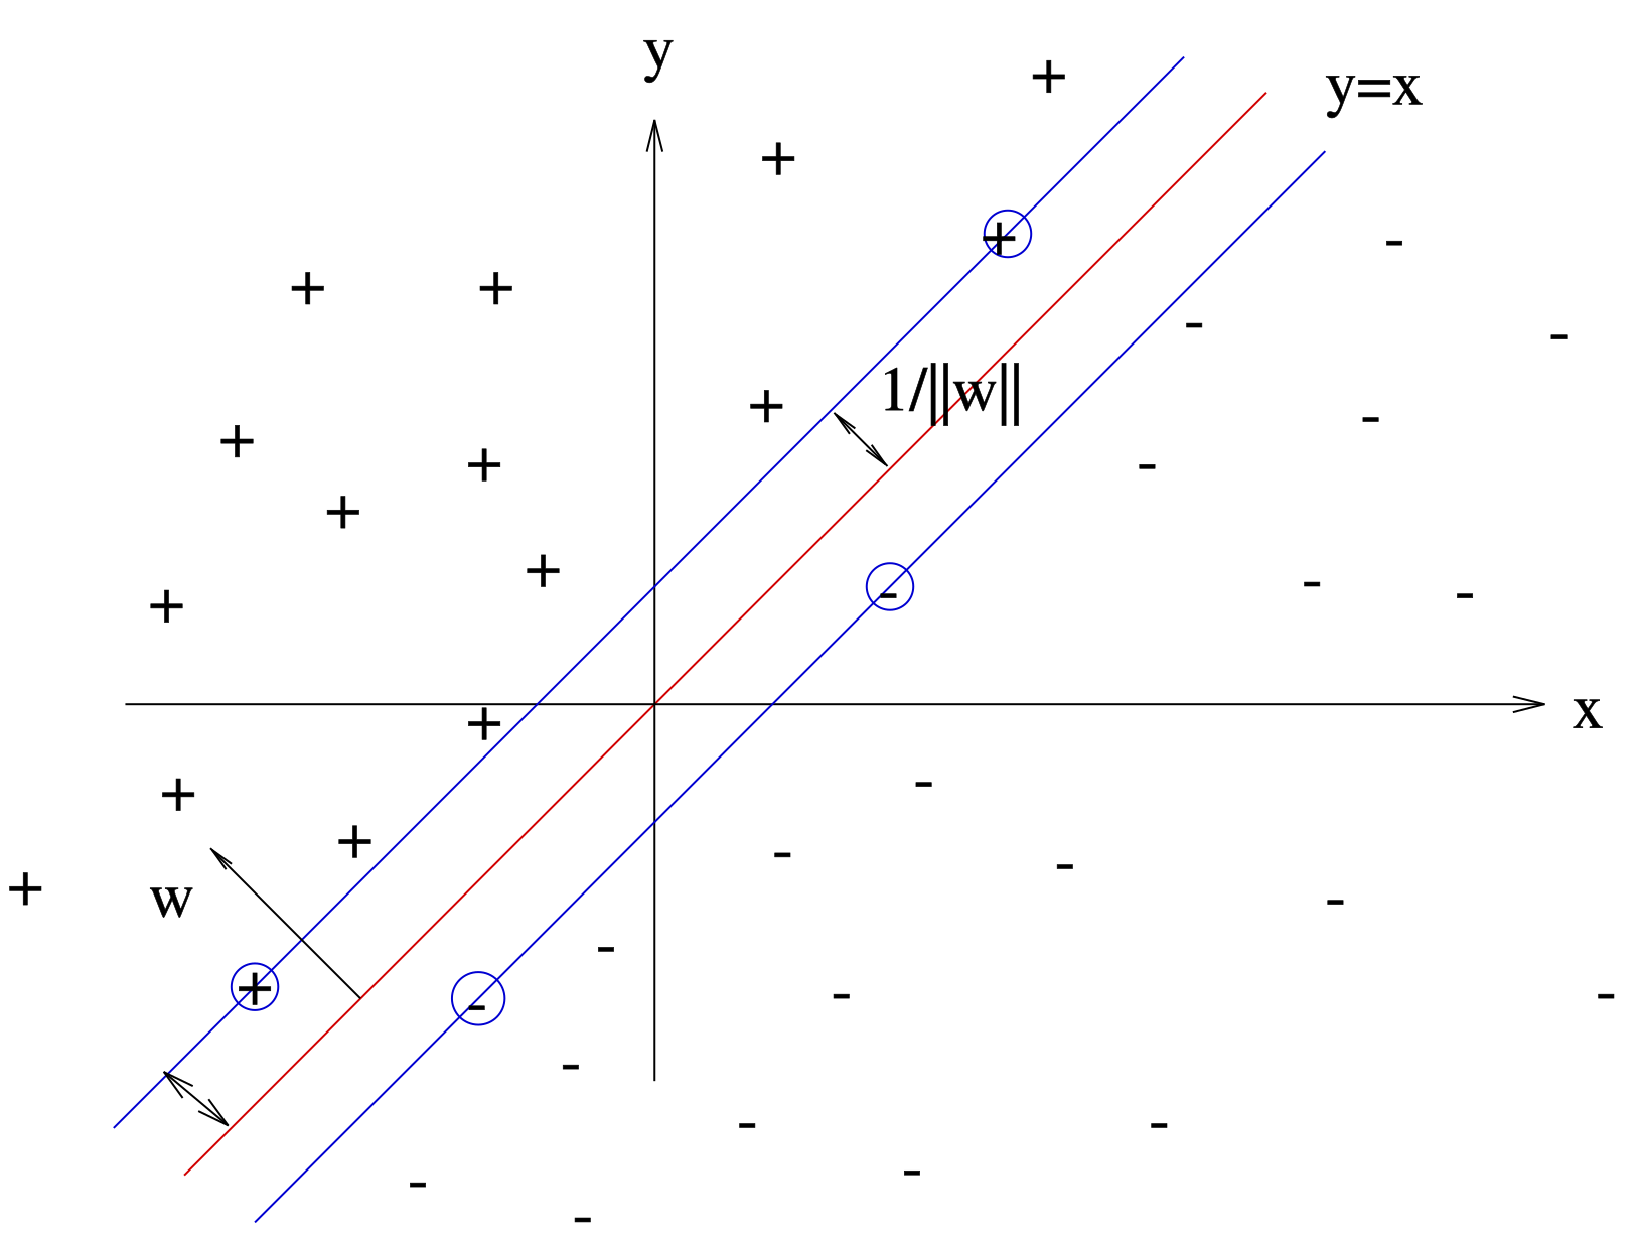
\includegraphics[width=\textwidth]{../images/pipeline/svm_best_boundary.pdf}
        \captionsetup{width=\linewidth}
        \captionsetup{justification=centering}
        \caption{The decision boundary chosen by SVM is based on the maximized distance to the support vectors. Free figure by Sylenius, CC BY-SA 3.0, via Wikimedia Commons.}
        \label{fig:processing_signals_svm_boundary_best}
    \end{subfigure}
    \captionsetup{width=\linewidth}
    \captionsetup{justification=centering}
    \caption{A linearly separable problem with multiple possibilities for decision boundaries.}
    \label{fig:processing_signals_svm_boundary}
\end{figure}


\Gls{svm} assumes that the best decision boundary is the one which maximizes the distance from the \textit{support vectors} to the decision boundary.
These support vectors are the points closest to the decision boundary.
Figure \ref{fig:processing_signals_svm_boundary_best} shows the decision boundary chosen by \gls{svm} based on the maximized distance from the support vectors circled in blue to the decision boundaries shown in red.
In higher dimensionality, this decision boundary becomes a hyperplane which can be described by Equation \ref{eq:processing_signals_svm_decission_boundary} where $\mathbf{W}$ is the weight vector normal to the hyperplane and $b$ is the bias.
The distance from a point $\mathbf{p}$ to this decision boundary can be calculated using Equation \ref{eq:processing_signals_svm_point_distance}.
$||\mathbf{w}||$ denotes the euclidean norm of the weight vector $\mathbf{W}$.

Since we assume a linear separation is possible, we know that for the training samples $\mathbf{x}_i$ with binary class label $y_i$ that Equation \ref{eq:processing_signals_svm_rules} holds.
Since scaling $y_i (\mathbf{w}^T \cdot \mathbf{x}_i + b)$ won't change the position of the hyperplane, it is possible to state that for a certain set $\mathbf{W}$ and $b$ the minimal value is 1 since the result will always be different from zero due to the linear separability assumption and the possibility of scaling.
As such, the distance to the hyperplane at the support vectors can be simplified from $\frac{y_i (\mathbf{w}^T \cdot \mathbf{x}_i + b)}{||\mathbf{w}||}$ to $\frac{1}{||\mathbf{w}||}$.
Maximizing $\frac{1}{||\mathbf{w}||}$ corresponds to minimzining $||\mathbf{w}||$ which is computationally easier and what is done by the \gls{svm} algorithm in an iterative way.


\begin{equation}
    \label{eq:processing_signals_svm_decission_boundary}
    \mathbf{w} \cdot \mathbf{x} + b = 0
\end{equation}

\begin{equation}
    \label{eq:processing_signals_svm_point_distance}
    \text{Distance to point } \mathbf{p} = \frac{\mathbf{w}^T \cdot \mathbf{p} + b}{||\mathbf{w}||}
\end{equation}

\begin{equation}
    \label{eq:processing_signals_svm_rules}
    \mathbf{w}^T \cdot \mathbf{x}_i + b 
    \begin{cases}
          < 0 & \text{if $y_i$ = -1} \\
          > 0 & \text{if $y_i$ = 1}
    \end{cases}
    \Longleftrightarrow y_i (\mathbf{w}^T \cdot \mathbf{x}_i + b) > 0
\end{equation}

With the decision boundary in place, making predictions is trivial.
However, the calculations shown all assume a perfectly linearly separable problem, which is often not the case with real-world data and especially not with \gls{eeg} data.
When making this assumption, the \gls{svm} approach is reffered to as \textit{hard margin} \gls{svm} classification.
To allow for classifying in non-linearly separable problems, \textit{soft margin} \gls{svm} classification has to be used.
Soft margin \gls{svm} classification assumes the samples that stop the linear separation from being possible are noise and can be ignored.
Mathematically this is done by changing the minimum condition from $y_i (\mathbf{w}^T \cdot \mathbf{x}_i + b) = 1$ to $y_i (\mathbf{w}^T \cdot \mathbf{x}_i + b) = 1 - \xi_i$.
$\xi_i$ is called the slack variable and \citet{svm_explained} explains in greater detail how it can be controlled by the hyperparameter $C$, which makes a tradeoff between the maximizing the margin and the number of misclassification on the training data.

Whilst the slack variable allows non-linearly separable problems to be learned by \gls{svm}, it assumes that the classification errors it makes are noise in the data.
As such, it only works well for data that is \textit{almost} linearly separable.
However, \gls{svm} has a clever mechanism for reducing non-linear problems to (almost) linear problems.
By finding a higher dimensional representation of the data, \gls{svm} can reduce a non-linear problem to a linear one.
This is known as the \textit{kernel trick} and an intuitive example is shown in Figure \ref{fig:processing_signals_svm_kernel}.
The specific transformation done in this figure is from 2D to 3D with the kernel function shown in Equation \ref{eq:processing_signals_svm_kernel_function}.
In practice, much more complex kernels are often used, with the most common ones being the linear kernel, the polynomial kernel and the \gls{rbf} kernel.
From these, the \gls{rbf} kernel is the most notable as its feature space has an infinite number of dimensions \citep{ml_book}.
Equation \ref{eq:processing_signals_svm_rbf} shows the \gls{rbf} kernel function.
By tuning the hyperparameter $\sigma$, the smoothness of the decision boundary in the original space can be controlled.

\begin{equation}
    \label{eq:processing_signals_svm_kernel_function}
    \Phi ((x_1, x_2)) = (x_1, x_2, x_1^2 + x_2^2)
\end{equation}

\begin{equation}
    \label{eq:processing_signals_svm_rbf}
    \Phi ((\mathbf{x}, \mathbf{x}')) = \exp(- \frac{|| \mathbf{x} - \mathbf{x}' ||^2}{2 \sigma^2} )
\end{equation}

\begin{figure}[t]
    \centering
    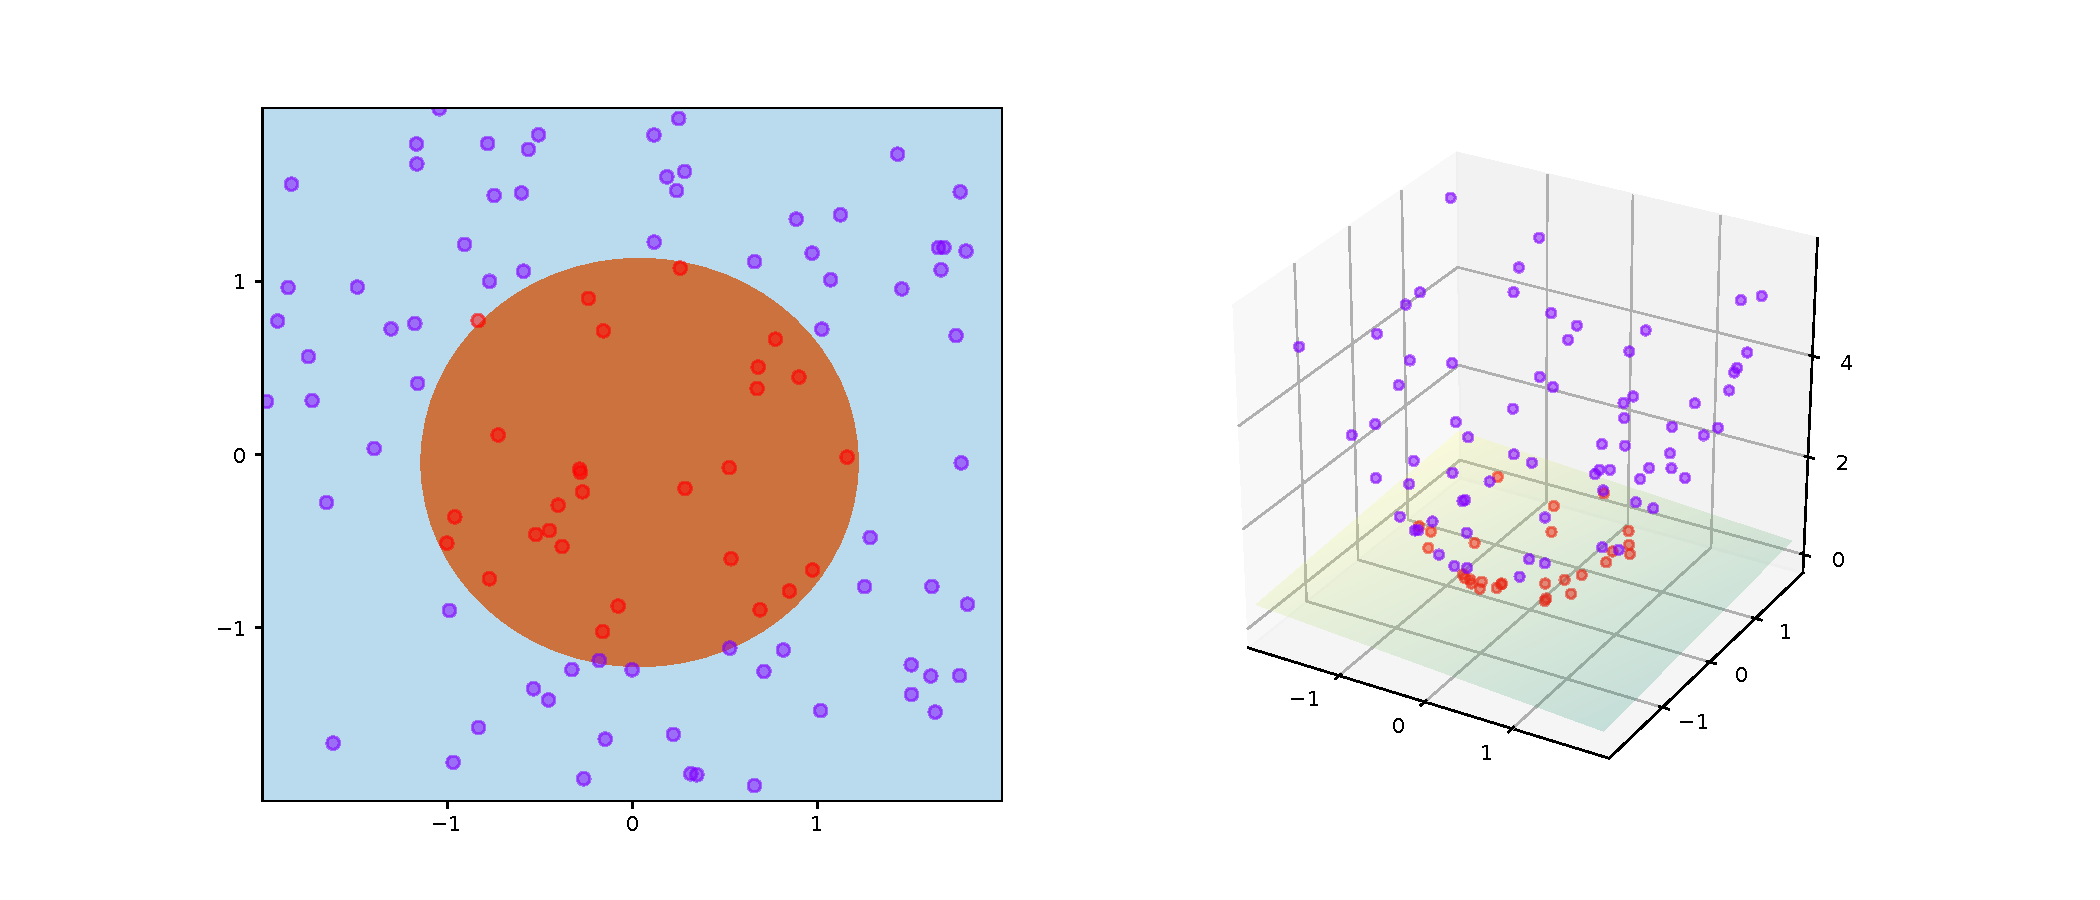
\includegraphics[width=\linewidth]{../images/pipeline/svm_kernel_trick.pdf}
    \captionsetup{width=0.8\linewidth}
    \captionsetup{justification=centering}
    \caption{An intuitive example of SVM's kernel trick where a 2D non-linearly separable problem is transformed into a 3D problem where it is linearly separable. Free to use Figure by Shiyu Ji, CC BY-SA 4.0, via Wikimedia Commons.}
    \label{fig:processing_signals_svm_kernel}
\end{figure}

% | | | | | | | | | | | | |

\subsubsection{Random forest (RF)}
\label{subsubsec:processing_signals_ml_and_dl_ml_classifiers_rf}

% TODO: start here, with LDA being simple SVM capable byt many hyperparameters and poor explainibility due to high dimension, we opt for RF which ...
% Besrpreken dat je kan visualiseren

TODO 


% - - - - - - - - - -
% Common DL classifiers
% - - - - - - - - - -

\subsection{Common one-step DL classifier layers}
\label{subsec:processing_signals_ml_and_dl_dl_classifiers}

% Shallow vs deep learning uitleggen
% Zie file:///Users/lennertbontinck/Library/CloudStorage/OneDrive-VrijeUniversiteitBrussel/SEM%202/Master%20thesis/books/ml_book.pdf

% ANN (MLP fully connected -> wanneer DL en wanneer regular ML, uitleggen soms gezienals regular ML)
% CNN (conv layer, pooling layer)
% RNN (e.g. long term short term memory voor die layer)
% Zie Alexis en wolf (classification)?

% These approaches have been chosen because of their relevance to this thesis. For a more detailed review of deep learning approaches for EEG classification, the reader is referred to the works of Roy et al. (2019) and Craik et al. (2019). wolf

% Veel al discussed in bci_opportunities_obstacles_motivating_examples_mi_models (BCIs)

% TODO: cnn bespreken a la: The most common type of DL neural networks at this time are the previously described CNNs (LeCun et al 1989). The subsequent application of convolutional layers results in a high-level representation of the input as stipulated by Goodfellow et al (2016). For example, in an object classification task, the network learns to extract primitive shapes from the raw input (a matrix of pixel values) in the first layer and then learns to extract objects from these primitive features in the next layer.
% en dus niet perse laatste layers voor classification maar vaak laatste layers terug mlps oid ipv puur convolutional layer

% In practice, neural networks can combine many layers of different kinds. It is not unusual to find neural networks that start with a few convolutional layers, to detect patterns independently of where they are in the input (such as edges in an image, or features in a 1D signal), then have one LSTM layer to be able to make sense of sequences of inputs, followed by a few feed-forward MLP-like layers to map what the LSTM layer learned to actual outputs. In the papers that we review in this article, great care is always given to explain and motivate the choice of neural architecture. Designing a neural network requires experience, as there is no systematic approach. We refer readers interested in knowing more than what we present here to books such as Goodfellow et al (2016) and Aggarwal (2018).


% The dominance of CNN with regard to model choice can be attributed to the relative ease of use and the popularity of this architecture in other research fields that use DL. While RNN architectures have been successful in closely related fields such as speech recognition and natural language processing, they have only seen limited deployment in a biosignal decoding context. Typically, CNNs also have less trainable parameters which makes them less sensitive to small datasets and lower their computational requirements. Other architectures were investigated for biosignal decoding, but state-of-the-art research mostly focuses on CNN architectures (Buongiorno et al 2019, Roy et al 2019).

% nog een pro CNN en waarom wij focussen op CNN: The choice of DL model is highly dependent on the application requirements and how the data is preprocessed. CNNs can often work with raw data that is only cleaned in the preprocessing step, while other models will typically necessitate feature extraction before passing the input to the ANN (Schirrmeister et al 2017). Alternatively, RNNs are also used for biosignal decoding, but these architectures typically need more technical knowledge to deploy and evaluate. The literature review clearly shows that CNN is the most deployed model and that biosignal decoding models are typically rather shallow, which can be attributed to the limited availability of data.


% Designing a neural network requires experience, as there is no systematic approach. More information on neural networks and their architectures is presented in the appendix, section ‘Neural networks’.



% bekijk ml_strats_used_in_papers

TODO
The most important concepts of \gls{dl} with respect to this master thesis will also be discussed, including fully connected layers (as seen in \glspl{ann}), convolutional layers and pooling layers (as seen in \glspl{cnn}) along with various important concepts such as dropout, batch normalization and activation functions.

% ---------------------------------------------- 
% EVALUATING AND USING
% ---------------------------------------------- 
\section{Using and evaluating the classification pipeline}
\label{sec:processing_signals_evaluating_and_using}

% link back naar pipeline van cad

% duidelijk bespreken welk ding echt CS en welk ding eigenlijk derden

TODO

% - - - - - - - - - -
% trianing vs prediction
% - - - - - - - - - -

\subsection{Difference between training and prediction pipeline}
\label{subsec:processing_signals_evaluating_and_using_training_vs_prediction}

TODO

% - - - - - - - - - -
% offline vs online
% - - - - - - - - - -

\subsection{Difference between offline and online prediction}
\label{subsec:processing_signals_evaluating_and_using_offline_vs_online}

TODO

% - - - - - - - - - -
% calibration
% - - - - - - - - - -

\subsection{Calibrating a previously trained pipeline}
\label{subsec:processing_signals_evaluating_and_using_calibration}

TODO

% - - - - - - - - - -
% evaluting
% - - - - - - - - - -

\subsection{Evaluating the performance of the pipeline}
\label{subsec:processing_signals_evaluating_and_using_evaluation}

% CM
% acc
% loss
% f1
% ppv npv etc?
% CV 

TODO


% - - - - - - - - - -
% evaluting
% - - - - - - - - - -

\subsection{Hyperparameter tuning}
\label{subsec:processing_signals_evaluating_and_using_hyperparameter_tuning}

TODO

% ---------------------------------------------- 
% COMMON ISSUES
% ---------------------------------------------- 

\section{Common issues with MI classification pipelines}
\label{sec:processing_signals_common_issues}

TODO

% - - - - - - - - - -
% biased data
% - - - - - - - - - -

\subsection{Biased data}
\label{subsec:processing_signals_common_issues_bias}

TODO

% - - - - - - - - - -
% evaluation
% - - - - - - - - - -

\subsection{Incorrect or ambiguous evaluation}
\label{subsec:processing_signals_common_issues_generalisation}
% e.g. only look at a person we also used in training etc

TODO

% - - - - - - - - - -
% explainability and interpretability
% - - - - - - - - - -

\subsection{No explainability or interpretability}
\label{subsec:processing_signals_common_issues_exaplainable}

TODO

% TOODO
\Gls{dl} often requires significant processing power and time to train, impacting the affordability of \gls{bci} research.
This is especially true when working with many \gls{eeg} sensors and features, and thus a high dimensional setting. 
\Gls{dl} is often also used in a black-box principle.
This means that the trained system lacks explainability and interpretability.
% TODO explain both terms
Recent governmental reports have suggested that laws will be coming in place to require these properties \citep{eu_ai_blackbox_report, explainable_ai_policy}.

% - - - - - - - - - -
% overfitting
% - - - - - - - - - -

\subsection{Overfitting}
\label{subsec:processing_signals_common_issues_overfitting}

% To avoid over-fitting, Batch Normalization (Ioffe and Szegedy 2015) considers the input of every layer in a neural network, and normalizes it so that, in expectation, the inputs of every layer has a zero mean and a unit variance. Dropout (Srivastava et al 2014) does not modify the values that flow through a neural network, but instead randomly disables neurons every time the network is evaluated during training. Both these methods contribute to improving training speed and generalization of the network, and ensure that the model converges to an optimal loss. Both batch normalization (Tayeb et al 2019, Tam et al 2020) and dropout (Gautam et al 2020, Tortora et al 2020a) are often used in biosignal decoding papers, sometimes both at the same time. Other normalization techniques are possible, such as L1- normalization or clipping the gradients (Zhang et al 2019a), but they have been superseded by Batch Normalization and Dropout.

% generalization bespreken: With neural networks, the main avenue to increase generalization is to decrease over-fitting. Over-fitting happens when a neural network remembers exactly what training input should learn which training output, without having actually made sense of the data. The network achieves a training loss close to 0, but produces garbage output on the testing set. It is like a small child that learns how to read words, and remembers that card number 7 is pronounced ‘cat’, without actually looking at the word written on the card, or being able to read at all. Batch normalization (Ioffe and Szegedy 2015) considers the input of every layer in a neural network, and normalizes it so that, in expectation, the inputs of every layer has a zero mean and a unit variance. Intuitively, this normalization prevents ludicrously large or small values from appearing inside the network, which makes it ‘behave better’ or ‘be smoother’ (so, easier to train, and better at generalization). The actual mathematical way in which batch normalization works is however still unknown, with recent papers providing the first insights (Santurkar et al 2018). Dropout (Srivastava et al 2014) does not modify the values that flow through a neural network, but instead randomly disables neurons every time the network is evaluated during training. The main motivation behind Dropout is to avoid one particular neuron in the network to learn how to compensate (and thus cancel out) another particular neuron in the network. When neurons are constantly randomly disabled and re-enabled, they all have to learn independently from each other. More mathematically, Dropout leads to a neural network that is made of a different set of neurons every time it is evaluated. This leads to a large ensemble of ‘sub-networks’, all trained on different datapoints. Ensembles of function approximators such as this are known to help with generalization (Dietterich 2000). Both batch normalization (Tayeb et al 2019, Tam et al 2020) and Dropout (Gautam et al 2020, Tortora et al 2020a) are often used in biosignal decoding papers, sometimes both at the same time. Other normalization techniques are possible, such as L1- normalization or clipping the gradients (Zhang et al 2019a), but they have been superseded by Batch Normalization and Dropout.

% uit bci_review_arnau

TODO

% ---------------------------------------------- 
% CONCLUSIONS OF CHAPTER
% ---------------------------------------------- 
\section{Motivation for offline classification and chapter conclusions}
\label{sec:processing_signals_summary}
% TODO: summary of this chapter

% duidelijk bespreken classificiation echt CS terwijl die contorl vaak een andere (buiten interface ofc) ook link naar die paper division door ons
% bespreken paper division door ons zegt dat on classi model bruikbaar moet zijn maar dit nog net iets anders want offline, dus is eigenlijk nog further subdivision

TODO
% TODO:
%   - XXX
% ----------  
% Questions:
%   - XXX

% TODO: gans herschrijven want is nu eig 6_xxx en dan hier echt een implementatie doen
% dit gaat met veel refs messen dus zeker nazien

% Uncomment this if the use of parts is desired
\part{Implementing an EEG-based brain-computer interface that classifies motor imagery tasks}

% iets a la hiervoor gezien hoe besproken en nu effectief hoe doen

% Checkout Fieldtrip toolbox voor laplacian

\chapter{EEG-based offline classification system for motor imagery tasks}
\label{ch:offline_bci_system}
TODO

\section{Training the system}
\label{sec:bci_pipeline_training}
TODO


\subsection{Data gathering and windowing}
\label{subsec:bci_pipeline_training_data_gathering_windowing}

% Several windowing methods exist and are reviewed by Podder et al (2014).

% Windowing: when specific events in a signal (such as a spike or pattern) matters more than the overall shape of the complete signal, windowing allows to split a signal into fixed-length, usually overlapping, sub-sequences. Having the network focus on small sub-sequences allows it to be faster (less compute intensive, as less data is being processed), and generalize better, as a small number of easily-recognizable patterns (on which the network focuses) can appear in various positions in longer signals (that the network does not have to bother with). Several windowing methods exist, and are reviewed by Podder et al (2014). Jeong et al (2020) and Nguyen and Chung (2019) use Hamming windowing.

TODO


\subsection{Pre-processing}
\label{subsec:bci_pipeline_training_preprocessing}

% as discussed by review arnau: Limit required preprocessing: extensive preprocessing will yield clean signals with a high SNR, but this usually comes at the cost of expensive computational requirements that take resources and time. It will often be necessary to balance preprocessing requirements with latency and power consumption constraints.

% Conceptually, given enough layers and neurons, and the proper architecture, a neural network can learn any mapping from inputs to outputs (Sonoda and Murata 2017) (they are universal function approximators). This means that any method of acquiring a signal, and representing it as floatingpoint values will eventually allow the network to make sense of the inputs, and learn something. However, a more careful design of the inputs allows to improve two important properties of the neural network: learning speed (important when the network is used in an adaptive system that learns as it is being used) and generalization power (the ability of making high-quality predictions for unseen inputs, even if training on a small amount of input-output pairs). Designing the input, also called feature engineering, is highly domain-specific. In the signal processing literature, especially in settings that consider EEG data

% Signal filtering: applied on the signals, filters remove frequencies of the signals, to only keep those of interest. This is a form of noise removal, in which the expert designer knows that some frequencies never convey information and can only be noise. There are many different types of filters, which fall outside of the scope of this publication. For more information on filters and digital signal processing, interested readers are referred to (Orfanidis 1996).

TODO


\subsection{Feature extraction and generation}
\label{subsec:bci_pipeline_training_features}
TODO

% Feature extraction: this final step is highly variable and depends on the exact context (sleep staging, Motor Imagery detection, epilepsy seizure detection, etc) in which the signal should be decoded. In general, DL models have been shown to perform better when the input is the raw (preprocessed) signal that is still represented as timeseries of samples for each signal channel. One of the most commonly used feature extraction methods is the Fourier transform, which allows to decompose a temporal signal (a sequence of signal readings over time) to a sum of sinuses of various frequencies. The Fourier transform transforms data from the time domain to the frequency domain. This transform is loss-less and invertible, which means that it does not destroy information. It allows the neural network to more easily focus on the existence of a particular frequency in a signal, instead of having to make sense of the entire (time-domain) signal.

% For a detailed review of possible feature extraction methods, we refer interested readers to Rashid et al (2020).


\subsection{Training a ML classification model}
\label{subsec:bci_pipeline_training_classification_model}
TODO

\section{Using the system}
\label{sec:bci_pipeline_using}
TODO


\subsection{Applying the trained classifier}
\label{subsec:bci_pipeline_using_classifier}
TODO


\subsection{Moving towards an online system}
\label{subsec:bci_pipeline_using_going_online}
TODO


% TODO:
%   - XXX
% ----------  
% Questions:
%   - XXX

% zeggen dat voor bepalen van uw systeem dat ge wilt doen moet ge zien naar arnau zijn review: 5.2. A literature-based guide to DL for biosignal control

% Efforts are being made to develop standardized platforms that facilitate the deployment of control systems into real or simulated environments. Previous research solutions attempted to create common ecosystems for neurorobotic applications, in terms of open source frameworks such as the Neurorobotics platform (Falotico et al 2017), ROS-Health (Beraldo et al 2018) and its successor ROS-Neuro (Tonin et al 2019). ROS-Neuro was already succesfully used in a DL context (Valenti et al 2020, 2021). For more general applications, the OpenVibe platform provides several environments and integrates with a large variety of devices for BCI control experiments (Renard et al 2010).

% feedback is belangrijk en kan soms voor actie zijn om dan te cancellen met bv eye movement oid

\chapter{Moving from an offline classification system towards an online BCI system}
\label{ch:online_bci_system}
TODO

% TODO:
%   - XXX
% ----------  
% Questions:
%   - XXX

% technology readiness level bespreken?

% Cohen's kappa value

% Uncomment this if the use of parts is desired
\part{Reflection on the results of this thesis}

\chapter{Using the system and verifying the results}
\label{ch:evaluation}
TODO

% TODO:
%   - XXX
% ----------  
% Questions:
%   - XXX



% whilst user validation is neceasrry for final product, as poc according to arnau: Perform user studies: a user study is the only way to really evaluate the user experience of a control system. While validation is sufficient for an initial prototype, evaluation in the lab will be necessary at a higher technology readiness level. Finally, in-field evaluation is necessary to assess user experience in real-world operating conditions.

\chapter{Self-reflection and conclusions}
\label{ch:discussion}
TODO

% ---------------------------------------------- 
% INTRODUCTION
% ---------------------------------------------- 
\section{Introduction to this chapter}
\label{sec:discussion_introduction}
% NOTE: "Introduction" exists in each chapter and gives a short intro to the chapter + what can be expected in the chapter

TODO

% ---------------------------------------------- 
% usability
% ---------------------------------------------- 
\section{Real world usability of the obtained results}
\label{sec:discussion_real_world_use}

TODO

% ---------------------------------------------- 
% Added value
% ---------------------------------------------- 
\section{Added value of this master thesis}
\label{sec:discussion_added_value}

TODO

% ---------------------------------------------- 
% Future work
% ---------------------------------------------- 
\section{Future work}
\label{sec:discussion_future_work}

TODO

% ---------------------------------------------- 
% Conclusions
% ---------------------------------------------- 
\section{Final remarks and a personal endnote}
\label{sec:discussion_final_remarks}

TODO



\backmatter%

% Glossary
\glsaddall
\printnoidxglossary[type=\acronymtype,title=List of abbreviations, nonumberlist, style=listgroup]
%\addcontentsline{toc}{chapter}{List of abbreviations}

% References list (show even non cited)
\nocite{*}
\printbibliography[heading=bibintoc, title={References}]
\end{document}













